\documentclass[a4paper]{book}
\usepackage{makeidx}
\usepackage{natbib}
\usepackage{graphicx}
\usepackage{multicol}
\usepackage{float}
\usepackage{listings}
\usepackage{color}
\usepackage{ifthen}
\usepackage[table]{xcolor}
\usepackage{textcomp}
\usepackage{alltt}
\usepackage{ifpdf}
\ifpdf
\usepackage[pdftex,
            pagebackref=true,
            colorlinks=true,
            linkcolor=blue,
            unicode
           ]{hyperref}
\else
\usepackage[ps2pdf,
            pagebackref=true,
            colorlinks=true,
            linkcolor=blue,
            unicode
           ]{hyperref}
\usepackage{pspicture}
\fi
\usepackage[utf8]{inputenc}
\usepackage{mathptmx}
\usepackage[scaled=.90]{helvet}
\usepackage{courier}
\usepackage{sectsty}
\usepackage[titles]{tocloft}
\usepackage{doxygen}
\lstset{language=C++,inputencoding=utf8,basicstyle=\footnotesize,breaklines=true,breakatwhitespace=true,tabsize=8,numbers=left }
\makeindex
\setcounter{tocdepth}{3}
\renewcommand{\footrulewidth}{0.4pt}
\renewcommand{\familydefault}{\sfdefault}
\hfuzz=15pt
\setlength{\emergencystretch}{15pt}
\hbadness=750
\tolerance=750
\begin{document}
\hypersetup{pageanchor=false,citecolor=blue}
\begin{titlepage}
\vspace*{7cm}
\begin{center}
{\Large \-S\-T\-A\-R\-K \-V\-M\-S }\\
\vspace*{1cm}
{\large \-Generated by Doxygen 1.7.6.1}\\
\vspace*{0.5cm}
{\small Wed Dec 11 2013 10:44:49}\\
\end{center}
\end{titlepage}
\clearemptydoublepage
\pagenumbering{roman}
\tableofcontents
\clearemptydoublepage
\pagenumbering{arabic}
\hypersetup{pageanchor=true,citecolor=blue}
\chapter{\-Namespace \-Index}
\section{\-Namespace \-List}
\-Here is a list of all namespaces with brief descriptions\-:\begin{DoxyCompactList}
\item\contentsline{section}{\hyperlink{namespaceGrammar}{\-Grammar} }{\pageref{d0/da6/namespaceGrammar}}{}
\item\contentsline{section}{\hyperlink{namespaceparser}{parser} }{\pageref{d0/dd5/namespaceparser}}{}
\item\contentsline{section}{\hyperlink{namespacePDA}{\-P\-D\-A} }{\pageref{d7/d11/namespacePDA}}{}
\item\contentsline{section}{\hyperlink{namespaceTM}{\-T\-M} }{\pageref{d6/d65/namespaceTM}}{}
\item\contentsline{section}{\hyperlink{namespaceutilities}{utilities} }{\pageref{d2/d96/namespaceutilities}}{}
\end{DoxyCompactList}

\chapter{\-Class \-Index}
\section{Class Hierarchy}
This inheritance list is sorted roughly, but not completely, alphabetically\-:\begin{DoxyCompactList}
\item \contentsline{section}{C\-F\-G}{\pageref{d7/dd4/classCFG}}{}
\begin{DoxyCompactList}
\item \contentsline{section}{C\-N\-F\-\_\-\-C\-F\-G}{\pageref{da/d5c/classCNF__CFG}}{}
\end{DoxyCompactList}
\item \contentsline{section}{C\-Y\-K\-Table}{\pageref{d6/dcd/classCYKTable}}{}
\item exception\begin{DoxyCompactList}
\item \contentsline{section}{Exception}{\pageref{d4/d67/classException}}{}
\end{DoxyCompactList}
\item \contentsline{section}{Parser}{\pageref{d0/d40/classParser}}{}
\begin{DoxyCompactList}
\item \contentsline{section}{C\-F\-G\-Parser}{\pageref{da/d24/classCFGParser}}{}
\item \contentsline{section}{L\-R\-Parser}{\pageref{d6/de9/classLRParser}}{}
\end{DoxyCompactList}
\item \contentsline{section}{Parse\-Table}{\pageref{d9/da1/classParseTable}}{}
\item \contentsline{section}{P\-D\-A\-:\-:P\-D\-A}{\pageref{d1/dc5/classPDA_1_1PDA}}{}
\item \contentsline{section}{P\-D\-A\-:\-:State}{\pageref{d7/d1f/classPDA_1_1State}}{}
\end{DoxyCompactList}

\chapter{\-Class \-Index}
\section{\-Class \-List}
\-Here are the classes, structs, unions and interfaces with brief descriptions\-:\begin{DoxyCompactList}
\item\contentsline{section}{\hyperlink{classCFG}{\-C\-F\-G} }{\pageref{d7/dd4/classCFG}}{}
\item\contentsline{section}{\hyperlink{classCFGParser}{\-C\-F\-G\-Parser} }{\pageref{da/d24/classCFGParser}}{}
\item\contentsline{section}{\hyperlink{classCNF__CFG}{\-C\-N\-F\-\_\-\-C\-F\-G} }{\pageref{da/d5c/classCNF__CFG}}{}
\item\contentsline{section}{\hyperlink{classCYKTable}{\-C\-Y\-K\-Table} }{\pageref{d6/dcd/classCYKTable}}{}
\item\contentsline{section}{\hyperlink{classException}{\-Exception} }{\pageref{d4/d67/classException}}{}
\item\contentsline{section}{\hyperlink{classLRParser}{\-L\-R\-Parser} }{\pageref{d6/de9/classLRParser}}{}
\item\contentsline{section}{\hyperlink{classParser}{\-Parser} }{\pageref{d0/d40/classParser}}{}
\item\contentsline{section}{\hyperlink{classParseTable}{\-Parse\-Table} }{\pageref{d9/da1/classParseTable}}{}
\item\contentsline{section}{\hyperlink{classPDA_1_1PDA}{\-P\-D\-A\-::\-P\-D\-A} }{\pageref{d1/dc5/classPDA_1_1PDA}}{}
\item\contentsline{section}{\hyperlink{classPDA_1_1State}{\-P\-D\-A\-::\-State} }{\pageref{d7/d1f/classPDA_1_1State}}{}
\end{DoxyCompactList}

\chapter{\-File \-Index}
\section{\-File \-List}
\-Here is a list of all files with brief descriptions\-:\begin{DoxyCompactList}
\item\contentsline{section}{src/\hyperlink{CFG_8h}{\-C\-F\-G.\-h} }{\pageref{d9/d25/CFG_8h}}{}
\item\contentsline{section}{src/\hyperlink{CYKTable_8h}{\-C\-Y\-K\-Table.\-h} }{\pageref{db/d5c/CYKTable_8h}}{}
\item\contentsline{section}{src/\hyperlink{DesignByContract_8h}{\-Design\-By\-Contract.\-h} }{\pageref{d0/d30/DesignByContract_8h}}{}
\item\contentsline{section}{src/\hyperlink{Exception_8h}{\-Exception.\-h} }{\pageref{d8/d8a/Exception_8h}}{}
\item\contentsline{section}{src/\hyperlink{Information_8h}{\-Information.\-h} }{\pageref{d6/d92/Information_8h}}{}
\item\contentsline{section}{src/\hyperlink{LRParser_8h}{\-L\-R\-Parser.\-h} }{\pageref{de/db3/LRParser_8h}}{}
\item\contentsline{section}{src/\hyperlink{Parser_8h}{\-Parser.\-h} }{\pageref{d6/d0c/Parser_8h}}{}
\item\contentsline{section}{src/\hyperlink{ParseTable_8h}{\-Parse\-Table.\-h} }{\pageref{d4/d97/ParseTable_8h}}{}
\item\contentsline{section}{src/\hyperlink{PDA_8h}{\-P\-D\-A.\-h} }{\pageref{d5/d4a/PDA_8h}}{}
\item\contentsline{section}{src/\hyperlink{State_8h}{\-State.\-h} }{\pageref{dd/d99/State_8h}}{}
\item\contentsline{section}{src/\hyperlink{TMParser_8h}{\-T\-M\-Parser.\-h} }{\pageref{d9/d25/TMParser_8h}}{}
\item\contentsline{section}{src/\hyperlink{TuringMachine_8h}{\-Turing\-Machine.\-h} }{\pageref{d1/d44/TuringMachine_8h}}{}
\item\contentsline{section}{src/\hyperlink{utilities_8h}{utilities.\-h} }{\pageref{de/df0/utilities_8h}}{}
\end{DoxyCompactList}

\chapter{\-Namespace \-Documentation}
\hypertarget{namespaceGrammar}{\section{\-Grammar \-Namespace \-Reference}
\label{d0/da6/namespaceGrammar}\index{\-Grammar@{\-Grammar}}
}
\subsection*{\-Classes}
\begin{DoxyCompactItemize}
\item 
class \hyperlink{classGrammar_1_1CFG}{\-C\-F\-G}
\item 
class \hyperlink{classGrammar_1_1CNF__CFG}{\-C\-N\-F\-\_\-\-C\-F\-G}
\item 
class \hyperlink{classGrammar_1_1CYKTable}{\-C\-Y\-K\-Table}
\end{DoxyCompactItemize}

\hypertarget{namespaceparser}{\section{parser \-Namespace \-Reference}
\label{d0/dd5/namespaceparser}\index{parser@{parser}}
}
\subsection*{\-Classes}
\begin{DoxyCompactItemize}
\item 
class \hyperlink{classparser_1_1LRParser}{\-L\-R\-Parser}
\item 
class \hyperlink{classparser_1_1Parser}{\-Parser}
\item 
class \hyperlink{classparser_1_1CFGParser}{\-C\-F\-G\-Parser}
\item 
class \hyperlink{classparser_1_1ParseTable}{\-Parse\-Table}
\end{DoxyCompactItemize}
\subsection*{\-Enumerations}
\begin{DoxyCompactItemize}
\item 
enum \hyperlink{namespaceparser_a7a838229f5b5b20f185dfad9d362dbed}{\-E\-Action} \{ \*
\hyperlink{namespaceparser_a7a838229f5b5b20f185dfad9d362dbedaa0b431997906e4d0c453d7ba0fe1c744}{shift}, 
\hyperlink{namespaceparser_a7a838229f5b5b20f185dfad9d362dbeda175b62b0686c65910f72c0c4b7ff2c86}{reduction}, 
\hyperlink{namespaceparser_a7a838229f5b5b20f185dfad9d362dbedab009f2af27ebdb5b6829ee1614826576}{accept}, 
\hyperlink{namespaceparser_a7a838229f5b5b20f185dfad9d362dbedacce7c4f977d7145f234fd8f2691dab61}{jump}, 
\*
\hyperlink{namespaceparser_a7a838229f5b5b20f185dfad9d362dbeda0c4197e3086acf7d33bcf1a943d4754c}{blank}, 
\hyperlink{namespaceparser_a7a838229f5b5b20f185dfad9d362dbedaa02231033cc9e46e39eff451b2aeafb9}{error}
 \}
\end{DoxyCompactItemize}


\subsection{\-Enumeration \-Type \-Documentation}
\hypertarget{namespaceparser_a7a838229f5b5b20f185dfad9d362dbed}{\index{parser@{parser}!\-E\-Action@{\-E\-Action}}
\index{\-E\-Action@{\-E\-Action}!parser@{parser}}
\subsubsection[{\-E\-Action}]{\setlength{\rightskip}{0pt plus 5cm}enum {\bf parser\-::\-E\-Action}}}\label{d0/dd5/namespaceparser_a7a838229f5b5b20f185dfad9d362dbed}
\begin{Desc}
\item[\-Enumerator\-: ]\par
\begin{description}
\index{shift@{shift}!parser@{parser}}\index{parser@{parser}!shift@{shift}}\item[{\em 
\hypertarget{namespaceparser_a7a838229f5b5b20f185dfad9d362dbedaa0b431997906e4d0c453d7ba0fe1c744}{shift}\label{d0/dd5/namespaceparser_a7a838229f5b5b20f185dfad9d362dbedaa0b431997906e4d0c453d7ba0fe1c744}
}]\index{reduction@{reduction}!parser@{parser}}\index{parser@{parser}!reduction@{reduction}}\item[{\em 
\hypertarget{namespaceparser_a7a838229f5b5b20f185dfad9d362dbeda175b62b0686c65910f72c0c4b7ff2c86}{reduction}\label{d0/dd5/namespaceparser_a7a838229f5b5b20f185dfad9d362dbeda175b62b0686c65910f72c0c4b7ff2c86}
}]\index{accept@{accept}!parser@{parser}}\index{parser@{parser}!accept@{accept}}\item[{\em 
\hypertarget{namespaceparser_a7a838229f5b5b20f185dfad9d362dbedab009f2af27ebdb5b6829ee1614826576}{accept}\label{d0/dd5/namespaceparser_a7a838229f5b5b20f185dfad9d362dbedab009f2af27ebdb5b6829ee1614826576}
}]\index{jump@{jump}!parser@{parser}}\index{parser@{parser}!jump@{jump}}\item[{\em 
\hypertarget{namespaceparser_a7a838229f5b5b20f185dfad9d362dbedacce7c4f977d7145f234fd8f2691dab61}{jump}\label{d0/dd5/namespaceparser_a7a838229f5b5b20f185dfad9d362dbedacce7c4f977d7145f234fd8f2691dab61}
}]\index{blank@{blank}!parser@{parser}}\index{parser@{parser}!blank@{blank}}\item[{\em 
\hypertarget{namespaceparser_a7a838229f5b5b20f185dfad9d362dbeda0c4197e3086acf7d33bcf1a943d4754c}{blank}\label{d0/dd5/namespaceparser_a7a838229f5b5b20f185dfad9d362dbeda0c4197e3086acf7d33bcf1a943d4754c}
}]\index{error@{error}!parser@{parser}}\index{parser@{parser}!error@{error}}\item[{\em 
\hypertarget{namespaceparser_a7a838229f5b5b20f185dfad9d362dbedaa02231033cc9e46e39eff451b2aeafb9}{error}\label{d0/dd5/namespaceparser_a7a838229f5b5b20f185dfad9d362dbedaa02231033cc9e46e39eff451b2aeafb9}
}]\end{description}
\end{Desc}


\hypertarget{namespacePDA}{\section{\-P\-D\-A \-Namespace \-Reference}
\label{d7/d11/namespacePDA}\index{\-P\-D\-A@{\-P\-D\-A}}
}
\subsection*{\-Classes}
\begin{DoxyCompactItemize}
\item 
class \hyperlink{classPDA_1_1PDA}{\-P\-D\-A}
\item 
class \hyperlink{classPDA_1_1State}{\-State}
\end{DoxyCompactItemize}
\subsection*{\-Enumerations}
\begin{DoxyCompactItemize}
\item 
enum \hyperlink{namespacePDA_a2f2b17cdf30facf6f0fe593ab209acf8}{\-P\-D\-A\-Type} \{ \hyperlink{namespacePDA_a2f2b17cdf30facf6f0fe593ab209acf8abec96ee068d9af07a9bf41137e3b3635}{accept\-By\-Empty\-Stack}, 
\hyperlink{namespacePDA_a2f2b17cdf30facf6f0fe593ab209acf8a68e7e330c1fb2405ce07c4f2600139e1}{accept\-By\-Final\-State}
 \}
\end{DoxyCompactItemize}


\subsection{\-Enumeration \-Type \-Documentation}
\hypertarget{namespacePDA_a2f2b17cdf30facf6f0fe593ab209acf8}{\index{\-P\-D\-A@{\-P\-D\-A}!\-P\-D\-A\-Type@{\-P\-D\-A\-Type}}
\index{\-P\-D\-A\-Type@{\-P\-D\-A\-Type}!PDA@{\-P\-D\-A}}
\subsubsection[{\-P\-D\-A\-Type}]{\setlength{\rightskip}{0pt plus 5cm}enum {\bf \-P\-D\-A\-::\-P\-D\-A\-Type}}}\label{d7/d11/namespacePDA_a2f2b17cdf30facf6f0fe593ab209acf8}
\begin{Desc}
\item[\-Enumerator\-: ]\par
\begin{description}
\index{accept\-By\-Empty\-Stack@{accept\-By\-Empty\-Stack}!\-P\-D\-A@{\-P\-D\-A}}\index{\-P\-D\-A@{\-P\-D\-A}!accept\-By\-Empty\-Stack@{accept\-By\-Empty\-Stack}}\item[{\em 
\hypertarget{namespacePDA_a2f2b17cdf30facf6f0fe593ab209acf8abec96ee068d9af07a9bf41137e3b3635}{accept\-By\-Empty\-Stack}\label{d7/d11/namespacePDA_a2f2b17cdf30facf6f0fe593ab209acf8abec96ee068d9af07a9bf41137e3b3635}
}]\index{accept\-By\-Final\-State@{accept\-By\-Final\-State}!\-P\-D\-A@{\-P\-D\-A}}\index{\-P\-D\-A@{\-P\-D\-A}!accept\-By\-Final\-State@{accept\-By\-Final\-State}}\item[{\em 
\hypertarget{namespacePDA_a2f2b17cdf30facf6f0fe593ab209acf8a68e7e330c1fb2405ce07c4f2600139e1}{accept\-By\-Final\-State}\label{d7/d11/namespacePDA_a2f2b17cdf30facf6f0fe593ab209acf8a68e7e330c1fb2405ce07c4f2600139e1}
}]\end{description}
\end{Desc}


\hypertarget{namespaceTM}{\section{\-T\-M \-Namespace \-Reference}
\label{d6/d65/namespaceTM}\index{\-T\-M@{\-T\-M}}
}
\subsection*{\-Classes}
\begin{DoxyCompactItemize}
\item 
class \hyperlink{classTM_1_1TuringMachine}{\-Turing\-Machine}
\end{DoxyCompactItemize}
\subsection*{\-Typedefs}
\begin{DoxyCompactItemize}
\item 
typedef std\-::string \hyperlink{namespaceTM_a852554502c474841ede5736b807839ff}{\-State\-Name}
\item 
typedef unsigned char \hyperlink{namespaceTM_af53c0529f78dfcdeb19c450abbd44cf6}{\-Tape\-Symbol}
\item 
typedef std\-::vector$<$ \hyperlink{namespaceTM_af53c0529f78dfcdeb19c450abbd44cf6}{\-Tape\-Symbol} $>$ \hyperlink{namespaceTM_a20b31cfe7d86b00db299e72ad48f70af}{\-Tape}
\item 
typedef std\-::tuple$<$ \hyperlink{namespaceTM_a852554502c474841ede5736b807839ff}{\-State\-Name}, \*
\hyperlink{namespaceTM_af53c0529f78dfcdeb19c450abbd44cf6}{\-Tape\-Symbol}, \hyperlink{namespaceTM_af53c0529f78dfcdeb19c450abbd44cf6}{\-Tape\-Symbol}, \*
\hyperlink{namespaceTM_a7c40dddb5b66504639e0d378ec13792d}{\-Direction}, \hyperlink{namespaceTM_a852554502c474841ede5736b807839ff}{\-State\-Name} $>$ \hyperlink{namespaceTM_a87460339f40338ea4e37433443965554}{\-Production}
\end{DoxyCompactItemize}
\subsection*{\-Enumerations}
\begin{DoxyCompactItemize}
\item 
enum \hyperlink{namespaceTM_a7c40dddb5b66504639e0d378ec13792d}{\-Direction} \{ \hyperlink{namespaceTM_a7c40dddb5b66504639e0d378ec13792dac3682a7842c29b64f35ecbeb70fafb7f}{left} =  0, 
\hyperlink{namespaceTM_a7c40dddb5b66504639e0d378ec13792da7524c80fbbe2893a839a75c97def5911}{right}, 
\hyperlink{namespaceTM_a7c40dddb5b66504639e0d378ec13792dabf7f6892ad2d17d8e27921834d7c3ee2}{none}
 \}
\end{DoxyCompactItemize}


\subsection{\-Typedef \-Documentation}
\hypertarget{namespaceTM_a87460339f40338ea4e37433443965554}{\index{\-T\-M@{\-T\-M}!\-Production@{\-Production}}
\index{\-Production@{\-Production}!TM@{\-T\-M}}
\subsubsection[{\-Production}]{\setlength{\rightskip}{0pt plus 5cm}typedef std\-::tuple$<${\bf \-State\-Name}, {\bf \-Tape\-Symbol}, {\bf \-Tape\-Symbol}, {\bf \-Direction}, {\bf \-State\-Name}$>$ {\bf \-T\-M\-::\-Production}}}\label{d6/d65/namespaceTM_a87460339f40338ea4e37433443965554}
\hypertarget{namespaceTM_a852554502c474841ede5736b807839ff}{\index{\-T\-M@{\-T\-M}!\-State\-Name@{\-State\-Name}}
\index{\-State\-Name@{\-State\-Name}!TM@{\-T\-M}}
\subsubsection[{\-State\-Name}]{\setlength{\rightskip}{0pt plus 5cm}typedef std\-::string {\bf \-T\-M\-::\-State\-Name}}}\label{d6/d65/namespaceTM_a852554502c474841ede5736b807839ff}
\hypertarget{namespaceTM_a20b31cfe7d86b00db299e72ad48f70af}{\index{\-T\-M@{\-T\-M}!\-Tape@{\-Tape}}
\index{\-Tape@{\-Tape}!TM@{\-T\-M}}
\subsubsection[{\-Tape}]{\setlength{\rightskip}{0pt plus 5cm}typedef std\-::vector$<${\bf \-Tape\-Symbol}$>$ {\bf \-T\-M\-::\-Tape}}}\label{d6/d65/namespaceTM_a20b31cfe7d86b00db299e72ad48f70af}
\hypertarget{namespaceTM_af53c0529f78dfcdeb19c450abbd44cf6}{\index{\-T\-M@{\-T\-M}!\-Tape\-Symbol@{\-Tape\-Symbol}}
\index{\-Tape\-Symbol@{\-Tape\-Symbol}!TM@{\-T\-M}}
\subsubsection[{\-Tape\-Symbol}]{\setlength{\rightskip}{0pt plus 5cm}typedef unsigned char {\bf \-T\-M\-::\-Tape\-Symbol}}}\label{d6/d65/namespaceTM_af53c0529f78dfcdeb19c450abbd44cf6}


\subsection{\-Enumeration \-Type \-Documentation}
\hypertarget{namespaceTM_a7c40dddb5b66504639e0d378ec13792d}{\index{\-T\-M@{\-T\-M}!\-Direction@{\-Direction}}
\index{\-Direction@{\-Direction}!TM@{\-T\-M}}
\subsubsection[{\-Direction}]{\setlength{\rightskip}{0pt plus 5cm}enum {\bf \-T\-M\-::\-Direction}}}\label{d6/d65/namespaceTM_a7c40dddb5b66504639e0d378ec13792d}
\begin{Desc}
\item[\-Enumerator\-: ]\par
\begin{description}
\index{left@{left}!\-T\-M@{\-T\-M}}\index{\-T\-M@{\-T\-M}!left@{left}}\item[{\em 
\hypertarget{namespaceTM_a7c40dddb5b66504639e0d378ec13792dac3682a7842c29b64f35ecbeb70fafb7f}{left}\label{d6/d65/namespaceTM_a7c40dddb5b66504639e0d378ec13792dac3682a7842c29b64f35ecbeb70fafb7f}
}]\index{right@{right}!\-T\-M@{\-T\-M}}\index{\-T\-M@{\-T\-M}!right@{right}}\item[{\em 
\hypertarget{namespaceTM_a7c40dddb5b66504639e0d378ec13792da7524c80fbbe2893a839a75c97def5911}{right}\label{d6/d65/namespaceTM_a7c40dddb5b66504639e0d378ec13792da7524c80fbbe2893a839a75c97def5911}
}]\index{none@{none}!\-T\-M@{\-T\-M}}\index{\-T\-M@{\-T\-M}!none@{none}}\item[{\em 
\hypertarget{namespaceTM_a7c40dddb5b66504639e0d378ec13792dabf7f6892ad2d17d8e27921834d7c3ee2}{none}\label{d6/d65/namespaceTM_a7c40dddb5b66504639e0d378ec13792dabf7f6892ad2d17d8e27921834d7c3ee2}
}]\end{description}
\end{Desc}


\hypertarget{namespaceutilities}{\section{utilities Namespace Reference}
\label{namespaceutilities}\index{utilities@{utilities}}
}
\subsection*{Functions}
\begin{DoxyCompactItemize}
\item 
bool \hyperlink{namespaceutilities_a620604f61984de35f2aadb90f37c7648}{is\-Number} (std\-::string)
\item 
std\-::string \hyperlink{namespaceutilities_a937f243bd57e4a94510304c6a9920064}{char\-To\-String} (char)
\end{DoxyCompactItemize}


\subsection{Function Documentation}
\hypertarget{namespaceutilities_a937f243bd57e4a94510304c6a9920064}{\index{utilities@{utilities}!char\-To\-String@{char\-To\-String}}
\index{char\-To\-String@{char\-To\-String}!utilities@{utilities}}
\subsubsection[{char\-To\-String}]{\setlength{\rightskip}{0pt plus 5cm}std\-::string utilities\-::char\-To\-String (
\begin{DoxyParamCaption}
\item[{char}]{}
\end{DoxyParamCaption}
)}}\label{namespaceutilities_a937f243bd57e4a94510304c6a9920064}
\hypertarget{namespaceutilities_a620604f61984de35f2aadb90f37c7648}{\index{utilities@{utilities}!is\-Number@{is\-Number}}
\index{is\-Number@{is\-Number}!utilities@{utilities}}
\subsubsection[{is\-Number}]{\setlength{\rightskip}{0pt plus 5cm}bool utilities\-::is\-Number (
\begin{DoxyParamCaption}
\item[{std\-::string}]{}
\end{DoxyParamCaption}
)}}\label{namespaceutilities_a620604f61984de35f2aadb90f37c7648}

\chapter{\-Class \-Documentation}
\hypertarget{classGrammar_1_1CFG}{\section{\-Grammar\-:\-:\-C\-F\-G \-Class \-Reference}
\label{dd/dc1/classGrammar_1_1CFG}\index{\-Grammar\-::\-C\-F\-G@{\-Grammar\-::\-C\-F\-G}}
}


{\ttfamily \#include $<$\-C\-F\-G.\-h$>$}

\-Inheritance diagram for \-Grammar\-:\-:\-C\-F\-G\-:\begin{figure}[H]
\begin{center}
\leavevmode
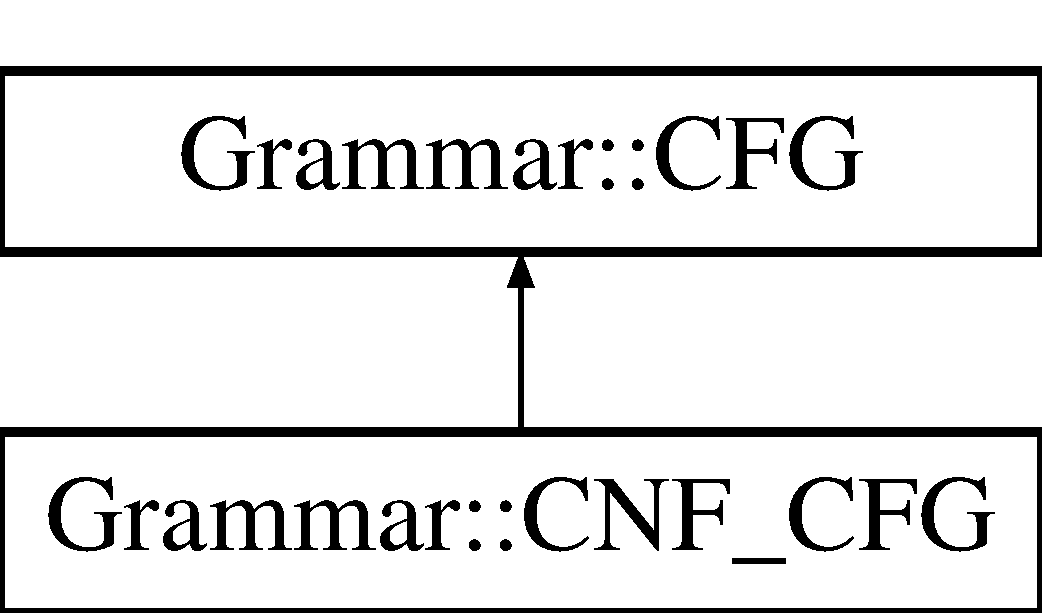
\includegraphics[height=2.000000cm]{dd/dc1/classGrammar_1_1CFG}
\end{center}
\end{figure}
\subsection*{\-Public \-Member \-Functions}
\begin{DoxyCompactItemize}
\item 
\hyperlink{classGrammar_1_1CFG_a2514d591306a5a473cf5fb7526a553fe}{\-C\-F\-G} ()
\begin{DoxyCompactList}\small\item\em \-Default constructor. \end{DoxyCompactList}\item 
\hyperlink{classGrammar_1_1CFG_ac2ad8201bf4de4991d2abcd62f74cddd}{\-C\-F\-G} (std\-::vector$<$ std\-::string $>$ \&v, std\-::vector$<$ std\-::string $>$ \&t, std\-::map$<$ std\-::string, std\-::vector$<$ std\-::string $>$ $>$ \&r, std\-::string s)
\begin{DoxyCompactList}\small\item\em specified constructor \end{DoxyCompactList}\item 
\hyperlink{classGrammar_1_1CFG_aa8d52c4cdfb2a0ef3d1c49148840d333}{\-C\-F\-G} (std\-::string file)
\begin{DoxyCompactList}\small\item\em \-Constructor from a given file. \end{DoxyCompactList}\item 
\hyperlink{classGrammar_1_1CFG_aae4104b0c6f695fa90c2c4a9651b9ac3}{\-C\-F\-G} (\hyperlink{classGrammar_1_1CFG}{\-C\-F\-G} \&copy)
\begin{DoxyCompactList}\small\item\em \-Copy constructor. \end{DoxyCompactList}\item 
void \hyperlink{classGrammar_1_1CFG_ad9c501567ec736260bde8f4076c63a4b}{to\-C\-N\-F} ()
\item 
std\-::vector$<$ std\-::string $>$ \hyperlink{classGrammar_1_1CFG_af0abdc0e7b98c2b735b946261b694ce0}{get\-Variables} () const 
\item 
std\-::vector$<$ std\-::string $>$ \hyperlink{classGrammar_1_1CFG_a4befeaba70b5455e94975670f3d83ba0}{get\-Terminals} () const 
\item 
std\-::map$<$ std\-::string, \*
std\-::vector$<$ std\-::string $>$ $>$ \hyperlink{classGrammar_1_1CFG_a7b964a01cb216bc2c67688724f6058f0}{get\-Rules} () const 
\item 
std\-::string \hyperlink{classGrammar_1_1CFG_a667a1d9eba1917ebe2cd7a63e2d6ffa8}{get\-Start} () const 
\item 
virtual \hyperlink{classGrammar_1_1CFG_a874ad3df12e1f3fd0cd49ad3e9855a45}{$\sim$\-C\-F\-G} ()
\end{DoxyCompactItemize}
\subsection*{\-Protected \-Member \-Functions}
\begin{DoxyCompactItemize}
\item 
void \hyperlink{classGrammar_1_1CFG_af4c1e34192bf5b3e6e26b3240c6502b9}{check\-Attributes} ()
\begin{DoxyCompactList}\small\item\em the start symbol of the \hyperlink{classGrammar_1_1CFG}{\-C\-F\-G} \end{DoxyCompactList}\end{DoxyCompactItemize}
\subsection*{\-Protected \-Attributes}
\begin{DoxyCompactItemize}
\item 
std\-::vector$<$ std\-::string $>$ \hyperlink{classGrammar_1_1CFG_a7041e847818a2e4777bc41d0c2f1db2c}{variables\-\_\-}
\item 
std\-::vector$<$ std\-::string $>$ \hyperlink{classGrammar_1_1CFG_a65298cf1151bb130a382a4858d99a571}{terminals\-\_\-}
\begin{DoxyCompactList}\small\item\em vector with the variables of the \hyperlink{classGrammar_1_1CFG}{\-C\-F\-G} \end{DoxyCompactList}\item 
std\-::map$<$ std\-::string, \*
std\-::vector$<$ std\-::string $>$ $>$ \hyperlink{classGrammar_1_1CFG_a5d91974246061afc53951ef9fac313ad}{rules\-\_\-}
\begin{DoxyCompactList}\small\item\em vector with the terminals of the \hyperlink{classGrammar_1_1CFG}{\-C\-F\-G} \end{DoxyCompactList}\item 
std\-::string \hyperlink{classGrammar_1_1CFG_aaddc2586c72b3f257acf18bf98881623}{start\-Symbol\-\_\-}
\begin{DoxyCompactList}\small\item\em a map with all the rules. rules are of the form $<$\-Variable$>$, vector$<$\-Variables, terminals$>$ \end{DoxyCompactList}\end{DoxyCompactItemize}
\subsection*{\-Friends}
\begin{DoxyCompactItemize}
\item 
std\-::ostream \& \hyperlink{classGrammar_1_1CFG_a125cf827399aa731591064e741ab8fb7}{operator$<$$<$} (std\-::ostream \&out, \hyperlink{classGrammar_1_1CFG}{\-C\-F\-G} \&c)
\begin{DoxyCompactList}\small\item\em output operator \end{DoxyCompactList}\end{DoxyCompactItemize}


\subsection{\-Constructor \& \-Destructor \-Documentation}
\hypertarget{classGrammar_1_1CFG_a2514d591306a5a473cf5fb7526a553fe}{\index{\-Grammar\-::\-C\-F\-G@{\-Grammar\-::\-C\-F\-G}!\-C\-F\-G@{\-C\-F\-G}}
\index{\-C\-F\-G@{\-C\-F\-G}!Grammar::CFG@{\-Grammar\-::\-C\-F\-G}}
\subsubsection[{\-C\-F\-G}]{\setlength{\rightskip}{0pt plus 5cm}{\bf \-Grammar\-::\-C\-F\-G\-::\-C\-F\-G} (
\begin{DoxyParamCaption}
{}
\end{DoxyParamCaption}
)}}\label{dd/dc1/classGrammar_1_1CFG_a2514d591306a5a473cf5fb7526a553fe}


\-Default constructor. 

\hypertarget{classGrammar_1_1CFG_ac2ad8201bf4de4991d2abcd62f74cddd}{\index{\-Grammar\-::\-C\-F\-G@{\-Grammar\-::\-C\-F\-G}!\-C\-F\-G@{\-C\-F\-G}}
\index{\-C\-F\-G@{\-C\-F\-G}!Grammar::CFG@{\-Grammar\-::\-C\-F\-G}}
\subsubsection[{\-C\-F\-G}]{\setlength{\rightskip}{0pt plus 5cm}{\bf \-Grammar\-::\-C\-F\-G\-::\-C\-F\-G} (
\begin{DoxyParamCaption}
\item[{std\-::vector$<$ std\-::string $>$ \&}]{v, }
\item[{std\-::vector$<$ std\-::string $>$ \&}]{t, }
\item[{std\-::map$<$ std\-::string, std\-::vector$<$ std\-::string $>$ $>$ \&}]{r, }
\item[{std\-::string}]{s}
\end{DoxyParamCaption}
)}}\label{dd/dc1/classGrammar_1_1CFG_ac2ad8201bf4de4991d2abcd62f74cddd}


specified constructor 


\begin{DoxyParams}{\-Parameters}
{\em v} & vector with variables \\
\hline
{\em t} & vector with terminals \\
\hline
{\em r} & map with rules of the form $<$\-Variable$>$, vector$<$terminals,\-Variables$>$ \\
\hline
{\em s} & the start symbol for the \hyperlink{classGrammar_1_1CFG}{\-C\-F\-G} \\
\hline
\end{DoxyParams}
\hypertarget{classGrammar_1_1CFG_aa8d52c4cdfb2a0ef3d1c49148840d333}{\index{\-Grammar\-::\-C\-F\-G@{\-Grammar\-::\-C\-F\-G}!\-C\-F\-G@{\-C\-F\-G}}
\index{\-C\-F\-G@{\-C\-F\-G}!Grammar::CFG@{\-Grammar\-::\-C\-F\-G}}
\subsubsection[{\-C\-F\-G}]{\setlength{\rightskip}{0pt plus 5cm}{\bf \-Grammar\-::\-C\-F\-G\-::\-C\-F\-G} (
\begin{DoxyParamCaption}
\item[{std\-::string}]{file}
\end{DoxyParamCaption}
)}}\label{dd/dc1/classGrammar_1_1CFG_aa8d52c4cdfb2a0ef3d1c49148840d333}


\-Constructor from a given file. 


\begin{DoxyParams}{\-Parameters}
{\em file} & the path to a file where the \hyperlink{classGrammar_1_1CFG}{\-C\-F\-G} is described \\
\hline
\end{DoxyParams}
\hypertarget{classGrammar_1_1CFG_aae4104b0c6f695fa90c2c4a9651b9ac3}{\index{\-Grammar\-::\-C\-F\-G@{\-Grammar\-::\-C\-F\-G}!\-C\-F\-G@{\-C\-F\-G}}
\index{\-C\-F\-G@{\-C\-F\-G}!Grammar::CFG@{\-Grammar\-::\-C\-F\-G}}
\subsubsection[{\-C\-F\-G}]{\setlength{\rightskip}{0pt plus 5cm}{\bf \-Grammar\-::\-C\-F\-G\-::\-C\-F\-G} (
\begin{DoxyParamCaption}
\item[{{\bf \-C\-F\-G} \&}]{copy}
\end{DoxyParamCaption}
)}}\label{dd/dc1/classGrammar_1_1CFG_aae4104b0c6f695fa90c2c4a9651b9ac3}


\-Copy constructor. 


\begin{DoxyParams}{\-Parameters}
{\em copy} & a \hyperlink{classGrammar_1_1CFG}{\-C\-F\-G} object which is going to be copied \\
\hline
\end{DoxyParams}
\hypertarget{classGrammar_1_1CFG_a874ad3df12e1f3fd0cd49ad3e9855a45}{\index{\-Grammar\-::\-C\-F\-G@{\-Grammar\-::\-C\-F\-G}!$\sim$\-C\-F\-G@{$\sim$\-C\-F\-G}}
\index{$\sim$\-C\-F\-G@{$\sim$\-C\-F\-G}!Grammar::CFG@{\-Grammar\-::\-C\-F\-G}}
\subsubsection[{$\sim$\-C\-F\-G}]{\setlength{\rightskip}{0pt plus 5cm}virtual {\bf \-Grammar\-::\-C\-F\-G\-::$\sim$\-C\-F\-G} (
\begin{DoxyParamCaption}
{}
\end{DoxyParamCaption}
)\hspace{0.3cm}{\ttfamily  \mbox{[}virtual\mbox{]}}}}\label{dd/dc1/classGrammar_1_1CFG_a874ad3df12e1f3fd0cd49ad3e9855a45}


\subsection{\-Member \-Function \-Documentation}
\hypertarget{classGrammar_1_1CFG_af4c1e34192bf5b3e6e26b3240c6502b9}{\index{\-Grammar\-::\-C\-F\-G@{\-Grammar\-::\-C\-F\-G}!check\-Attributes@{check\-Attributes}}
\index{check\-Attributes@{check\-Attributes}!Grammar::CFG@{\-Grammar\-::\-C\-F\-G}}
\subsubsection[{check\-Attributes}]{\setlength{\rightskip}{0pt plus 5cm}void {\bf \-Grammar\-::\-C\-F\-G\-::check\-Attributes} (
\begin{DoxyParamCaption}
{}
\end{DoxyParamCaption}
)\hspace{0.3cm}{\ttfamily  \mbox{[}protected\mbox{]}}}}\label{dd/dc1/classGrammar_1_1CFG_af4c1e34192bf5b3e6e26b3240c6502b9}


the start symbol of the \hyperlink{classGrammar_1_1CFG}{\-C\-F\-G} 

checks whether all attributes are ok \hypertarget{classGrammar_1_1CFG_a7b964a01cb216bc2c67688724f6058f0}{\index{\-Grammar\-::\-C\-F\-G@{\-Grammar\-::\-C\-F\-G}!get\-Rules@{get\-Rules}}
\index{get\-Rules@{get\-Rules}!Grammar::CFG@{\-Grammar\-::\-C\-F\-G}}
\subsubsection[{get\-Rules}]{\setlength{\rightskip}{0pt plus 5cm}std\-::map$<$std\-::string, std\-::vector$<$std\-::string$>$ $>$ {\bf \-Grammar\-::\-C\-F\-G\-::get\-Rules} (
\begin{DoxyParamCaption}
{}
\end{DoxyParamCaption}
) const}}\label{dd/dc1/classGrammar_1_1CFG_a7b964a01cb216bc2c67688724f6058f0}
\hypertarget{classGrammar_1_1CFG_a667a1d9eba1917ebe2cd7a63e2d6ffa8}{\index{\-Grammar\-::\-C\-F\-G@{\-Grammar\-::\-C\-F\-G}!get\-Start@{get\-Start}}
\index{get\-Start@{get\-Start}!Grammar::CFG@{\-Grammar\-::\-C\-F\-G}}
\subsubsection[{get\-Start}]{\setlength{\rightskip}{0pt plus 5cm}std\-::string {\bf \-Grammar\-::\-C\-F\-G\-::get\-Start} (
\begin{DoxyParamCaption}
{}
\end{DoxyParamCaption}
) const}}\label{dd/dc1/classGrammar_1_1CFG_a667a1d9eba1917ebe2cd7a63e2d6ffa8}
\hypertarget{classGrammar_1_1CFG_a4befeaba70b5455e94975670f3d83ba0}{\index{\-Grammar\-::\-C\-F\-G@{\-Grammar\-::\-C\-F\-G}!get\-Terminals@{get\-Terminals}}
\index{get\-Terminals@{get\-Terminals}!Grammar::CFG@{\-Grammar\-::\-C\-F\-G}}
\subsubsection[{get\-Terminals}]{\setlength{\rightskip}{0pt plus 5cm}std\-::vector$<$std\-::string$>$ {\bf \-Grammar\-::\-C\-F\-G\-::get\-Terminals} (
\begin{DoxyParamCaption}
{}
\end{DoxyParamCaption}
) const}}\label{dd/dc1/classGrammar_1_1CFG_a4befeaba70b5455e94975670f3d83ba0}
\hypertarget{classGrammar_1_1CFG_af0abdc0e7b98c2b735b946261b694ce0}{\index{\-Grammar\-::\-C\-F\-G@{\-Grammar\-::\-C\-F\-G}!get\-Variables@{get\-Variables}}
\index{get\-Variables@{get\-Variables}!Grammar::CFG@{\-Grammar\-::\-C\-F\-G}}
\subsubsection[{get\-Variables}]{\setlength{\rightskip}{0pt plus 5cm}std\-::vector$<$std\-::string$>$ {\bf \-Grammar\-::\-C\-F\-G\-::get\-Variables} (
\begin{DoxyParamCaption}
{}
\end{DoxyParamCaption}
) const}}\label{dd/dc1/classGrammar_1_1CFG_af0abdc0e7b98c2b735b946261b694ce0}
\hypertarget{classGrammar_1_1CFG_ad9c501567ec736260bde8f4076c63a4b}{\index{\-Grammar\-::\-C\-F\-G@{\-Grammar\-::\-C\-F\-G}!to\-C\-N\-F@{to\-C\-N\-F}}
\index{to\-C\-N\-F@{to\-C\-N\-F}!Grammar::CFG@{\-Grammar\-::\-C\-F\-G}}
\subsubsection[{to\-C\-N\-F}]{\setlength{\rightskip}{0pt plus 5cm}void {\bf \-Grammar\-::\-C\-F\-G\-::to\-C\-N\-F} (
\begin{DoxyParamCaption}
{}
\end{DoxyParamCaption}
)}}\label{dd/dc1/classGrammar_1_1CFG_ad9c501567ec736260bde8f4076c63a4b}


\subsection{\-Friends \-And \-Related \-Function \-Documentation}
\hypertarget{classGrammar_1_1CFG_a125cf827399aa731591064e741ab8fb7}{\index{\-Grammar\-::\-C\-F\-G@{\-Grammar\-::\-C\-F\-G}!operator$<$$<$@{operator$<$$<$}}
\index{operator$<$$<$@{operator$<$$<$}!Grammar::CFG@{\-Grammar\-::\-C\-F\-G}}
\subsubsection[{operator$<$$<$}]{\setlength{\rightskip}{0pt plus 5cm}std\-::ostream\& operator$<$$<$ (
\begin{DoxyParamCaption}
\item[{std\-::ostream \&}]{out, }
\item[{{\bf \-C\-F\-G} \&}]{c}
\end{DoxyParamCaption}
)\hspace{0.3cm}{\ttfamily  \mbox{[}friend\mbox{]}}}}\label{dd/dc1/classGrammar_1_1CFG_a125cf827399aa731591064e741ab8fb7}


output operator 



\subsection{\-Member \-Data \-Documentation}
\hypertarget{classGrammar_1_1CFG_a5d91974246061afc53951ef9fac313ad}{\index{\-Grammar\-::\-C\-F\-G@{\-Grammar\-::\-C\-F\-G}!rules\-\_\-@{rules\-\_\-}}
\index{rules\-\_\-@{rules\-\_\-}!Grammar::CFG@{\-Grammar\-::\-C\-F\-G}}
\subsubsection[{rules\-\_\-}]{\setlength{\rightskip}{0pt plus 5cm}std\-::map$<$std\-::string, std\-::vector$<$std\-::string$>$ $>$ {\bf \-Grammar\-::\-C\-F\-G\-::rules\-\_\-}\hspace{0.3cm}{\ttfamily  \mbox{[}protected\mbox{]}}}}\label{dd/dc1/classGrammar_1_1CFG_a5d91974246061afc53951ef9fac313ad}


vector with the terminals of the \hyperlink{classGrammar_1_1CFG}{\-C\-F\-G} 

\hypertarget{classGrammar_1_1CFG_aaddc2586c72b3f257acf18bf98881623}{\index{\-Grammar\-::\-C\-F\-G@{\-Grammar\-::\-C\-F\-G}!start\-Symbol\-\_\-@{start\-Symbol\-\_\-}}
\index{start\-Symbol\-\_\-@{start\-Symbol\-\_\-}!Grammar::CFG@{\-Grammar\-::\-C\-F\-G}}
\subsubsection[{start\-Symbol\-\_\-}]{\setlength{\rightskip}{0pt plus 5cm}std\-::string {\bf \-Grammar\-::\-C\-F\-G\-::start\-Symbol\-\_\-}\hspace{0.3cm}{\ttfamily  \mbox{[}protected\mbox{]}}}}\label{dd/dc1/classGrammar_1_1CFG_aaddc2586c72b3f257acf18bf98881623}


a map with all the rules. rules are of the form $<$\-Variable$>$, vector$<$\-Variables, terminals$>$ 

\hypertarget{classGrammar_1_1CFG_a65298cf1151bb130a382a4858d99a571}{\index{\-Grammar\-::\-C\-F\-G@{\-Grammar\-::\-C\-F\-G}!terminals\-\_\-@{terminals\-\_\-}}
\index{terminals\-\_\-@{terminals\-\_\-}!Grammar::CFG@{\-Grammar\-::\-C\-F\-G}}
\subsubsection[{terminals\-\_\-}]{\setlength{\rightskip}{0pt plus 5cm}std\-::vector$<$std\-::string$>$ {\bf \-Grammar\-::\-C\-F\-G\-::terminals\-\_\-}\hspace{0.3cm}{\ttfamily  \mbox{[}protected\mbox{]}}}}\label{dd/dc1/classGrammar_1_1CFG_a65298cf1151bb130a382a4858d99a571}


vector with the variables of the \hyperlink{classGrammar_1_1CFG}{\-C\-F\-G} 

\hypertarget{classGrammar_1_1CFG_a7041e847818a2e4777bc41d0c2f1db2c}{\index{\-Grammar\-::\-C\-F\-G@{\-Grammar\-::\-C\-F\-G}!variables\-\_\-@{variables\-\_\-}}
\index{variables\-\_\-@{variables\-\_\-}!Grammar::CFG@{\-Grammar\-::\-C\-F\-G}}
\subsubsection[{variables\-\_\-}]{\setlength{\rightskip}{0pt plus 5cm}std\-::vector$<$std\-::string$>$ {\bf \-Grammar\-::\-C\-F\-G\-::variables\-\_\-}\hspace{0.3cm}{\ttfamily  \mbox{[}protected\mbox{]}}}}\label{dd/dc1/classGrammar_1_1CFG_a7041e847818a2e4777bc41d0c2f1db2c}


\-The documentation for this class was generated from the following file\-:\begin{DoxyCompactItemize}
\item 
src/\hyperlink{CFG_8h}{\-C\-F\-G.\-h}\end{DoxyCompactItemize}

\hypertarget{classparser_1_1CFGParser}{\section{parser\-:\-:\-C\-F\-G\-Parser \-Class \-Reference}
\label{de/d63/classparser_1_1CFGParser}\index{parser\-::\-C\-F\-G\-Parser@{parser\-::\-C\-F\-G\-Parser}}
}


{\ttfamily \#include $<$\-Parser.\-h$>$}

\-Inheritance diagram for parser\-:\-:\-C\-F\-G\-Parser\-:\begin{figure}[H]
\begin{center}
\leavevmode
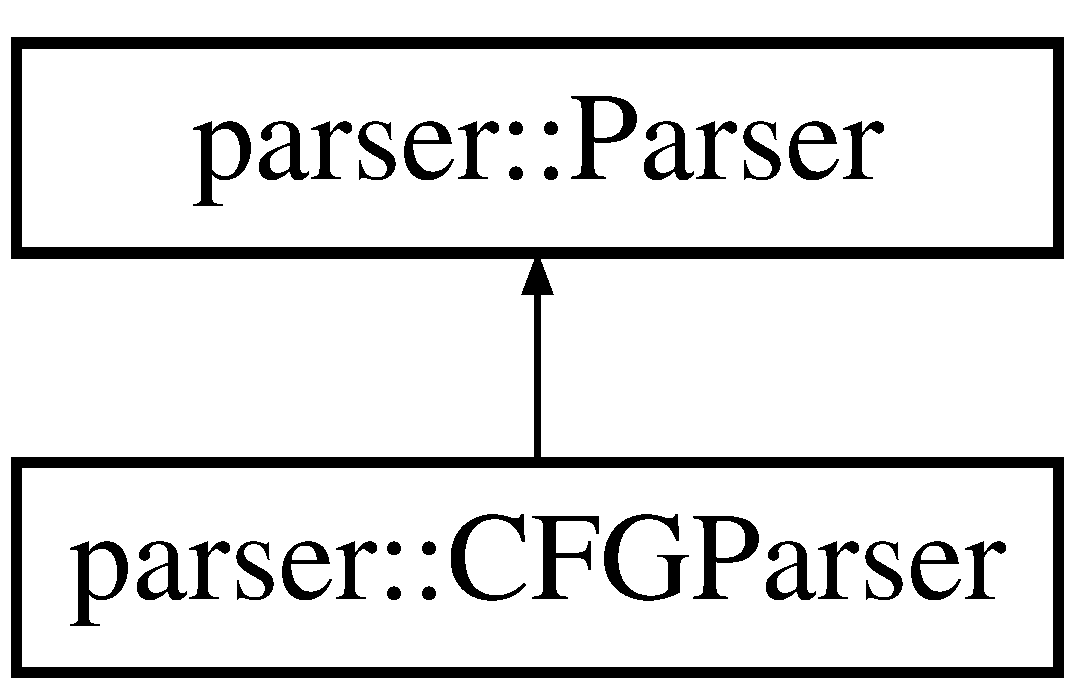
\includegraphics[height=2.000000cm]{de/d63/classparser_1_1CFGParser}
\end{center}
\end{figure}
\subsection*{\-Public \-Member \-Functions}
\begin{DoxyCompactItemize}
\item 
\hyperlink{classparser_1_1CFGParser_adfc299d4c11f48a08c27c4e07a11d3ef}{\-C\-F\-G\-Parser} (std\-::string)
\begin{DoxyCompactList}\small\item\em \-Default constructor\-: will parse the entire \-C\-F\-G. \end{DoxyCompactList}\item 
virtual \hyperlink{classparser_1_1CFGParser_af49c545d6ff832401e91d0e10c6e3d39}{$\sim$\-C\-F\-G\-Parser} ()
\item 
std\-::vector$<$ std\-::string $>$ \hyperlink{classparser_1_1CFGParser_aa8200b6b3e2e1e2e39d00c3067993c32}{get\-Variables} () const 
\begin{DoxyCompactList}\small\item\em \-Returns the \-C\-F\-G variables. \end{DoxyCompactList}\item 
std\-::vector$<$ std\-::string $>$ \hyperlink{classparser_1_1CFGParser_a6bef668d8312ae21bd194c57cc27ad6b}{get\-Terminals} () const 
\begin{DoxyCompactList}\small\item\em \-Returns the \-C\-F\-G terminals. \end{DoxyCompactList}\item 
std\-::map$<$ std\-::string, \*
std\-::vector$<$ std\-::string $>$ $>$ \hyperlink{classparser_1_1CFGParser_ab1cb8d295814c86d938ef4de7d626b37}{get\-Rules} () const 
\begin{DoxyCompactList}\small\item\em \-Returns the \-C\-F\-G rules. \end{DoxyCompactList}\item 
std\-::string \hyperlink{classparser_1_1CFGParser_a76cc197ff3c26f119032896b0099322e}{get\-Start} () const 
\begin{DoxyCompactList}\small\item\em \-Returns the start of the \-C\-F\-G. \end{DoxyCompactList}\end{DoxyCompactItemize}
\subsection*{\-Private \-Member \-Functions}
\begin{DoxyCompactItemize}
\item 
void \hyperlink{classparser_1_1CFGParser_a8825f263a7d78ca9ea3e1975dca5a22e}{parse\-Variables} (\-Ti\-Xml\-Element $\ast$)
\begin{DoxyCompactList}\small\item\em \-Parses the variables of the \-C\-F\-G. \end{DoxyCompactList}\item 
void \hyperlink{classparser_1_1CFGParser_adc9127ccdb636a5a05e78b3f1fc8b9fa}{parse\-Terminals} (\-Ti\-Xml\-Element $\ast$)
\begin{DoxyCompactList}\small\item\em \-Parses the terminals of the \-C\-F\-G. \end{DoxyCompactList}\item 
void \hyperlink{classparser_1_1CFGParser_a800e4c71a5666661aa27497f190ea77e}{parse\-Rules} (\-Ti\-Xml\-Element $\ast$)
\begin{DoxyCompactList}\small\item\em \-Parses the rules of the \-C\-F\-G. \end{DoxyCompactList}\item 
void \hyperlink{classparser_1_1CFGParser_a2015d0db934eb8cceb8f236017c49469}{parse\-Start} (\-Ti\-Xml\-Element $\ast$)
\begin{DoxyCompactList}\small\item\em \-Parses the start symbol of the \-C\-F\-G. \end{DoxyCompactList}\end{DoxyCompactItemize}
\subsection*{\-Private \-Attributes}
\begin{DoxyCompactItemize}
\item 
std\-::vector$<$ std\-::string $>$ \hyperlink{classparser_1_1CFGParser_a683c57ac6f377ad4fa4c074df294ee4d}{variables}
\item 
std\-::vector$<$ std\-::string $>$ \hyperlink{classparser_1_1CFGParser_a5709544c0a9981997043f38489f2ddff}{terminals}
\item 
std\-::map$<$ std\-::string, \*
std\-::vector$<$ std\-::string $>$ $>$ \hyperlink{classparser_1_1CFGParser_a2848eb1b568b538e2f49d237cd32351d}{rules}
\item 
std\-::string \hyperlink{classparser_1_1CFGParser_a6d3a8eefa11cca703d7126031c59d220}{start\-Symbol}
\end{DoxyCompactItemize}


\subsection{\-Constructor \& \-Destructor \-Documentation}
\hypertarget{classparser_1_1CFGParser_adfc299d4c11f48a08c27c4e07a11d3ef}{\index{parser\-::\-C\-F\-G\-Parser@{parser\-::\-C\-F\-G\-Parser}!\-C\-F\-G\-Parser@{\-C\-F\-G\-Parser}}
\index{\-C\-F\-G\-Parser@{\-C\-F\-G\-Parser}!parser::CFGParser@{parser\-::\-C\-F\-G\-Parser}}
\subsubsection[{\-C\-F\-G\-Parser}]{\setlength{\rightskip}{0pt plus 5cm}{\bf parser\-::\-C\-F\-G\-Parser\-::\-C\-F\-G\-Parser} (
\begin{DoxyParamCaption}
\item[{std\-::string}]{}
\end{DoxyParamCaption}
)}}\label{de/d63/classparser_1_1CFGParser_adfc299d4c11f48a08c27c4e07a11d3ef}


\-Default constructor\-: will parse the entire \-C\-F\-G. 


\begin{DoxyParams}{\-Parameters}
{\em filename} & \-X\-M\-L file that describes the to be parsed \-C\-F\-G. \\
\hline
\end{DoxyParams}
\hypertarget{classparser_1_1CFGParser_af49c545d6ff832401e91d0e10c6e3d39}{\index{parser\-::\-C\-F\-G\-Parser@{parser\-::\-C\-F\-G\-Parser}!$\sim$\-C\-F\-G\-Parser@{$\sim$\-C\-F\-G\-Parser}}
\index{$\sim$\-C\-F\-G\-Parser@{$\sim$\-C\-F\-G\-Parser}!parser::CFGParser@{parser\-::\-C\-F\-G\-Parser}}
\subsubsection[{$\sim$\-C\-F\-G\-Parser}]{\setlength{\rightskip}{0pt plus 5cm}virtual {\bf parser\-::\-C\-F\-G\-Parser\-::$\sim$\-C\-F\-G\-Parser} (
\begin{DoxyParamCaption}
{}
\end{DoxyParamCaption}
)\hspace{0.3cm}{\ttfamily  \mbox{[}virtual\mbox{]}}}}\label{de/d63/classparser_1_1CFGParser_af49c545d6ff832401e91d0e10c6e3d39}


\subsection{\-Member \-Function \-Documentation}
\hypertarget{classparser_1_1CFGParser_ab1cb8d295814c86d938ef4de7d626b37}{\index{parser\-::\-C\-F\-G\-Parser@{parser\-::\-C\-F\-G\-Parser}!get\-Rules@{get\-Rules}}
\index{get\-Rules@{get\-Rules}!parser::CFGParser@{parser\-::\-C\-F\-G\-Parser}}
\subsubsection[{get\-Rules}]{\setlength{\rightskip}{0pt plus 5cm}std\-::map$<$std\-::string, std\-::vector$<$std\-::string$>$ $>$ {\bf parser\-::\-C\-F\-G\-Parser\-::get\-Rules} (
\begin{DoxyParamCaption}
{}
\end{DoxyParamCaption}
) const}}\label{de/d63/classparser_1_1CFGParser_ab1cb8d295814c86d938ef4de7d626b37}


\-Returns the \-C\-F\-G rules. 

\begin{DoxyReturn}{\-Returns}
\-A map in the form of (head, body) 
\end{DoxyReturn}
\hypertarget{classparser_1_1CFGParser_a76cc197ff3c26f119032896b0099322e}{\index{parser\-::\-C\-F\-G\-Parser@{parser\-::\-C\-F\-G\-Parser}!get\-Start@{get\-Start}}
\index{get\-Start@{get\-Start}!parser::CFGParser@{parser\-::\-C\-F\-G\-Parser}}
\subsubsection[{get\-Start}]{\setlength{\rightskip}{0pt plus 5cm}std\-::string {\bf parser\-::\-C\-F\-G\-Parser\-::get\-Start} (
\begin{DoxyParamCaption}
{}
\end{DoxyParamCaption}
) const}}\label{de/d63/classparser_1_1CFGParser_a76cc197ff3c26f119032896b0099322e}


\-Returns the start of the \-C\-F\-G. 

\begin{DoxyReturn}{\-Returns}
\-The start variable (string) 
\end{DoxyReturn}
\hypertarget{classparser_1_1CFGParser_a6bef668d8312ae21bd194c57cc27ad6b}{\index{parser\-::\-C\-F\-G\-Parser@{parser\-::\-C\-F\-G\-Parser}!get\-Terminals@{get\-Terminals}}
\index{get\-Terminals@{get\-Terminals}!parser::CFGParser@{parser\-::\-C\-F\-G\-Parser}}
\subsubsection[{get\-Terminals}]{\setlength{\rightskip}{0pt plus 5cm}std\-::vector$<$std\-::string$>$ {\bf parser\-::\-C\-F\-G\-Parser\-::get\-Terminals} (
\begin{DoxyParamCaption}
{}
\end{DoxyParamCaption}
) const}}\label{de/d63/classparser_1_1CFGParser_a6bef668d8312ae21bd194c57cc27ad6b}


\-Returns the \-C\-F\-G terminals. 

\begin{DoxyReturn}{\-Returns}
\-A vector containing the terminals (strings). 
\end{DoxyReturn}
\hypertarget{classparser_1_1CFGParser_aa8200b6b3e2e1e2e39d00c3067993c32}{\index{parser\-::\-C\-F\-G\-Parser@{parser\-::\-C\-F\-G\-Parser}!get\-Variables@{get\-Variables}}
\index{get\-Variables@{get\-Variables}!parser::CFGParser@{parser\-::\-C\-F\-G\-Parser}}
\subsubsection[{get\-Variables}]{\setlength{\rightskip}{0pt plus 5cm}std\-::vector$<$std\-::string$>$ {\bf parser\-::\-C\-F\-G\-Parser\-::get\-Variables} (
\begin{DoxyParamCaption}
{}
\end{DoxyParamCaption}
) const}}\label{de/d63/classparser_1_1CFGParser_aa8200b6b3e2e1e2e39d00c3067993c32}


\-Returns the \-C\-F\-G variables. 

\begin{DoxyReturn}{\-Returns}
\-A vector containing the variables (strings). 
\end{DoxyReturn}
\hypertarget{classparser_1_1CFGParser_a800e4c71a5666661aa27497f190ea77e}{\index{parser\-::\-C\-F\-G\-Parser@{parser\-::\-C\-F\-G\-Parser}!parse\-Rules@{parse\-Rules}}
\index{parse\-Rules@{parse\-Rules}!parser::CFGParser@{parser\-::\-C\-F\-G\-Parser}}
\subsubsection[{parse\-Rules}]{\setlength{\rightskip}{0pt plus 5cm}void {\bf parser\-::\-C\-F\-G\-Parser\-::parse\-Rules} (
\begin{DoxyParamCaption}
\item[{\-Ti\-Xml\-Element $\ast$}]{}
\end{DoxyParamCaption}
)\hspace{0.3cm}{\ttfamily  \mbox{[}private\mbox{]}}}}\label{de/d63/classparser_1_1CFGParser_a800e4c71a5666661aa27497f190ea77e}


\-Parses the rules of the \-C\-F\-G. 

\hypertarget{classparser_1_1CFGParser_a2015d0db934eb8cceb8f236017c49469}{\index{parser\-::\-C\-F\-G\-Parser@{parser\-::\-C\-F\-G\-Parser}!parse\-Start@{parse\-Start}}
\index{parse\-Start@{parse\-Start}!parser::CFGParser@{parser\-::\-C\-F\-G\-Parser}}
\subsubsection[{parse\-Start}]{\setlength{\rightskip}{0pt plus 5cm}void {\bf parser\-::\-C\-F\-G\-Parser\-::parse\-Start} (
\begin{DoxyParamCaption}
\item[{\-Ti\-Xml\-Element $\ast$}]{}
\end{DoxyParamCaption}
)\hspace{0.3cm}{\ttfamily  \mbox{[}private\mbox{]}}}}\label{de/d63/classparser_1_1CFGParser_a2015d0db934eb8cceb8f236017c49469}


\-Parses the start symbol of the \-C\-F\-G. 

\hypertarget{classparser_1_1CFGParser_adc9127ccdb636a5a05e78b3f1fc8b9fa}{\index{parser\-::\-C\-F\-G\-Parser@{parser\-::\-C\-F\-G\-Parser}!parse\-Terminals@{parse\-Terminals}}
\index{parse\-Terminals@{parse\-Terminals}!parser::CFGParser@{parser\-::\-C\-F\-G\-Parser}}
\subsubsection[{parse\-Terminals}]{\setlength{\rightskip}{0pt plus 5cm}void {\bf parser\-::\-C\-F\-G\-Parser\-::parse\-Terminals} (
\begin{DoxyParamCaption}
\item[{\-Ti\-Xml\-Element $\ast$}]{}
\end{DoxyParamCaption}
)\hspace{0.3cm}{\ttfamily  \mbox{[}private\mbox{]}}}}\label{de/d63/classparser_1_1CFGParser_adc9127ccdb636a5a05e78b3f1fc8b9fa}


\-Parses the terminals of the \-C\-F\-G. 

\hypertarget{classparser_1_1CFGParser_a8825f263a7d78ca9ea3e1975dca5a22e}{\index{parser\-::\-C\-F\-G\-Parser@{parser\-::\-C\-F\-G\-Parser}!parse\-Variables@{parse\-Variables}}
\index{parse\-Variables@{parse\-Variables}!parser::CFGParser@{parser\-::\-C\-F\-G\-Parser}}
\subsubsection[{parse\-Variables}]{\setlength{\rightskip}{0pt plus 5cm}void {\bf parser\-::\-C\-F\-G\-Parser\-::parse\-Variables} (
\begin{DoxyParamCaption}
\item[{\-Ti\-Xml\-Element $\ast$}]{}
\end{DoxyParamCaption}
)\hspace{0.3cm}{\ttfamily  \mbox{[}private\mbox{]}}}}\label{de/d63/classparser_1_1CFGParser_a8825f263a7d78ca9ea3e1975dca5a22e}


\-Parses the variables of the \-C\-F\-G. 



\subsection{\-Member \-Data \-Documentation}
\hypertarget{classparser_1_1CFGParser_a2848eb1b568b538e2f49d237cd32351d}{\index{parser\-::\-C\-F\-G\-Parser@{parser\-::\-C\-F\-G\-Parser}!rules@{rules}}
\index{rules@{rules}!parser::CFGParser@{parser\-::\-C\-F\-G\-Parser}}
\subsubsection[{rules}]{\setlength{\rightskip}{0pt plus 5cm}std\-::map$<$std\-::string, std\-::vector$<$std\-::string$>$ $>$ {\bf parser\-::\-C\-F\-G\-Parser\-::rules}\hspace{0.3cm}{\ttfamily  \mbox{[}private\mbox{]}}}}\label{de/d63/classparser_1_1CFGParser_a2848eb1b568b538e2f49d237cd32351d}
\hypertarget{classparser_1_1CFGParser_a6d3a8eefa11cca703d7126031c59d220}{\index{parser\-::\-C\-F\-G\-Parser@{parser\-::\-C\-F\-G\-Parser}!start\-Symbol@{start\-Symbol}}
\index{start\-Symbol@{start\-Symbol}!parser::CFGParser@{parser\-::\-C\-F\-G\-Parser}}
\subsubsection[{start\-Symbol}]{\setlength{\rightskip}{0pt plus 5cm}std\-::string {\bf parser\-::\-C\-F\-G\-Parser\-::start\-Symbol}\hspace{0.3cm}{\ttfamily  \mbox{[}private\mbox{]}}}}\label{de/d63/classparser_1_1CFGParser_a6d3a8eefa11cca703d7126031c59d220}
\hypertarget{classparser_1_1CFGParser_a5709544c0a9981997043f38489f2ddff}{\index{parser\-::\-C\-F\-G\-Parser@{parser\-::\-C\-F\-G\-Parser}!terminals@{terminals}}
\index{terminals@{terminals}!parser::CFGParser@{parser\-::\-C\-F\-G\-Parser}}
\subsubsection[{terminals}]{\setlength{\rightskip}{0pt plus 5cm}std\-::vector$<$std\-::string$>$ {\bf parser\-::\-C\-F\-G\-Parser\-::terminals}\hspace{0.3cm}{\ttfamily  \mbox{[}private\mbox{]}}}}\label{de/d63/classparser_1_1CFGParser_a5709544c0a9981997043f38489f2ddff}
\hypertarget{classparser_1_1CFGParser_a683c57ac6f377ad4fa4c074df294ee4d}{\index{parser\-::\-C\-F\-G\-Parser@{parser\-::\-C\-F\-G\-Parser}!variables@{variables}}
\index{variables@{variables}!parser::CFGParser@{parser\-::\-C\-F\-G\-Parser}}
\subsubsection[{variables}]{\setlength{\rightskip}{0pt plus 5cm}std\-::vector$<$std\-::string$>$ {\bf parser\-::\-C\-F\-G\-Parser\-::variables}\hspace{0.3cm}{\ttfamily  \mbox{[}private\mbox{]}}}}\label{de/d63/classparser_1_1CFGParser_a683c57ac6f377ad4fa4c074df294ee4d}


\-The documentation for this class was generated from the following file\-:\begin{DoxyCompactItemize}
\item 
src/\hyperlink{Parser_8h}{\-Parser.\-h}\end{DoxyCompactItemize}

\hypertarget{classGrammar_1_1CNF__CFG}{\section{\-Grammar\-:\-:\-C\-N\-F\-\_\-\-C\-F\-G \-Class \-Reference}
\label{dc/d05/classGrammar_1_1CNF__CFG}\index{\-Grammar\-::\-C\-N\-F\-\_\-\-C\-F\-G@{\-Grammar\-::\-C\-N\-F\-\_\-\-C\-F\-G}}
}


{\ttfamily \#include $<$\-C\-F\-G.\-h$>$}

\-Inheritance diagram for \-Grammar\-:\-:\-C\-N\-F\-\_\-\-C\-F\-G\-:\begin{figure}[H]
\begin{center}
\leavevmode
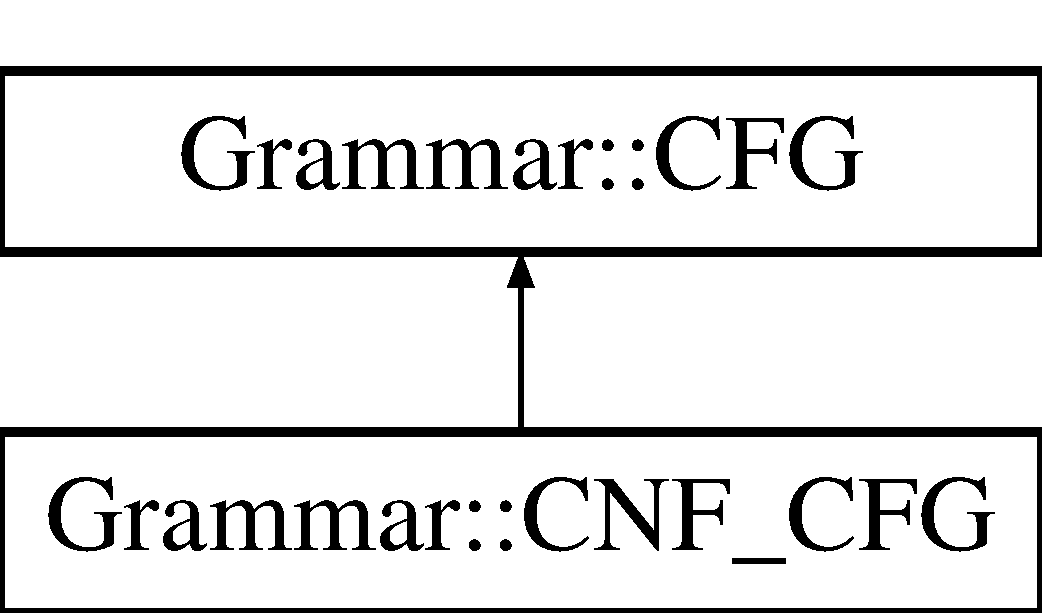
\includegraphics[height=2.000000cm]{dc/d05/classGrammar_1_1CNF__CFG}
\end{center}
\end{figure}
\subsection*{\-Public \-Member \-Functions}
\begin{DoxyCompactItemize}
\item 
\hyperlink{classGrammar_1_1CNF__CFG_aa5850ca203f633fb16b4c74ea50e25f8}{\-C\-N\-F\-\_\-\-C\-F\-G} ()
\begin{DoxyCompactList}\small\item\em \-Default constructor. \end{DoxyCompactList}\item 
\hyperlink{classGrammar_1_1CNF__CFG_a9526886948355942d078fc55e69e73c7}{\-C\-N\-F\-\_\-\-C\-F\-G} (std\-::vector$<$ std\-::string $>$ \&v, std\-::vector$<$ std\-::string $>$ \&t, std\-::map$<$ std\-::string, std\-::vector$<$ std\-::string $>$ $>$ \&r, std\-::string s)
\begin{DoxyCompactList}\small\item\em specified constructor \end{DoxyCompactList}\item 
\hyperlink{classGrammar_1_1CNF__CFG_a88865800e932d5c81dae48d1be25adb7}{\-C\-N\-F\-\_\-\-C\-F\-G} (\hyperlink{classGrammar_1_1CFG}{\-C\-F\-G} \&cfg)
\begin{DoxyCompactList}\small\item\em constructor based on a \hyperlink{classGrammar_1_1CFG}{\-C\-F\-G} and copy constructor \end{DoxyCompactList}\item 
\hyperlink{classGrammar_1_1CNF__CFG_a90ddda4519a646b86ce74e5f7c66af1a}{\-C\-N\-F\-\_\-\-C\-F\-G} (std\-::string file)
\begin{DoxyCompactList}\small\item\em constructor with information file \end{DoxyCompactList}\item 
bool \hyperlink{classGrammar_1_1CNF__CFG_a446adcd68552aec1ee08f7058ac1c1e4}{check\-\_\-string} (std\-::string w)
\begin{DoxyCompactList}\small\item\em checks if given string is in the \hyperlink{classGrammar_1_1CNF__CFG}{\-C\-N\-F\-\_\-\-C\-F\-G} \end{DoxyCompactList}\item 
bool \hyperlink{classGrammar_1_1CNF__CFG_a55bd1300252f9c6bd506ae43738b7616}{already\-\_\-checked} (std\-::string w)
\begin{DoxyCompactList}\small\item\em function used for testing \end{DoxyCompactList}\end{DoxyCompactItemize}
\subsection*{\-Protected \-Member \-Functions}
\begin{DoxyCompactItemize}
\item 
void \hyperlink{classGrammar_1_1CNF__CFG_a541e366bbd28560401f54781425d0954}{check\-Rules} ()
\begin{DoxyCompactList}\small\item\em map keeps track of all the strings that have already been checked on this \hyperlink{classGrammar_1_1CFG}{\-C\-F\-G} with the \-C\-Y\-K algorithm \end{DoxyCompactList}\end{DoxyCompactItemize}
\subsection*{\-Protected \-Attributes}
\begin{DoxyCompactItemize}
\item 
\hyperlink{classGrammar_1_1CYKTable}{\-C\-Y\-K\-Table} \hyperlink{classGrammar_1_1CNF__CFG_ae65bc2d3253161b23e6cdbfc6a40a475}{cyk\-\_\-}
\item 
std\-::map$<$ std\-::string, bool $>$ \hyperlink{classGrammar_1_1CNF__CFG_abb38d3a65837a1d8cf85e3b0e7a1cf15}{checked}
\begin{DoxyCompactList}\small\item\em used to check if given string is in \hyperlink{classGrammar_1_1CFG}{\-C\-F\-G} \end{DoxyCompactList}\end{DoxyCompactItemize}


\subsection{\-Constructor \& \-Destructor \-Documentation}
\hypertarget{classGrammar_1_1CNF__CFG_aa5850ca203f633fb16b4c74ea50e25f8}{\index{\-Grammar\-::\-C\-N\-F\-\_\-\-C\-F\-G@{\-Grammar\-::\-C\-N\-F\-\_\-\-C\-F\-G}!\-C\-N\-F\-\_\-\-C\-F\-G@{\-C\-N\-F\-\_\-\-C\-F\-G}}
\index{\-C\-N\-F\-\_\-\-C\-F\-G@{\-C\-N\-F\-\_\-\-C\-F\-G}!Grammar::CNF_CFG@{\-Grammar\-::\-C\-N\-F\-\_\-\-C\-F\-G}}
\subsubsection[{\-C\-N\-F\-\_\-\-C\-F\-G}]{\setlength{\rightskip}{0pt plus 5cm}{\bf \-Grammar\-::\-C\-N\-F\-\_\-\-C\-F\-G\-::\-C\-N\-F\-\_\-\-C\-F\-G} (
\begin{DoxyParamCaption}
{}
\end{DoxyParamCaption}
)}}\label{dc/d05/classGrammar_1_1CNF__CFG_aa5850ca203f633fb16b4c74ea50e25f8}


\-Default constructor. 

\hypertarget{classGrammar_1_1CNF__CFG_a9526886948355942d078fc55e69e73c7}{\index{\-Grammar\-::\-C\-N\-F\-\_\-\-C\-F\-G@{\-Grammar\-::\-C\-N\-F\-\_\-\-C\-F\-G}!\-C\-N\-F\-\_\-\-C\-F\-G@{\-C\-N\-F\-\_\-\-C\-F\-G}}
\index{\-C\-N\-F\-\_\-\-C\-F\-G@{\-C\-N\-F\-\_\-\-C\-F\-G}!Grammar::CNF_CFG@{\-Grammar\-::\-C\-N\-F\-\_\-\-C\-F\-G}}
\subsubsection[{\-C\-N\-F\-\_\-\-C\-F\-G}]{\setlength{\rightskip}{0pt plus 5cm}{\bf \-Grammar\-::\-C\-N\-F\-\_\-\-C\-F\-G\-::\-C\-N\-F\-\_\-\-C\-F\-G} (
\begin{DoxyParamCaption}
\item[{std\-::vector$<$ std\-::string $>$ \&}]{v, }
\item[{std\-::vector$<$ std\-::string $>$ \&}]{t, }
\item[{std\-::map$<$ std\-::string, std\-::vector$<$ std\-::string $>$ $>$ \&}]{r, }
\item[{std\-::string}]{s}
\end{DoxyParamCaption}
)}}\label{dc/d05/classGrammar_1_1CNF__CFG_a9526886948355942d078fc55e69e73c7}


specified constructor 


\begin{DoxyParams}{\-Parameters}
{\em v} & vector with variables \\
\hline
{\em t} & vector with terminals \\
\hline
{\em r} & map with rules of the form $<$\-Variable$>$, vector$<$terminals,\-Variables$>$ \\
\hline
{\em s} & the start symbol for the \hyperlink{classGrammar_1_1CFG}{\-C\-F\-G} \\
\hline
\end{DoxyParams}
\hypertarget{classGrammar_1_1CNF__CFG_a88865800e932d5c81dae48d1be25adb7}{\index{\-Grammar\-::\-C\-N\-F\-\_\-\-C\-F\-G@{\-Grammar\-::\-C\-N\-F\-\_\-\-C\-F\-G}!\-C\-N\-F\-\_\-\-C\-F\-G@{\-C\-N\-F\-\_\-\-C\-F\-G}}
\index{\-C\-N\-F\-\_\-\-C\-F\-G@{\-C\-N\-F\-\_\-\-C\-F\-G}!Grammar::CNF_CFG@{\-Grammar\-::\-C\-N\-F\-\_\-\-C\-F\-G}}
\subsubsection[{\-C\-N\-F\-\_\-\-C\-F\-G}]{\setlength{\rightskip}{0pt plus 5cm}{\bf \-Grammar\-::\-C\-N\-F\-\_\-\-C\-F\-G\-::\-C\-N\-F\-\_\-\-C\-F\-G} (
\begin{DoxyParamCaption}
\item[{{\bf \-C\-F\-G} \&}]{cfg}
\end{DoxyParamCaption}
)}}\label{dc/d05/classGrammar_1_1CNF__CFG_a88865800e932d5c81dae48d1be25adb7}


constructor based on a \hyperlink{classGrammar_1_1CFG}{\-C\-F\-G} and copy constructor 


\begin{DoxyParams}{\-Parameters}
{\em cfg} & a \hyperlink{classGrammar_1_1CFG}{\-C\-F\-G} that is in \-C\-N\-F form or a \hyperlink{classGrammar_1_1CNF__CFG}{\-C\-N\-F\-\_\-\-C\-F\-G} \\
\hline
\end{DoxyParams}
\hypertarget{classGrammar_1_1CNF__CFG_a90ddda4519a646b86ce74e5f7c66af1a}{\index{\-Grammar\-::\-C\-N\-F\-\_\-\-C\-F\-G@{\-Grammar\-::\-C\-N\-F\-\_\-\-C\-F\-G}!\-C\-N\-F\-\_\-\-C\-F\-G@{\-C\-N\-F\-\_\-\-C\-F\-G}}
\index{\-C\-N\-F\-\_\-\-C\-F\-G@{\-C\-N\-F\-\_\-\-C\-F\-G}!Grammar::CNF_CFG@{\-Grammar\-::\-C\-N\-F\-\_\-\-C\-F\-G}}
\subsubsection[{\-C\-N\-F\-\_\-\-C\-F\-G}]{\setlength{\rightskip}{0pt plus 5cm}{\bf \-Grammar\-::\-C\-N\-F\-\_\-\-C\-F\-G\-::\-C\-N\-F\-\_\-\-C\-F\-G} (
\begin{DoxyParamCaption}
\item[{std\-::string}]{file}
\end{DoxyParamCaption}
)}}\label{dc/d05/classGrammar_1_1CNF__CFG_a90ddda4519a646b86ce74e5f7c66af1a}


constructor with information file 



\subsection{\-Member \-Function \-Documentation}
\hypertarget{classGrammar_1_1CNF__CFG_a55bd1300252f9c6bd506ae43738b7616}{\index{\-Grammar\-::\-C\-N\-F\-\_\-\-C\-F\-G@{\-Grammar\-::\-C\-N\-F\-\_\-\-C\-F\-G}!already\-\_\-checked@{already\-\_\-checked}}
\index{already\-\_\-checked@{already\-\_\-checked}!Grammar::CNF_CFG@{\-Grammar\-::\-C\-N\-F\-\_\-\-C\-F\-G}}
\subsubsection[{already\-\_\-checked}]{\setlength{\rightskip}{0pt plus 5cm}bool {\bf \-Grammar\-::\-C\-N\-F\-\_\-\-C\-F\-G\-::already\-\_\-checked} (
\begin{DoxyParamCaption}
\item[{std\-::string}]{w}
\end{DoxyParamCaption}
)}}\label{dc/d05/classGrammar_1_1CNF__CFG_a55bd1300252f9c6bd506ae43738b7616}


function used for testing 


\begin{DoxyParams}{\-Parameters}
{\em w} & string to check \\
\hline
\end{DoxyParams}
\begin{DoxyReturn}{\-Returns}
bool \-: true if already checked, false if not in language 
\end{DoxyReturn}
\hypertarget{classGrammar_1_1CNF__CFG_a446adcd68552aec1ee08f7058ac1c1e4}{\index{\-Grammar\-::\-C\-N\-F\-\_\-\-C\-F\-G@{\-Grammar\-::\-C\-N\-F\-\_\-\-C\-F\-G}!check\-\_\-string@{check\-\_\-string}}
\index{check\-\_\-string@{check\-\_\-string}!Grammar::CNF_CFG@{\-Grammar\-::\-C\-N\-F\-\_\-\-C\-F\-G}}
\subsubsection[{check\-\_\-string}]{\setlength{\rightskip}{0pt plus 5cm}bool {\bf \-Grammar\-::\-C\-N\-F\-\_\-\-C\-F\-G\-::check\-\_\-string} (
\begin{DoxyParamCaption}
\item[{std\-::string}]{w}
\end{DoxyParamCaption}
)}}\label{dc/d05/classGrammar_1_1CNF__CFG_a446adcd68552aec1ee08f7058ac1c1e4}


checks if given string is in the \hyperlink{classGrammar_1_1CNF__CFG}{\-C\-N\-F\-\_\-\-C\-F\-G} 


\begin{DoxyParams}{\-Parameters}
{\em w} & string to check \\
\hline
\end{DoxyParams}
\begin{DoxyReturn}{\-Returns}
bool \-: true if in language, false if not in language 
\end{DoxyReturn}
\hypertarget{classGrammar_1_1CNF__CFG_a541e366bbd28560401f54781425d0954}{\index{\-Grammar\-::\-C\-N\-F\-\_\-\-C\-F\-G@{\-Grammar\-::\-C\-N\-F\-\_\-\-C\-F\-G}!check\-Rules@{check\-Rules}}
\index{check\-Rules@{check\-Rules}!Grammar::CNF_CFG@{\-Grammar\-::\-C\-N\-F\-\_\-\-C\-F\-G}}
\subsubsection[{check\-Rules}]{\setlength{\rightskip}{0pt plus 5cm}void {\bf \-Grammar\-::\-C\-N\-F\-\_\-\-C\-F\-G\-::check\-Rules} (
\begin{DoxyParamCaption}
{}
\end{DoxyParamCaption}
)\hspace{0.3cm}{\ttfamily  \mbox{[}protected\mbox{]}}}}\label{dc/d05/classGrammar_1_1CNF__CFG_a541e366bbd28560401f54781425d0954}


map keeps track of all the strings that have already been checked on this \hyperlink{classGrammar_1_1CFG}{\-C\-F\-G} with the \-C\-Y\-K algorithm 

checks the rules of the \hyperlink{classGrammar_1_1CFG}{\-C\-F\-G} to see if they are in \-C\-N\-F form 

\subsection{\-Member \-Data \-Documentation}
\hypertarget{classGrammar_1_1CNF__CFG_abb38d3a65837a1d8cf85e3b0e7a1cf15}{\index{\-Grammar\-::\-C\-N\-F\-\_\-\-C\-F\-G@{\-Grammar\-::\-C\-N\-F\-\_\-\-C\-F\-G}!checked@{checked}}
\index{checked@{checked}!Grammar::CNF_CFG@{\-Grammar\-::\-C\-N\-F\-\_\-\-C\-F\-G}}
\subsubsection[{checked}]{\setlength{\rightskip}{0pt plus 5cm}std\-::map$<$std\-::string, bool$>$ {\bf \-Grammar\-::\-C\-N\-F\-\_\-\-C\-F\-G\-::checked}\hspace{0.3cm}{\ttfamily  \mbox{[}protected\mbox{]}}}}\label{dc/d05/classGrammar_1_1CNF__CFG_abb38d3a65837a1d8cf85e3b0e7a1cf15}


used to check if given string is in \hyperlink{classGrammar_1_1CFG}{\-C\-F\-G} 

\hypertarget{classGrammar_1_1CNF__CFG_ae65bc2d3253161b23e6cdbfc6a40a475}{\index{\-Grammar\-::\-C\-N\-F\-\_\-\-C\-F\-G@{\-Grammar\-::\-C\-N\-F\-\_\-\-C\-F\-G}!cyk\-\_\-@{cyk\-\_\-}}
\index{cyk\-\_\-@{cyk\-\_\-}!Grammar::CNF_CFG@{\-Grammar\-::\-C\-N\-F\-\_\-\-C\-F\-G}}
\subsubsection[{cyk\-\_\-}]{\setlength{\rightskip}{0pt plus 5cm}{\bf \-C\-Y\-K\-Table} {\bf \-Grammar\-::\-C\-N\-F\-\_\-\-C\-F\-G\-::cyk\-\_\-}\hspace{0.3cm}{\ttfamily  \mbox{[}protected\mbox{]}}}}\label{dc/d05/classGrammar_1_1CNF__CFG_ae65bc2d3253161b23e6cdbfc6a40a475}


\-The documentation for this class was generated from the following file\-:\begin{DoxyCompactItemize}
\item 
src/\hyperlink{CFG_8h}{\-C\-F\-G.\-h}\end{DoxyCompactItemize}

\hypertarget{classGrammar_1_1CYKTable}{\section{\-Grammar\-:\-:\-C\-Y\-K\-Table \-Class \-Reference}
\label{dc/d7d/classGrammar_1_1CYKTable}\index{\-Grammar\-::\-C\-Y\-K\-Table@{\-Grammar\-::\-C\-Y\-K\-Table}}
}


{\ttfamily \#include $<$\-C\-Y\-K\-Table.\-h$>$}

\subsection*{\-Public \-Member \-Functions}
\begin{DoxyCompactItemize}
\item 
\hyperlink{classGrammar_1_1CYKTable_a1fcb6e92bfbaaffd86e988791d2e1602}{\-C\-Y\-K\-Table} ()
\begin{DoxyCompactList}\small\item\em default constructor \end{DoxyCompactList}\item 
\hyperlink{classGrammar_1_1CYKTable_adbb3e7162af2f47b4683be53c02bdf5a}{\-C\-Y\-K\-Table} (std\-::map$<$ std\-::string, std\-::vector$<$ std\-::string $>$ $>$ \&r, std\-::string start\-Symbol)
\begin{DoxyCompactList}\small\item\em specified constructor \end{DoxyCompactList}\item 
\hyperlink{classGrammar_1_1CYKTable_a2fbb1d8a30608a2b5e71eada4ec8a5ae}{\-C\-Y\-K\-Table} (std\-::string w, std\-::map$<$ std\-::string, std\-::vector$<$ std\-::string $>$ $>$ \&r, std\-::string st\-S)
\begin{DoxyCompactList}\small\item\em specified constructor (used for testing) \end{DoxyCompactList}\item 
bool \hyperlink{classGrammar_1_1CYKTable_a7fce61d4ae3981da0c3f8c811cbb7ba3}{operator()} (std\-::string w)
\begin{DoxyCompactList}\small\item\em \-A function to check a string. \end{DoxyCompactList}\item 
std\-::vector$<$ std\-::string $>$ \hyperlink{classGrammar_1_1CYKTable_ac3897ef9932804f1ea544c6fd047ebc9}{at} (unsigned int i, unsigned int j) const 
\begin{DoxyCompactList}\small\item\em a function return vector of variables on given position (in \-C\-Y\-K coordinates) \end{DoxyCompactList}\item 
virtual \hyperlink{classGrammar_1_1CYKTable_a70fd824e2119ffa6604c7b6d69076f28}{$\sim$\-C\-Y\-K\-Table} ()
\item 
std\-::map$<$ std\-::string, \*
std\-::vector$<$ std\-::string $>$ $>$ \hyperlink{classGrammar_1_1CYKTable_ab32d4d2fbe6c2b8f1b31875f4d0eccc2}{get\-Rules} () const 
\item 
std\-::string \hyperlink{classGrammar_1_1CYKTable_a40d0d067cf70a42c6af67182e42a746f}{get\-Start\-Symbol} () const 
\item 
\hyperlink{CYKTable_8h_a98fc1757708d007972f5f4640a85323e}{\-Table} \hyperlink{classGrammar_1_1CYKTable_aca64cb5e2763ce0199bf79e89da4def2}{get\-Table} () const 
\end{DoxyCompactItemize}
\subsection*{\-Private \-Member \-Functions}
\begin{DoxyCompactItemize}
\item 
void \hyperlink{classGrammar_1_1CYKTable_a11d6b68f810b625495c0640b80d6ac47}{create\-Table} (std\-::string w)
\begin{DoxyCompactList}\small\item\em \-Function creating table for given string. \end{DoxyCompactList}\item 
void \hyperlink{classGrammar_1_1CYKTable_afea9a140c464a1b05c8a66a75895baf8}{add} (unsigned int i, unsigned int j, std\-::string var)
\begin{DoxyCompactList}\small\item\em \-Function adding a new variable to given position in table. \end{DoxyCompactList}\item 
std\-::vector$<$ std\-::pair\*
$<$ std\-::string, std\-::string $>$ $>$ \hyperlink{classGrammar_1_1CYKTable_af3c9d56ad80f9a7ecc36ae139d7a495b}{calculate\-Combinations} (unsigned int i, unsigned int k, unsigned int j)
\begin{DoxyCompactList}\small\item\em \-Function calculating all possible pairs of variables between 2 positions in the table. \end{DoxyCompactList}\end{DoxyCompactItemize}
\subsection*{\-Private \-Attributes}
\begin{DoxyCompactItemize}
\item 
\hyperlink{CYKTable_8h_a98fc1757708d007972f5f4640a85323e}{\-Table} \hyperlink{classGrammar_1_1CYKTable_a79b636642dc8abac802e95664bd3deaa}{table\-\_\-}
\item 
std\-::map$<$ std\-::string, \*
std\-::vector$<$ std\-::string $>$ $>$ \hyperlink{classGrammar_1_1CYKTable_a1c47661ce63b36f95287d455fc8a15be}{rules\-\_\-}
\begin{DoxyCompactList}\small\item\em \-Table in which the information is stored. \end{DoxyCompactList}\item 
std\-::string \hyperlink{classGrammar_1_1CYKTable_a058a0ca85dc07b1d0e590d90ef728ef2}{start\-Symbol\-\_\-}
\end{DoxyCompactItemize}
\subsection*{\-Friends}
\begin{DoxyCompactItemize}
\item 
std\-::ostream \& \hyperlink{classGrammar_1_1CYKTable_a000e039ebe267650040107125c5247f2}{operator$<$$<$} (std\-::ostream \&out, \hyperlink{classGrammar_1_1CYKTable}{\-C\-Y\-K\-Table} \&c)
\end{DoxyCompactItemize}


\subsection{\-Constructor \& \-Destructor \-Documentation}
\hypertarget{classGrammar_1_1CYKTable_a1fcb6e92bfbaaffd86e988791d2e1602}{\index{\-Grammar\-::\-C\-Y\-K\-Table@{\-Grammar\-::\-C\-Y\-K\-Table}!\-C\-Y\-K\-Table@{\-C\-Y\-K\-Table}}
\index{\-C\-Y\-K\-Table@{\-C\-Y\-K\-Table}!Grammar::CYKTable@{\-Grammar\-::\-C\-Y\-K\-Table}}
\subsubsection[{\-C\-Y\-K\-Table}]{\setlength{\rightskip}{0pt plus 5cm}{\bf \-Grammar\-::\-C\-Y\-K\-Table\-::\-C\-Y\-K\-Table} (
\begin{DoxyParamCaption}
{}
\end{DoxyParamCaption}
)}}\label{dc/d7d/classGrammar_1_1CYKTable_a1fcb6e92bfbaaffd86e988791d2e1602}


default constructor 

\hypertarget{classGrammar_1_1CYKTable_adbb3e7162af2f47b4683be53c02bdf5a}{\index{\-Grammar\-::\-C\-Y\-K\-Table@{\-Grammar\-::\-C\-Y\-K\-Table}!\-C\-Y\-K\-Table@{\-C\-Y\-K\-Table}}
\index{\-C\-Y\-K\-Table@{\-C\-Y\-K\-Table}!Grammar::CYKTable@{\-Grammar\-::\-C\-Y\-K\-Table}}
\subsubsection[{\-C\-Y\-K\-Table}]{\setlength{\rightskip}{0pt plus 5cm}{\bf \-Grammar\-::\-C\-Y\-K\-Table\-::\-C\-Y\-K\-Table} (
\begin{DoxyParamCaption}
\item[{std\-::map$<$ std\-::string, std\-::vector$<$ std\-::string $>$ $>$ \&}]{r, }
\item[{std\-::string}]{start\-Symbol}
\end{DoxyParamCaption}
)}}\label{dc/d7d/classGrammar_1_1CYKTable_adbb3e7162af2f47b4683be53c02bdf5a}


specified constructor 


\begin{DoxyParams}{\-Parameters}
{\em r} & map of rules \\
\hline
{\em start\-Symbol} & the start symbol \\
\hline
\end{DoxyParams}
\hypertarget{classGrammar_1_1CYKTable_a2fbb1d8a30608a2b5e71eada4ec8a5ae}{\index{\-Grammar\-::\-C\-Y\-K\-Table@{\-Grammar\-::\-C\-Y\-K\-Table}!\-C\-Y\-K\-Table@{\-C\-Y\-K\-Table}}
\index{\-C\-Y\-K\-Table@{\-C\-Y\-K\-Table}!Grammar::CYKTable@{\-Grammar\-::\-C\-Y\-K\-Table}}
\subsubsection[{\-C\-Y\-K\-Table}]{\setlength{\rightskip}{0pt plus 5cm}{\bf \-Grammar\-::\-C\-Y\-K\-Table\-::\-C\-Y\-K\-Table} (
\begin{DoxyParamCaption}
\item[{std\-::string}]{w, }
\item[{std\-::map$<$ std\-::string, std\-::vector$<$ std\-::string $>$ $>$ \&}]{r, }
\item[{std\-::string}]{st\-S}
\end{DoxyParamCaption}
)}}\label{dc/d7d/classGrammar_1_1CYKTable_a2fbb1d8a30608a2b5e71eada4ec8a5ae}


specified constructor (used for testing) 


\begin{DoxyParams}{\-Parameters}
{\em w} & string that will be checked \\
\hline
{\em r} & map of rules \\
\hline
{\em start\-Symbol} & the start symbol \\
\hline
\end{DoxyParams}
\hypertarget{classGrammar_1_1CYKTable_a70fd824e2119ffa6604c7b6d69076f28}{\index{\-Grammar\-::\-C\-Y\-K\-Table@{\-Grammar\-::\-C\-Y\-K\-Table}!$\sim$\-C\-Y\-K\-Table@{$\sim$\-C\-Y\-K\-Table}}
\index{$\sim$\-C\-Y\-K\-Table@{$\sim$\-C\-Y\-K\-Table}!Grammar::CYKTable@{\-Grammar\-::\-C\-Y\-K\-Table}}
\subsubsection[{$\sim$\-C\-Y\-K\-Table}]{\setlength{\rightskip}{0pt plus 5cm}virtual {\bf \-Grammar\-::\-C\-Y\-K\-Table\-::$\sim$\-C\-Y\-K\-Table} (
\begin{DoxyParamCaption}
{}
\end{DoxyParamCaption}
)\hspace{0.3cm}{\ttfamily  \mbox{[}virtual\mbox{]}}}}\label{dc/d7d/classGrammar_1_1CYKTable_a70fd824e2119ffa6604c7b6d69076f28}


\subsection{\-Member \-Function \-Documentation}
\hypertarget{classGrammar_1_1CYKTable_afea9a140c464a1b05c8a66a75895baf8}{\index{\-Grammar\-::\-C\-Y\-K\-Table@{\-Grammar\-::\-C\-Y\-K\-Table}!add@{add}}
\index{add@{add}!Grammar::CYKTable@{\-Grammar\-::\-C\-Y\-K\-Table}}
\subsubsection[{add}]{\setlength{\rightskip}{0pt plus 5cm}void {\bf \-Grammar\-::\-C\-Y\-K\-Table\-::add} (
\begin{DoxyParamCaption}
\item[{unsigned int}]{i, }
\item[{unsigned int}]{j, }
\item[{std\-::string}]{var}
\end{DoxyParamCaption}
)\hspace{0.3cm}{\ttfamily  \mbox{[}private\mbox{]}}}}\label{dc/d7d/classGrammar_1_1CYKTable_afea9a140c464a1b05c8a66a75895baf8}


\-Function adding a new variable to given position in table. 


\begin{DoxyParams}{\-Parameters}
{\em i} & \-Nr of the collumn \\
\hline
{\em j} & \-Nr of row + i \\
\hline
\end{DoxyParams}
\hypertarget{classGrammar_1_1CYKTable_ac3897ef9932804f1ea544c6fd047ebc9}{\index{\-Grammar\-::\-C\-Y\-K\-Table@{\-Grammar\-::\-C\-Y\-K\-Table}!at@{at}}
\index{at@{at}!Grammar::CYKTable@{\-Grammar\-::\-C\-Y\-K\-Table}}
\subsubsection[{at}]{\setlength{\rightskip}{0pt plus 5cm}std\-::vector$<$std\-::string$>$ {\bf \-Grammar\-::\-C\-Y\-K\-Table\-::at} (
\begin{DoxyParamCaption}
\item[{unsigned int}]{i, }
\item[{unsigned int}]{j}
\end{DoxyParamCaption}
) const}}\label{dc/d7d/classGrammar_1_1CYKTable_ac3897ef9932804f1ea544c6fd047ebc9}


a function return vector of variables on given position (in \-C\-Y\-K coordinates) 


\begin{DoxyParams}{\-Parameters}
{\em i} & \-Nr of the collumn \\
\hline
{\em j} & \-Nr of row + i \\
\hline
\end{DoxyParams}
\hypertarget{classGrammar_1_1CYKTable_af3c9d56ad80f9a7ecc36ae139d7a495b}{\index{\-Grammar\-::\-C\-Y\-K\-Table@{\-Grammar\-::\-C\-Y\-K\-Table}!calculate\-Combinations@{calculate\-Combinations}}
\index{calculate\-Combinations@{calculate\-Combinations}!Grammar::CYKTable@{\-Grammar\-::\-C\-Y\-K\-Table}}
\subsubsection[{calculate\-Combinations}]{\setlength{\rightskip}{0pt plus 5cm}std\-::vector$<$std\-::pair$<$std\-::string, std\-::string$>$ $>$ {\bf \-Grammar\-::\-C\-Y\-K\-Table\-::calculate\-Combinations} (
\begin{DoxyParamCaption}
\item[{unsigned int}]{i, }
\item[{unsigned int}]{k, }
\item[{unsigned int}]{j}
\end{DoxyParamCaption}
)\hspace{0.3cm}{\ttfamily  \mbox{[}private\mbox{]}}}}\label{dc/d7d/classGrammar_1_1CYKTable_af3c9d56ad80f9a7ecc36ae139d7a495b}


\-Function calculating all possible pairs of variables between 2 positions in the table. 


\begin{DoxyParams}{\-Parameters}
{\em i} & \-Nr of the collumn for 1st position \\
\hline
{\em k} & \-Nr of row + i for 1st el, \-Nr of collumn for 2nd position \\
\hline
{\em j} & \-Nr of row + k for 2nd position \\
\hline
\end{DoxyParams}
\begin{DoxyReturn}{\-Returns}
\-Vector of all pairs with combinations of variables from the 2 positions 
\end{DoxyReturn}
\hypertarget{classGrammar_1_1CYKTable_a11d6b68f810b625495c0640b80d6ac47}{\index{\-Grammar\-::\-C\-Y\-K\-Table@{\-Grammar\-::\-C\-Y\-K\-Table}!create\-Table@{create\-Table}}
\index{create\-Table@{create\-Table}!Grammar::CYKTable@{\-Grammar\-::\-C\-Y\-K\-Table}}
\subsubsection[{create\-Table}]{\setlength{\rightskip}{0pt plus 5cm}void {\bf \-Grammar\-::\-C\-Y\-K\-Table\-::create\-Table} (
\begin{DoxyParamCaption}
\item[{std\-::string}]{w}
\end{DoxyParamCaption}
)\hspace{0.3cm}{\ttfamily  \mbox{[}private\mbox{]}}}}\label{dc/d7d/classGrammar_1_1CYKTable_a11d6b68f810b625495c0640b80d6ac47}


\-Function creating table for given string. 

\hypertarget{classGrammar_1_1CYKTable_ab32d4d2fbe6c2b8f1b31875f4d0eccc2}{\index{\-Grammar\-::\-C\-Y\-K\-Table@{\-Grammar\-::\-C\-Y\-K\-Table}!get\-Rules@{get\-Rules}}
\index{get\-Rules@{get\-Rules}!Grammar::CYKTable@{\-Grammar\-::\-C\-Y\-K\-Table}}
\subsubsection[{get\-Rules}]{\setlength{\rightskip}{0pt plus 5cm}std\-::map$<$std\-::string, std\-::vector$<$std\-::string$>$ $>$ {\bf \-Grammar\-::\-C\-Y\-K\-Table\-::get\-Rules} (
\begin{DoxyParamCaption}
{}
\end{DoxyParamCaption}
) const}}\label{dc/d7d/classGrammar_1_1CYKTable_ab32d4d2fbe6c2b8f1b31875f4d0eccc2}
\hypertarget{classGrammar_1_1CYKTable_a40d0d067cf70a42c6af67182e42a746f}{\index{\-Grammar\-::\-C\-Y\-K\-Table@{\-Grammar\-::\-C\-Y\-K\-Table}!get\-Start\-Symbol@{get\-Start\-Symbol}}
\index{get\-Start\-Symbol@{get\-Start\-Symbol}!Grammar::CYKTable@{\-Grammar\-::\-C\-Y\-K\-Table}}
\subsubsection[{get\-Start\-Symbol}]{\setlength{\rightskip}{0pt plus 5cm}std\-::string {\bf \-Grammar\-::\-C\-Y\-K\-Table\-::get\-Start\-Symbol} (
\begin{DoxyParamCaption}
{}
\end{DoxyParamCaption}
) const}}\label{dc/d7d/classGrammar_1_1CYKTable_a40d0d067cf70a42c6af67182e42a746f}
\hypertarget{classGrammar_1_1CYKTable_aca64cb5e2763ce0199bf79e89da4def2}{\index{\-Grammar\-::\-C\-Y\-K\-Table@{\-Grammar\-::\-C\-Y\-K\-Table}!get\-Table@{get\-Table}}
\index{get\-Table@{get\-Table}!Grammar::CYKTable@{\-Grammar\-::\-C\-Y\-K\-Table}}
\subsubsection[{get\-Table}]{\setlength{\rightskip}{0pt plus 5cm}{\bf \-Table} {\bf \-Grammar\-::\-C\-Y\-K\-Table\-::get\-Table} (
\begin{DoxyParamCaption}
{}
\end{DoxyParamCaption}
) const}}\label{dc/d7d/classGrammar_1_1CYKTable_aca64cb5e2763ce0199bf79e89da4def2}
\hypertarget{classGrammar_1_1CYKTable_a7fce61d4ae3981da0c3f8c811cbb7ba3}{\index{\-Grammar\-::\-C\-Y\-K\-Table@{\-Grammar\-::\-C\-Y\-K\-Table}!operator()@{operator()}}
\index{operator()@{operator()}!Grammar::CYKTable@{\-Grammar\-::\-C\-Y\-K\-Table}}
\subsubsection[{operator()}]{\setlength{\rightskip}{0pt plus 5cm}bool \-Grammar\-::\-C\-Y\-K\-Table\-::operator() (
\begin{DoxyParamCaption}
\item[{std\-::string}]{w}
\end{DoxyParamCaption}
)}}\label{dc/d7d/classGrammar_1_1CYKTable_a7fce61d4ae3981da0c3f8c811cbb7ba3}


\-A function to check a string. 


\begin{DoxyParams}{\-Parameters}
{\em w} & \-A string with which the table will be constructed \\
\hline
\end{DoxyParams}
\begin{DoxyReturn}{\-Returns}
true if string is in \hyperlink{classGrammar_1_1CFG}{\-C\-F\-G}, false if not 
\end{DoxyReturn}


\subsection{\-Friends \-And \-Related \-Function \-Documentation}
\hypertarget{classGrammar_1_1CYKTable_a000e039ebe267650040107125c5247f2}{\index{\-Grammar\-::\-C\-Y\-K\-Table@{\-Grammar\-::\-C\-Y\-K\-Table}!operator$<$$<$@{operator$<$$<$}}
\index{operator$<$$<$@{operator$<$$<$}!Grammar::CYKTable@{\-Grammar\-::\-C\-Y\-K\-Table}}
\subsubsection[{operator$<$$<$}]{\setlength{\rightskip}{0pt plus 5cm}std\-::ostream\& operator$<$$<$ (
\begin{DoxyParamCaption}
\item[{std\-::ostream \&}]{out, }
\item[{{\bf \-C\-Y\-K\-Table} \&}]{c}
\end{DoxyParamCaption}
)\hspace{0.3cm}{\ttfamily  \mbox{[}friend\mbox{]}}}}\label{dc/d7d/classGrammar_1_1CYKTable_a000e039ebe267650040107125c5247f2}


\subsection{\-Member \-Data \-Documentation}
\hypertarget{classGrammar_1_1CYKTable_a1c47661ce63b36f95287d455fc8a15be}{\index{\-Grammar\-::\-C\-Y\-K\-Table@{\-Grammar\-::\-C\-Y\-K\-Table}!rules\-\_\-@{rules\-\_\-}}
\index{rules\-\_\-@{rules\-\_\-}!Grammar::CYKTable@{\-Grammar\-::\-C\-Y\-K\-Table}}
\subsubsection[{rules\-\_\-}]{\setlength{\rightskip}{0pt plus 5cm}std\-::map$<$std\-::string, std\-::vector$<$std\-::string$>$ $>$ {\bf \-Grammar\-::\-C\-Y\-K\-Table\-::rules\-\_\-}\hspace{0.3cm}{\ttfamily  \mbox{[}private\mbox{]}}}}\label{dc/d7d/classGrammar_1_1CYKTable_a1c47661ce63b36f95287d455fc8a15be}


\-Table in which the information is stored. 

\hypertarget{classGrammar_1_1CYKTable_a058a0ca85dc07b1d0e590d90ef728ef2}{\index{\-Grammar\-::\-C\-Y\-K\-Table@{\-Grammar\-::\-C\-Y\-K\-Table}!start\-Symbol\-\_\-@{start\-Symbol\-\_\-}}
\index{start\-Symbol\-\_\-@{start\-Symbol\-\_\-}!Grammar::CYKTable@{\-Grammar\-::\-C\-Y\-K\-Table}}
\subsubsection[{start\-Symbol\-\_\-}]{\setlength{\rightskip}{0pt plus 5cm}std\-::string {\bf \-Grammar\-::\-C\-Y\-K\-Table\-::start\-Symbol\-\_\-}\hspace{0.3cm}{\ttfamily  \mbox{[}private\mbox{]}}}}\label{dc/d7d/classGrammar_1_1CYKTable_a058a0ca85dc07b1d0e590d90ef728ef2}
\hypertarget{classGrammar_1_1CYKTable_a79b636642dc8abac802e95664bd3deaa}{\index{\-Grammar\-::\-C\-Y\-K\-Table@{\-Grammar\-::\-C\-Y\-K\-Table}!table\-\_\-@{table\-\_\-}}
\index{table\-\_\-@{table\-\_\-}!Grammar::CYKTable@{\-Grammar\-::\-C\-Y\-K\-Table}}
\subsubsection[{table\-\_\-}]{\setlength{\rightskip}{0pt plus 5cm}{\bf \-Table} {\bf \-Grammar\-::\-C\-Y\-K\-Table\-::table\-\_\-}\hspace{0.3cm}{\ttfamily  \mbox{[}private\mbox{]}}}}\label{dc/d7d/classGrammar_1_1CYKTable_a79b636642dc8abac802e95664bd3deaa}


\-The documentation for this class was generated from the following file\-:\begin{DoxyCompactItemize}
\item 
src/\hyperlink{CYKTable_8h}{\-C\-Y\-K\-Table.\-h}\end{DoxyCompactItemize}

\hypertarget{classException}{\section{Exception Class Reference}
\label{classException}\index{Exception@{Exception}}
}


{\ttfamily \#include $<$Exception.\-h$>$}

Inheritance diagram for Exception\-:\begin{figure}[H]
\begin{center}
\leavevmode
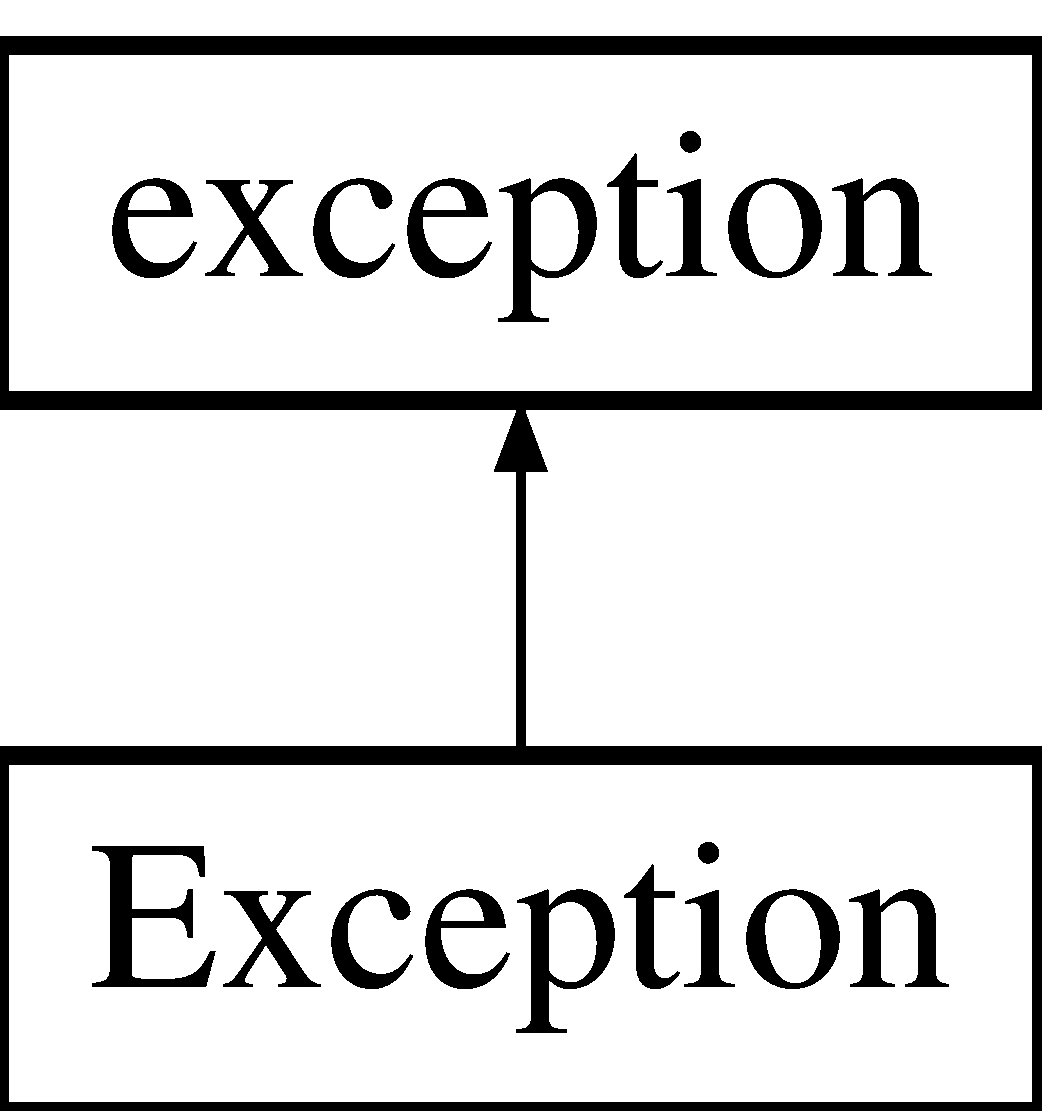
\includegraphics[height=2.000000cm]{d4/d67/classException}
\end{center}
\end{figure}
\subsection*{Public Member Functions}
\begin{DoxyCompactItemize}
\item 
\hyperlink{classException_a1b78336bb26edf8e784783cc150c5801}{Exception} ()
\item 
\hyperlink{classException_a63246c90246de105568d97b0164954d8}{Exception} (std\-::string)
\item 
std\-::string \hyperlink{classException_ae40b22a7b2471b142d861bc33b51a820}{what} ()
\item 
\hyperlink{classException_a6b214cd8627d0968bdeebc1fbb9556b8}{$\sim$\-Exception} ()  throw ()
\end{DoxyCompactItemize}
\subsection*{Private Attributes}
\begin{DoxyCompactItemize}
\item 
std\-::string \hyperlink{classException_a404e79b557f64d95acfb5dccbb864860}{text\-\_\-}
\end{DoxyCompactItemize}


\subsection{Constructor \& Destructor Documentation}
\hypertarget{classException_a1b78336bb26edf8e784783cc150c5801}{\index{Exception@{Exception}!Exception@{Exception}}
\index{Exception@{Exception}!Exception@{Exception}}
\subsubsection[{Exception}]{\setlength{\rightskip}{0pt plus 5cm}Exception\-::\-Exception (
\begin{DoxyParamCaption}
{}
\end{DoxyParamCaption}
)}}\label{classException_a1b78336bb26edf8e784783cc150c5801}
\hypertarget{classException_a63246c90246de105568d97b0164954d8}{\index{Exception@{Exception}!Exception@{Exception}}
\index{Exception@{Exception}!Exception@{Exception}}
\subsubsection[{Exception}]{\setlength{\rightskip}{0pt plus 5cm}Exception\-::\-Exception (
\begin{DoxyParamCaption}
\item[{std\-::string}]{}
\end{DoxyParamCaption}
)}}\label{classException_a63246c90246de105568d97b0164954d8}
\hypertarget{classException_a6b214cd8627d0968bdeebc1fbb9556b8}{\index{Exception@{Exception}!$\sim$\-Exception@{$\sim$\-Exception}}
\index{$\sim$\-Exception@{$\sim$\-Exception}!Exception@{Exception}}
\subsubsection[{$\sim$\-Exception}]{\setlength{\rightskip}{0pt plus 5cm}Exception\-::$\sim$\-Exception (
\begin{DoxyParamCaption}
{}
\end{DoxyParamCaption}
) throw  ) }}\label{classException_a6b214cd8627d0968bdeebc1fbb9556b8}


\subsection{Member Function Documentation}
\hypertarget{classException_ae40b22a7b2471b142d861bc33b51a820}{\index{Exception@{Exception}!what@{what}}
\index{what@{what}!Exception@{Exception}}
\subsubsection[{what}]{\setlength{\rightskip}{0pt plus 5cm}std\-::string Exception\-::what (
\begin{DoxyParamCaption}
{}
\end{DoxyParamCaption}
)}}\label{classException_ae40b22a7b2471b142d861bc33b51a820}


\subsection{Member Data Documentation}
\hypertarget{classException_a404e79b557f64d95acfb5dccbb864860}{\index{Exception@{Exception}!text\-\_\-@{text\-\_\-}}
\index{text\-\_\-@{text\-\_\-}!Exception@{Exception}}
\subsubsection[{text\-\_\-}]{\setlength{\rightskip}{0pt plus 5cm}std\-::string Exception\-::text\-\_\-\hspace{0.3cm}{\ttfamily [private]}}}\label{classException_a404e79b557f64d95acfb5dccbb864860}


The documentation for this class was generated from the following file\-:\begin{DoxyCompactItemize}
\item 
src/\hyperlink{Exception_8h}{Exception.\-h}\end{DoxyCompactItemize}

\hypertarget{classparser_1_1LRParser}{\section{parser\-:\-:\-L\-R\-Parser \-Class \-Reference}
\label{d6/d50/classparser_1_1LRParser}\index{parser\-::\-L\-R\-Parser@{parser\-::\-L\-R\-Parser}}
}


{\ttfamily \#include $<$\-L\-R\-Parser.\-h$>$}

\-Inheritance diagram for parser\-:\-:\-L\-R\-Parser\-:\begin{figure}[H]
\begin{center}
\leavevmode
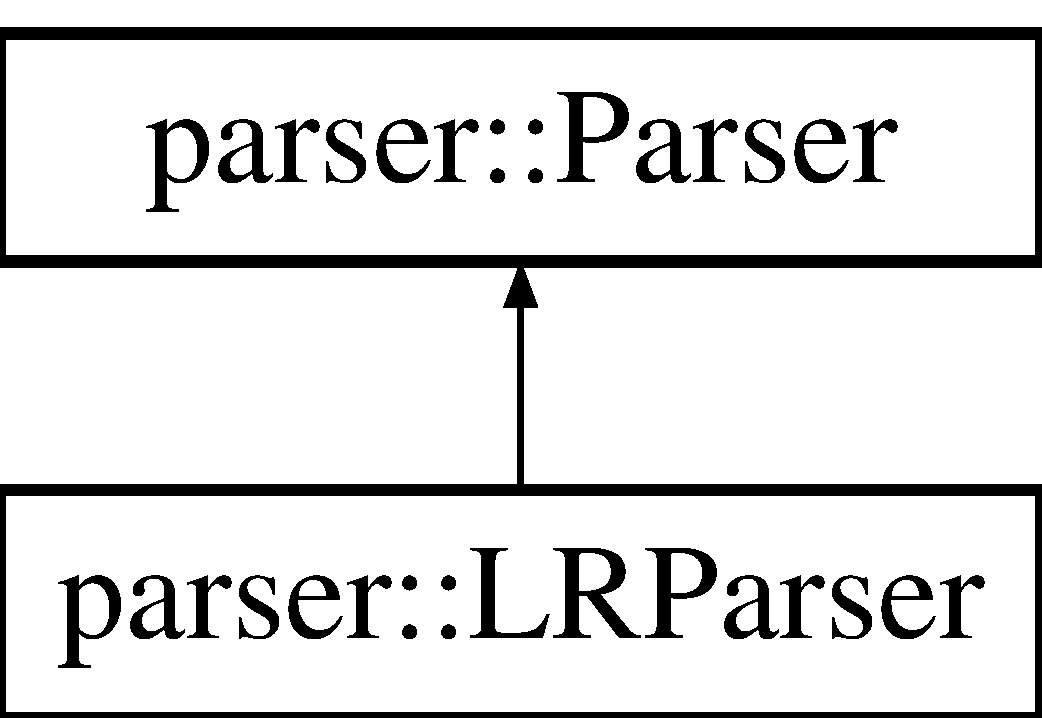
\includegraphics[height=2.000000cm]{d6/d50/classparser_1_1LRParser}
\end{center}
\end{figure}
\subsection*{\-Public \-Member \-Functions}
\begin{DoxyCompactItemize}
\item 
\hyperlink{classparser_1_1LRParser_a47746b2d23e724d5149a51971a92cf7e}{\-L\-R\-Parser} ()
\begin{DoxyCompactList}\small\item\em \-Default constructor for \hyperlink{classparser_1_1LRParser}{\-L\-R\-Parser}. \-This won't be able to do anything as it has no parse table. \end{DoxyCompactList}\item 
\hyperlink{classparser_1_1LRParser_a275c85831be080f6befe55be32e624ca}{\-L\-R\-Parser} (\hyperlink{classGrammar_1_1CFG}{\-Grammar\-::\-C\-F\-G})
\begin{DoxyCompactList}\small\item\em \-The \-C\-F\-G defines the \-C\-F\-L. \-The parse table will be generated from this grammar. \end{DoxyCompactList}\item 
\hyperlink{classparser_1_1LRParser_a14376046af5b5d818b6e46902d765b0d}{\-L\-R\-Parser} (\hyperlink{classparser_1_1ParseTable}{\-Parse\-Table})
\begin{DoxyCompactList}\small\item\em \-The parameter \hyperlink{classparser_1_1ParseTable}{\-Parse\-Table} will be directly used. \end{DoxyCompactList}\item 
bool \hyperlink{classparser_1_1LRParser_ab2152a22b9f4df294863ea2ecb5bea2a}{parse} (std\-::string)
\begin{DoxyCompactList}\small\item\em \-Parses the given input string and returns true if it is valid, false if it is invalid. \end{DoxyCompactList}\item 
std\-::stack$<$ std\-::string $>$ \hyperlink{classparser_1_1LRParser_afb2888c56509ee1b5252e825b48eaf60}{get\-Stack} ()
\item 
unsigned int \hyperlink{classparser_1_1LRParser_a71371a8a7881011135735d46f66aad13}{get\-Counter} ()
\item 
virtual \hyperlink{classparser_1_1LRParser_a786f8c43582c5f620fb6d9f077be2af5}{$\sim$\-L\-R\-Parser} ()
\end{DoxyCompactItemize}
\subsection*{\-Protected \-Member \-Functions}
\begin{DoxyCompactItemize}
\item 
std\-::pair$<$ \hyperlink{namespaceparser_a7a838229f5b5b20f185dfad9d362dbed}{\-E\-Action}, std\-::string $>$ \hyperlink{classparser_1_1LRParser_ac9e3368e99728ed520337590ca04871b}{process\-Symbol} ()
\begin{DoxyCompactList}\small\item\em \-Counter used to track at what character of our input we're at. \end{DoxyCompactList}\item 
bool \hyperlink{classparser_1_1LRParser_a4999e6f888dd298d99ad945f95f1b9b6}{perform\-Action} (std\-::pair$<$ \hyperlink{namespaceparser_a7a838229f5b5b20f185dfad9d362dbed}{\-E\-Action}, std\-::string $>$)
\begin{DoxyCompactList}\small\item\em \-Performs action. \-If this evaluates to true the function it means that input\-\_\- was valid. \end{DoxyCompactList}\item 
bool \hyperlink{classparser_1_1LRParser_a1752e1adccefa9865a327eb4b0554103}{handle\-Reduction} (std\-::string)
\begin{DoxyCompactList}\small\item\em \-Handles the reduction action. \end{DoxyCompactList}\end{DoxyCompactItemize}
\subsection*{\-Protected \-Attributes}
\begin{DoxyCompactItemize}
\item 
\hyperlink{classparser_1_1ParseTable}{\-Parse\-Table} \hyperlink{classparser_1_1LRParser_a2d47acce2ed64522ddd4011295412e72}{p\-\_\-table\-\_\-}
\item 
std\-::stack$<$ std\-::string $>$ \hyperlink{classparser_1_1LRParser_a6e3689c510e91dbc51a2bee92bf760da}{stack\-\_\-}
\item 
std\-::string \hyperlink{classparser_1_1LRParser_a7d693202c661afc170b2c5cc11667323}{input\-\_\-}
\item 
unsigned int \hyperlink{classparser_1_1LRParser_accf01c8956117b364f88fba4cb17b15c}{counter\-\_\-}
\end{DoxyCompactItemize}
\subsection*{\-Friends}
\begin{DoxyCompactItemize}
\item 
std\-::ostream \& \hyperlink{classparser_1_1LRParser_a9f53bcd94244f30103c9756aabf51d38}{operator$<$$<$} (std\-::ostream \&, \hyperlink{classparser_1_1LRParser}{\-L\-R\-Parser} \&)
\begin{DoxyCompactList}\small\item\em \-Overloaded output operator\-: shows the stack contents;. \end{DoxyCompactList}\end{DoxyCompactItemize}


\subsection{\-Constructor \& \-Destructor \-Documentation}
\hypertarget{classparser_1_1LRParser_a47746b2d23e724d5149a51971a92cf7e}{\index{parser\-::\-L\-R\-Parser@{parser\-::\-L\-R\-Parser}!\-L\-R\-Parser@{\-L\-R\-Parser}}
\index{\-L\-R\-Parser@{\-L\-R\-Parser}!parser::LRParser@{parser\-::\-L\-R\-Parser}}
\subsubsection[{\-L\-R\-Parser}]{\setlength{\rightskip}{0pt plus 5cm}{\bf parser\-::\-L\-R\-Parser\-::\-L\-R\-Parser} (
\begin{DoxyParamCaption}
{}
\end{DoxyParamCaption}
)}}\label{d6/d50/classparser_1_1LRParser_a47746b2d23e724d5149a51971a92cf7e}


\-Default constructor for \hyperlink{classparser_1_1LRParser}{\-L\-R\-Parser}. \-This won't be able to do anything as it has no parse table. 

\hypertarget{classparser_1_1LRParser_a275c85831be080f6befe55be32e624ca}{\index{parser\-::\-L\-R\-Parser@{parser\-::\-L\-R\-Parser}!\-L\-R\-Parser@{\-L\-R\-Parser}}
\index{\-L\-R\-Parser@{\-L\-R\-Parser}!parser::LRParser@{parser\-::\-L\-R\-Parser}}
\subsubsection[{\-L\-R\-Parser}]{\setlength{\rightskip}{0pt plus 5cm}{\bf parser\-::\-L\-R\-Parser\-::\-L\-R\-Parser} (
\begin{DoxyParamCaption}
\item[{{\bf \-Grammar\-::\-C\-F\-G}}]{}
\end{DoxyParamCaption}
)}}\label{d6/d50/classparser_1_1LRParser_a275c85831be080f6befe55be32e624ca}


\-The \-C\-F\-G defines the \-C\-F\-L. \-The parse table will be generated from this grammar. 


\begin{DoxyParams}{\-Parameters}
{\em grammar} & grammar for our \hyperlink{classparser_1_1LRParser}{\-L\-R\-Parser}. \\
\hline
\end{DoxyParams}
\hypertarget{classparser_1_1LRParser_a14376046af5b5d818b6e46902d765b0d}{\index{parser\-::\-L\-R\-Parser@{parser\-::\-L\-R\-Parser}!\-L\-R\-Parser@{\-L\-R\-Parser}}
\index{\-L\-R\-Parser@{\-L\-R\-Parser}!parser::LRParser@{parser\-::\-L\-R\-Parser}}
\subsubsection[{\-L\-R\-Parser}]{\setlength{\rightskip}{0pt plus 5cm}{\bf parser\-::\-L\-R\-Parser\-::\-L\-R\-Parser} (
\begin{DoxyParamCaption}
\item[{{\bf \-Parse\-Table}}]{}
\end{DoxyParamCaption}
)}}\label{d6/d50/classparser_1_1LRParser_a14376046af5b5d818b6e46902d765b0d}


\-The parameter \hyperlink{classparser_1_1ParseTable}{\-Parse\-Table} will be directly used. 


\begin{DoxyParams}{\-Parameters}
{\em pt} & \hyperlink{classparser_1_1ParseTable}{\-Parse\-Table} for our \hyperlink{classparser_1_1LRParser}{\-L\-R\-Parser}. \\
\hline
\end{DoxyParams}
\hypertarget{classparser_1_1LRParser_a786f8c43582c5f620fb6d9f077be2af5}{\index{parser\-::\-L\-R\-Parser@{parser\-::\-L\-R\-Parser}!$\sim$\-L\-R\-Parser@{$\sim$\-L\-R\-Parser}}
\index{$\sim$\-L\-R\-Parser@{$\sim$\-L\-R\-Parser}!parser::LRParser@{parser\-::\-L\-R\-Parser}}
\subsubsection[{$\sim$\-L\-R\-Parser}]{\setlength{\rightskip}{0pt plus 5cm}virtual {\bf parser\-::\-L\-R\-Parser\-::$\sim$\-L\-R\-Parser} (
\begin{DoxyParamCaption}
{}
\end{DoxyParamCaption}
)\hspace{0.3cm}{\ttfamily  \mbox{[}virtual\mbox{]}}}}\label{d6/d50/classparser_1_1LRParser_a786f8c43582c5f620fb6d9f077be2af5}


\subsection{\-Member \-Function \-Documentation}
\hypertarget{classparser_1_1LRParser_a71371a8a7881011135735d46f66aad13}{\index{parser\-::\-L\-R\-Parser@{parser\-::\-L\-R\-Parser}!get\-Counter@{get\-Counter}}
\index{get\-Counter@{get\-Counter}!parser::LRParser@{parser\-::\-L\-R\-Parser}}
\subsubsection[{get\-Counter}]{\setlength{\rightskip}{0pt plus 5cm}unsigned int {\bf parser\-::\-L\-R\-Parser\-::get\-Counter} (
\begin{DoxyParamCaption}
{}
\end{DoxyParamCaption}
)}}\label{d6/d50/classparser_1_1LRParser_a71371a8a7881011135735d46f66aad13}
\hypertarget{classparser_1_1LRParser_afb2888c56509ee1b5252e825b48eaf60}{\index{parser\-::\-L\-R\-Parser@{parser\-::\-L\-R\-Parser}!get\-Stack@{get\-Stack}}
\index{get\-Stack@{get\-Stack}!parser::LRParser@{parser\-::\-L\-R\-Parser}}
\subsubsection[{get\-Stack}]{\setlength{\rightskip}{0pt plus 5cm}std\-::stack$<$std\-::string$>$ {\bf parser\-::\-L\-R\-Parser\-::get\-Stack} (
\begin{DoxyParamCaption}
{}
\end{DoxyParamCaption}
)}}\label{d6/d50/classparser_1_1LRParser_afb2888c56509ee1b5252e825b48eaf60}
\hypertarget{classparser_1_1LRParser_a1752e1adccefa9865a327eb4b0554103}{\index{parser\-::\-L\-R\-Parser@{parser\-::\-L\-R\-Parser}!handle\-Reduction@{handle\-Reduction}}
\index{handle\-Reduction@{handle\-Reduction}!parser::LRParser@{parser\-::\-L\-R\-Parser}}
\subsubsection[{handle\-Reduction}]{\setlength{\rightskip}{0pt plus 5cm}bool {\bf parser\-::\-L\-R\-Parser\-::handle\-Reduction} (
\begin{DoxyParamCaption}
\item[{std\-::string}]{}
\end{DoxyParamCaption}
)\hspace{0.3cm}{\ttfamily  \mbox{[}protected\mbox{]}}}}\label{d6/d50/classparser_1_1LRParser_a1752e1adccefa9865a327eb4b0554103}


\-Handles the reduction action. 


\begin{DoxyParams}{\-Parameters}
{\em input} & is a rule that will be applied from body to head. \\
\hline
\end{DoxyParams}
\hypertarget{classparser_1_1LRParser_ab2152a22b9f4df294863ea2ecb5bea2a}{\index{parser\-::\-L\-R\-Parser@{parser\-::\-L\-R\-Parser}!parse@{parse}}
\index{parse@{parse}!parser::LRParser@{parser\-::\-L\-R\-Parser}}
\subsubsection[{parse}]{\setlength{\rightskip}{0pt plus 5cm}bool {\bf parser\-::\-L\-R\-Parser\-::parse} (
\begin{DoxyParamCaption}
\item[{std\-::string}]{}
\end{DoxyParamCaption}
)}}\label{d6/d50/classparser_1_1LRParser_ab2152a22b9f4df294863ea2ecb5bea2a}


\-Parses the given input string and returns true if it is valid, false if it is invalid. 


\begin{DoxyParams}{\-Parameters}
{\em input} & input string that will be tested. \\
\hline
\end{DoxyParams}
\hypertarget{classparser_1_1LRParser_a4999e6f888dd298d99ad945f95f1b9b6}{\index{parser\-::\-L\-R\-Parser@{parser\-::\-L\-R\-Parser}!perform\-Action@{perform\-Action}}
\index{perform\-Action@{perform\-Action}!parser::LRParser@{parser\-::\-L\-R\-Parser}}
\subsubsection[{perform\-Action}]{\setlength{\rightskip}{0pt plus 5cm}bool {\bf parser\-::\-L\-R\-Parser\-::perform\-Action} (
\begin{DoxyParamCaption}
\item[{std\-::pair$<$ {\bf \-E\-Action}, std\-::string $>$}]{}
\end{DoxyParamCaption}
)\hspace{0.3cm}{\ttfamily  \mbox{[}protected\mbox{]}}}}\label{d6/d50/classparser_1_1LRParser_a4999e6f888dd298d99ad945f95f1b9b6}


\-Performs action. \-If this evaluates to true the function it means that input\-\_\- was valid. 


\begin{DoxyParams}{\-Parameters}
{\em action} & which will be executed. \\
\hline
\end{DoxyParams}
\hypertarget{classparser_1_1LRParser_ac9e3368e99728ed520337590ca04871b}{\index{parser\-::\-L\-R\-Parser@{parser\-::\-L\-R\-Parser}!process\-Symbol@{process\-Symbol}}
\index{process\-Symbol@{process\-Symbol}!parser::LRParser@{parser\-::\-L\-R\-Parser}}
\subsubsection[{process\-Symbol}]{\setlength{\rightskip}{0pt plus 5cm}std\-::pair$<${\bf \-E\-Action}, std\-::string$>$ {\bf parser\-::\-L\-R\-Parser\-::process\-Symbol} (
\begin{DoxyParamCaption}
{}
\end{DoxyParamCaption}
)\hspace{0.3cm}{\ttfamily  \mbox{[}protected\mbox{]}}}}\label{d6/d50/classparser_1_1LRParser_ac9e3368e99728ed520337590ca04871b}


\-Counter used to track at what character of our input we're at. 

\-Reads a symbol from the input and returns what to do. (from parsetable) \-Also pushes the read symbol on the stack. \begin{DoxyReturn}{\-Returns}
a pair of what to do (\-E\-Action) and possible data needed for the action (string). 
\end{DoxyReturn}


\subsection{\-Friends \-And \-Related \-Function \-Documentation}
\hypertarget{classparser_1_1LRParser_a9f53bcd94244f30103c9756aabf51d38}{\index{parser\-::\-L\-R\-Parser@{parser\-::\-L\-R\-Parser}!operator$<$$<$@{operator$<$$<$}}
\index{operator$<$$<$@{operator$<$$<$}!parser::LRParser@{parser\-::\-L\-R\-Parser}}
\subsubsection[{operator$<$$<$}]{\setlength{\rightskip}{0pt plus 5cm}std\-::ostream\& operator$<$$<$ (
\begin{DoxyParamCaption}
\item[{std\-::ostream \&}]{, }
\item[{{\bf \-L\-R\-Parser} \&}]{}
\end{DoxyParamCaption}
)\hspace{0.3cm}{\ttfamily  \mbox{[}friend\mbox{]}}}}\label{d6/d50/classparser_1_1LRParser_a9f53bcd94244f30103c9756aabf51d38}


\-Overloaded output operator\-: shows the stack contents;. 



\subsection{\-Member \-Data \-Documentation}
\hypertarget{classparser_1_1LRParser_accf01c8956117b364f88fba4cb17b15c}{\index{parser\-::\-L\-R\-Parser@{parser\-::\-L\-R\-Parser}!counter\-\_\-@{counter\-\_\-}}
\index{counter\-\_\-@{counter\-\_\-}!parser::LRParser@{parser\-::\-L\-R\-Parser}}
\subsubsection[{counter\-\_\-}]{\setlength{\rightskip}{0pt plus 5cm}unsigned int {\bf parser\-::\-L\-R\-Parser\-::counter\-\_\-}\hspace{0.3cm}{\ttfamily  \mbox{[}protected\mbox{]}}}}\label{d6/d50/classparser_1_1LRParser_accf01c8956117b364f88fba4cb17b15c}
\hypertarget{classparser_1_1LRParser_a7d693202c661afc170b2c5cc11667323}{\index{parser\-::\-L\-R\-Parser@{parser\-::\-L\-R\-Parser}!input\-\_\-@{input\-\_\-}}
\index{input\-\_\-@{input\-\_\-}!parser::LRParser@{parser\-::\-L\-R\-Parser}}
\subsubsection[{input\-\_\-}]{\setlength{\rightskip}{0pt plus 5cm}std\-::string {\bf parser\-::\-L\-R\-Parser\-::input\-\_\-}\hspace{0.3cm}{\ttfamily  \mbox{[}protected\mbox{]}}}}\label{d6/d50/classparser_1_1LRParser_a7d693202c661afc170b2c5cc11667323}
\hypertarget{classparser_1_1LRParser_a2d47acce2ed64522ddd4011295412e72}{\index{parser\-::\-L\-R\-Parser@{parser\-::\-L\-R\-Parser}!p\-\_\-table\-\_\-@{p\-\_\-table\-\_\-}}
\index{p\-\_\-table\-\_\-@{p\-\_\-table\-\_\-}!parser::LRParser@{parser\-::\-L\-R\-Parser}}
\subsubsection[{p\-\_\-table\-\_\-}]{\setlength{\rightskip}{0pt plus 5cm}{\bf \-Parse\-Table} {\bf parser\-::\-L\-R\-Parser\-::p\-\_\-table\-\_\-}\hspace{0.3cm}{\ttfamily  \mbox{[}protected\mbox{]}}}}\label{d6/d50/classparser_1_1LRParser_a2d47acce2ed64522ddd4011295412e72}
\hypertarget{classparser_1_1LRParser_a6e3689c510e91dbc51a2bee92bf760da}{\index{parser\-::\-L\-R\-Parser@{parser\-::\-L\-R\-Parser}!stack\-\_\-@{stack\-\_\-}}
\index{stack\-\_\-@{stack\-\_\-}!parser::LRParser@{parser\-::\-L\-R\-Parser}}
\subsubsection[{stack\-\_\-}]{\setlength{\rightskip}{0pt plus 5cm}std\-::stack$<$std\-::string$>$ {\bf parser\-::\-L\-R\-Parser\-::stack\-\_\-}\hspace{0.3cm}{\ttfamily  \mbox{[}protected\mbox{]}}}}\label{d6/d50/classparser_1_1LRParser_a6e3689c510e91dbc51a2bee92bf760da}


\-The documentation for this class was generated from the following file\-:\begin{DoxyCompactItemize}
\item 
src/\hyperlink{LRParser_8h}{\-L\-R\-Parser.\-h}\end{DoxyCompactItemize}

\hypertarget{classparser_1_1Parser}{\section{parser\-:\-:\-Parser \-Class \-Reference}
\label{da/d20/classparser_1_1Parser}\index{parser\-::\-Parser@{parser\-::\-Parser}}
}


{\ttfamily \#include $<$\-Parser.\-h$>$}

\-Inheritance diagram for parser\-:\-:\-Parser\-:\begin{figure}[H]
\begin{center}
\leavevmode
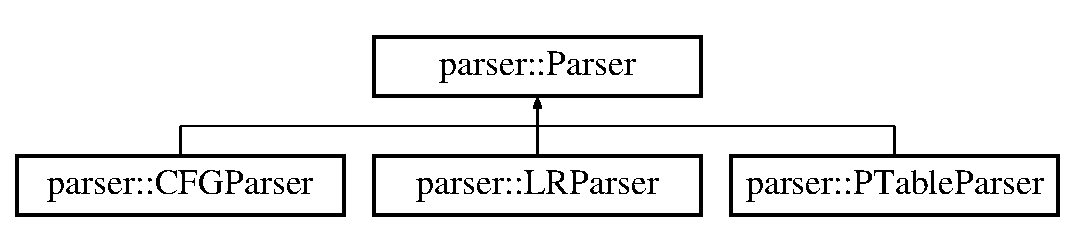
\includegraphics[height=2.000000cm]{da/d20/classparser_1_1Parser}
\end{center}
\end{figure}
\subsection*{\-Public \-Member \-Functions}
\begin{DoxyCompactItemize}
\item 
\hyperlink{classparser_1_1Parser_a359427f631eea550f943676163e9eb68}{\-Parser} ()
\item 
virtual \hyperlink{classparser_1_1Parser_a50675ceb68a2be8df41784b094ef058f}{$\sim$\-Parser} ()
\end{DoxyCompactItemize}


\subsection{\-Constructor \& \-Destructor \-Documentation}
\hypertarget{classparser_1_1Parser_a359427f631eea550f943676163e9eb68}{\index{parser\-::\-Parser@{parser\-::\-Parser}!\-Parser@{\-Parser}}
\index{\-Parser@{\-Parser}!parser::Parser@{parser\-::\-Parser}}
\subsubsection[{\-Parser}]{\setlength{\rightskip}{0pt plus 5cm}{\bf parser\-::\-Parser\-::\-Parser} (
\begin{DoxyParamCaption}
{}
\end{DoxyParamCaption}
)}}\label{da/d20/classparser_1_1Parser_a359427f631eea550f943676163e9eb68}
\hypertarget{classparser_1_1Parser_a50675ceb68a2be8df41784b094ef058f}{\index{parser\-::\-Parser@{parser\-::\-Parser}!$\sim$\-Parser@{$\sim$\-Parser}}
\index{$\sim$\-Parser@{$\sim$\-Parser}!parser::Parser@{parser\-::\-Parser}}
\subsubsection[{$\sim$\-Parser}]{\setlength{\rightskip}{0pt plus 5cm}virtual {\bf parser\-::\-Parser\-::$\sim$\-Parser} (
\begin{DoxyParamCaption}
{}
\end{DoxyParamCaption}
)\hspace{0.3cm}{\ttfamily  \mbox{[}virtual\mbox{]}}}}\label{da/d20/classparser_1_1Parser_a50675ceb68a2be8df41784b094ef058f}


\-The documentation for this class was generated from the following file\-:\begin{DoxyCompactItemize}
\item 
src/\hyperlink{Parser_8h}{\-Parser.\-h}\end{DoxyCompactItemize}

\hypertarget{classparser_1_1ParseTable}{\section{parser\-:\-:\-Parse\-Table \-Class \-Reference}
\label{d6/d64/classparser_1_1ParseTable}\index{parser\-::\-Parse\-Table@{parser\-::\-Parse\-Table}}
}


{\ttfamily \#include $<$\-Parse\-Table.\-h$>$}

\subsection*{\-Public \-Member \-Functions}
\begin{DoxyCompactItemize}
\item 
\hyperlink{classparser_1_1ParseTable_a00ed64dc142ed6ff9418bec52ae3db04}{\-Parse\-Table} ()
\begin{DoxyCompactList}\small\item\em \-Default constructor. \-Our \hyperlink{classparser_1_1ParseTable}{\-Parse\-Table} will be empty as it has no \-C\-F\-G. \end{DoxyCompactList}\item 
\hyperlink{classparser_1_1ParseTable_a4cab1aeb721c0375dbf426ee2200dee4}{\-Parse\-Table} (\hyperlink{classGrammar_1_1CFG}{\-Grammar\-::\-C\-F\-G}, std\-::string)
\begin{DoxyCompactList}\small\item\em \-Our \hyperlink{classparser_1_1ParseTable}{\-Parse\-Table} will be constructed using the \-C\-F\-G provided as parameter. \end{DoxyCompactList}\item 
std\-::pair$<$ \hyperlink{namespaceparser_a7a838229f5b5b20f185dfad9d362dbed}{\-E\-Action}, std\-::string $>$ \hyperlink{classparser_1_1ParseTable_a26500ede234e76d28fcc6bef9198b71a}{operator()} (int, std\-::string) const 
\begin{DoxyCompactList}\small\item\em \-Returns the contents of the parse table (and what action should happen) depending on the input. \end{DoxyCompactList}\item 
virtual \hyperlink{classparser_1_1ParseTable_a9879c15d87bea61cdfbf3e58151e57d3}{$\sim$\-Parse\-Table} ()
\end{DoxyCompactItemize}
\subsection*{\-Private \-Member \-Functions}
\begin{DoxyCompactItemize}
\item 
std\-::pair$<$ \hyperlink{namespaceparser_a7a838229f5b5b20f185dfad9d362dbed}{\-E\-Action}, std\-::string $>$ \hyperlink{classparser_1_1ParseTable_aa82b236a735f2f0b9aff02273c9c96a8}{extract\-Info} (std\-::string) const 
\begin{DoxyCompactList}\small\item\em \-Extracts info from input. \end{DoxyCompactList}\end{DoxyCompactItemize}
\subsection*{\-Private \-Attributes}
\begin{DoxyCompactItemize}
\item 
std\-::vector$<$ std\-::vector\*
$<$ std\-::string $>$ $>$ \hyperlink{classparser_1_1ParseTable_a3dd2e7557544f4b8f55b2817b82992c4}{table}
\begin{DoxyCompactList}\small\item\em \-The actual parse table. \end{DoxyCompactList}\item 
std\-::map$<$ std\-::string, int $>$ \hyperlink{classparser_1_1ParseTable_a5a5d69d3c668e67bf8805165797fca65}{lookup}
\begin{DoxyCompactList}\small\item\em \-Maps column index and input string. \-This is a private method used to quickly find what column index you have to look in. \end{DoxyCompactList}\end{DoxyCompactItemize}


\subsection{\-Constructor \& \-Destructor \-Documentation}
\hypertarget{classparser_1_1ParseTable_a00ed64dc142ed6ff9418bec52ae3db04}{\index{parser\-::\-Parse\-Table@{parser\-::\-Parse\-Table}!\-Parse\-Table@{\-Parse\-Table}}
\index{\-Parse\-Table@{\-Parse\-Table}!parser::ParseTable@{parser\-::\-Parse\-Table}}
\subsubsection[{\-Parse\-Table}]{\setlength{\rightskip}{0pt plus 5cm}{\bf parser\-::\-Parse\-Table\-::\-Parse\-Table} (
\begin{DoxyParamCaption}
{}
\end{DoxyParamCaption}
)}}\label{d6/d64/classparser_1_1ParseTable_a00ed64dc142ed6ff9418bec52ae3db04}


\-Default constructor. \-Our \hyperlink{classparser_1_1ParseTable}{\-Parse\-Table} will be empty as it has no \-C\-F\-G. 

\hypertarget{classparser_1_1ParseTable_a4cab1aeb721c0375dbf426ee2200dee4}{\index{parser\-::\-Parse\-Table@{parser\-::\-Parse\-Table}!\-Parse\-Table@{\-Parse\-Table}}
\index{\-Parse\-Table@{\-Parse\-Table}!parser::ParseTable@{parser\-::\-Parse\-Table}}
\subsubsection[{\-Parse\-Table}]{\setlength{\rightskip}{0pt plus 5cm}{\bf parser\-::\-Parse\-Table\-::\-Parse\-Table} (
\begin{DoxyParamCaption}
\item[{{\bf \-Grammar\-::\-C\-F\-G}}]{, }
\item[{std\-::string}]{}
\end{DoxyParamCaption}
)}}\label{d6/d64/classparser_1_1ParseTable_a4cab1aeb721c0375dbf426ee2200dee4}


\-Our \hyperlink{classparser_1_1ParseTable}{\-Parse\-Table} will be constructed using the \-C\-F\-G provided as parameter. 


\begin{DoxyParams}{\-Parameters}
{\em grammar} & \-The grammar which the \hyperlink{classparser_1_1ParseTable}{\-Parse\-Table} will be based on. \\
\hline
{\em ptable\-X\-M\-L} & \-The filename where our parsetable info can be found. \\
\hline
\end{DoxyParams}
\hypertarget{classparser_1_1ParseTable_a9879c15d87bea61cdfbf3e58151e57d3}{\index{parser\-::\-Parse\-Table@{parser\-::\-Parse\-Table}!$\sim$\-Parse\-Table@{$\sim$\-Parse\-Table}}
\index{$\sim$\-Parse\-Table@{$\sim$\-Parse\-Table}!parser::ParseTable@{parser\-::\-Parse\-Table}}
\subsubsection[{$\sim$\-Parse\-Table}]{\setlength{\rightskip}{0pt plus 5cm}virtual {\bf parser\-::\-Parse\-Table\-::$\sim$\-Parse\-Table} (
\begin{DoxyParamCaption}
{}
\end{DoxyParamCaption}
)\hspace{0.3cm}{\ttfamily  \mbox{[}virtual\mbox{]}}}}\label{d6/d64/classparser_1_1ParseTable_a9879c15d87bea61cdfbf3e58151e57d3}


\subsection{\-Member \-Function \-Documentation}
\hypertarget{classparser_1_1ParseTable_aa82b236a735f2f0b9aff02273c9c96a8}{\index{parser\-::\-Parse\-Table@{parser\-::\-Parse\-Table}!extract\-Info@{extract\-Info}}
\index{extract\-Info@{extract\-Info}!parser::ParseTable@{parser\-::\-Parse\-Table}}
\subsubsection[{extract\-Info}]{\setlength{\rightskip}{0pt plus 5cm}std\-::pair$<${\bf \-E\-Action}, std\-::string$>$ {\bf parser\-::\-Parse\-Table\-::extract\-Info} (
\begin{DoxyParamCaption}
\item[{std\-::string}]{}
\end{DoxyParamCaption}
) const\hspace{0.3cm}{\ttfamily  \mbox{[}private\mbox{]}}}}\label{d6/d64/classparser_1_1ParseTable_aa82b236a735f2f0b9aff02273c9c96a8}


\-Extracts info from input. 


\begin{DoxyParams}{\-Parameters}
{\em entry} & \-A table entry \\
\hline
\end{DoxyParams}
\begin{DoxyReturn}{\-Returns}
\-A pair of what needs to be done (\-E\-Action) and a string with info needed to perform the action. 
\end{DoxyReturn}
\hypertarget{classparser_1_1ParseTable_a26500ede234e76d28fcc6bef9198b71a}{\index{parser\-::\-Parse\-Table@{parser\-::\-Parse\-Table}!operator()@{operator()}}
\index{operator()@{operator()}!parser::ParseTable@{parser\-::\-Parse\-Table}}
\subsubsection[{operator()}]{\setlength{\rightskip}{0pt plus 5cm}std\-::pair$<${\bf \-E\-Action}, std\-::string$>$ parser\-::\-Parse\-Table\-::operator() (
\begin{DoxyParamCaption}
\item[{int}]{, }
\item[{std\-::string}]{}
\end{DoxyParamCaption}
) const}}\label{d6/d64/classparser_1_1ParseTable_a26500ede234e76d28fcc6bef9198b71a}


\-Returns the contents of the parse table (and what action should happen) depending on the input. 


\begin{DoxyParams}{\-Parameters}
{\em token} & \hyperlink{classparser_1_1ParseTable}{\-Parse\-Table} row \\
\hline
{\em symbol} & \hyperlink{classparser_1_1ParseTable}{\-Parse\-Table} column \\
\hline
\end{DoxyParams}
\begin{DoxyReturn}{\-Returns}
\-Pair of an action (\-E\-Action) and possible information needed to complete the action (string) 
\end{DoxyReturn}


\subsection{\-Member \-Data \-Documentation}
\hypertarget{classparser_1_1ParseTable_a5a5d69d3c668e67bf8805165797fca65}{\index{parser\-::\-Parse\-Table@{parser\-::\-Parse\-Table}!lookup@{lookup}}
\index{lookup@{lookup}!parser::ParseTable@{parser\-::\-Parse\-Table}}
\subsubsection[{lookup}]{\setlength{\rightskip}{0pt plus 5cm}std\-::map$<$std\-::string, int$>$ {\bf parser\-::\-Parse\-Table\-::lookup}\hspace{0.3cm}{\ttfamily  \mbox{[}private\mbox{]}}}}\label{d6/d64/classparser_1_1ParseTable_a5a5d69d3c668e67bf8805165797fca65}


\-Maps column index and input string. \-This is a private method used to quickly find what column index you have to look in. 

\hypertarget{classparser_1_1ParseTable_a3dd2e7557544f4b8f55b2817b82992c4}{\index{parser\-::\-Parse\-Table@{parser\-::\-Parse\-Table}!table@{table}}
\index{table@{table}!parser::ParseTable@{parser\-::\-Parse\-Table}}
\subsubsection[{table}]{\setlength{\rightskip}{0pt plus 5cm}std\-::vector$<$std\-::vector$<$std\-::string$>$ $>$ {\bf parser\-::\-Parse\-Table\-::table}\hspace{0.3cm}{\ttfamily  \mbox{[}private\mbox{]}}}}\label{d6/d64/classparser_1_1ParseTable_a3dd2e7557544f4b8f55b2817b82992c4}


\-The actual parse table. 



\-The documentation for this class was generated from the following file\-:\begin{DoxyCompactItemize}
\item 
src/\hyperlink{ParseTable_8h}{\-Parse\-Table.\-h}\end{DoxyCompactItemize}

\hypertarget{classPDA_1_1PDA}{\section{P\-D\-A\-:\-:P\-D\-A Class Reference}
\label{classPDA_1_1PDA}\index{P\-D\-A\-::\-P\-D\-A@{P\-D\-A\-::\-P\-D\-A}}
}


{\ttfamily \#include $<$P\-D\-A.\-h$>$}

\subsection*{Public Member Functions}
\begin{DoxyCompactItemize}
\item 
\hyperlink{classPDA_1_1PDA_a7785c447944c57243e2b1ea76903e3f6}{P\-D\-A} ()
\begin{DoxyCompactList}\small\item\em A standard constructor. \end{DoxyCompactList}\item 
\hyperlink{classPDA_1_1PDA_a457ac4b1de0a21642e946847b85fcc2b}{P\-D\-A} (\hyperlink{classCFG}{C\-F\-G} $\ast$grammar)
\begin{DoxyCompactList}\small\item\em A specified contstructor. \end{DoxyCompactList}\item 
virtual \hyperlink{classPDA_1_1PDA_a9cd56fae8de9f1cc8a6b3da52d1b525f}{$\sim$\-P\-D\-A} ()
\begin{DoxyCompactList}\small\item\em A standard destructor. \end{DoxyCompactList}\item 
void \hyperlink{classPDA_1_1PDA_adeb9e042e871b40ad01630d4da2e7a6a}{to\-Empty\-Stack\-Acceptance} ()
\begin{DoxyCompactList}\small\item\em A function changing the \hyperlink{classPDA_1_1PDA}{P\-D\-A} to accept by empty stack. \end{DoxyCompactList}\item 
void \hyperlink{classPDA_1_1PDA_a6c6b86cde5edba8125fcf633d0a9a916}{to\-Final\-State\-Acceptance} ()
\begin{DoxyCompactList}\small\item\em A function changing the \hyperlink{classPDA_1_1PDA}{P\-D\-A} to accept by final state. \end{DoxyCompactList}\item 
void \hyperlink{classPDA_1_1PDA_a741e99b5d9e53e32d6808bf83dde96b2}{to\-La\-Te\-X} (std\-::string filename)
\begin{DoxyCompactList}\small\item\em A function making a file to print the \hyperlink{classPDA_1_1PDA}{P\-D\-A} in La\-Te\-X. \end{DoxyCompactList}\item 
void \hyperlink{classPDA_1_1PDA_a04c7164ddd8488e074741259cb9a8db4}{print\-\_\-status} ()
\begin{DoxyCompactList}\small\item\em A function to print the complete current status of the \hyperlink{classPDA_1_1PDA}{P\-D\-A}. \end{DoxyCompactList}\end{DoxyCompactItemize}
\subsection*{Private Member Functions}
\begin{DoxyCompactItemize}
\item 
std\-::string \hyperlink{classPDA_1_1PDA_af707f305d9b16dbc3dcb686a3f63fca4}{check\-State\-Names} (std\-::string prefix)
\begin{DoxyCompactList}\small\item\em A pair containing a pointer to the current state we are in and its corresponding stack. \end{DoxyCompactList}\item 
bool \hyperlink{classPDA_1_1PDA_aa245040d766419cc4e9ddcd825ab6ca5}{is\-Accept\-State} (std\-::string name)
\begin{DoxyCompactList}\small\item\em Returns whether a certain state is an accept state. \end{DoxyCompactList}\item 
bool \hyperlink{classPDA_1_1PDA_a37329b27d0ac02e944d1160a4462fbce}{is\-Start\-State} (std\-::string name)
\begin{DoxyCompactList}\small\item\em Returns whether a certain state is a start state. \end{DoxyCompactList}\end{DoxyCompactItemize}
\subsection*{Private Attributes}
\begin{DoxyCompactItemize}
\item 
\hyperlink{classCFG}{C\-F\-G} $\ast$ \hyperlink{classPDA_1_1PDA_aef026ff20ec36b368db8cf05dc7d6ef7}{cfg}
\item 
\hyperlink{namespacePDA_a2f2b17cdf30facf6f0fe593ab209acf8}{P\-D\-A\-Type} \hyperlink{classPDA_1_1PDA_a15524b46d2be399f384b0f236ccb38f4}{type}
\begin{DoxyCompactList}\small\item\em A pointer to the \hyperlink{classCFG}{C\-F\-G} equivalent with this \hyperlink{classPDA_1_1PDA}{P\-D\-A}. \end{DoxyCompactList}\item 
std\-::vector$<$ \hyperlink{classPDA_1_1State}{State} $>$ \hyperlink{classPDA_1_1PDA_a38d40f2c938f18d396ea2b13ca361271}{states}
\begin{DoxyCompactList}\small\item\em The type of the \hyperlink{classPDA_1_1PDA}{P\-D\-A} (accept\-By\-Final\-State or accept\-By\-Empty\-Stack). \end{DoxyCompactList}\item 
std\-::vector$<$ char $>$ \hyperlink{classPDA_1_1PDA_a54db260eece0bfe0d5aad0ef13f18a02}{input\-\_\-alphabet}
\begin{DoxyCompactList}\small\item\em A vector containing all the states of the \hyperlink{classPDA_1_1PDA}{P\-D\-A}. \end{DoxyCompactList}\item 
std\-::vector$<$ std\-::string $>$ \hyperlink{classPDA_1_1PDA_a90a4f96e28003d5bfa4d67b4c7a191b5}{stack\-\_\-alphabet}
\begin{DoxyCompactList}\small\item\em A vector containing all the symbols that can be used as input. \end{DoxyCompactList}\item 
std\-::string \hyperlink{classPDA_1_1PDA_af346efb9a6812d704d69299eef9262e6}{start\-\_\-state}
\begin{DoxyCompactList}\small\item\em A vector containing all the symbols used on the stack. \end{DoxyCompactList}\item 
std\-::string \hyperlink{classPDA_1_1PDA_a253c02338c616cd8e8882f71e2a5666f}{start\-\_\-stack}
\begin{DoxyCompactList}\small\item\em The name of the start state. \end{DoxyCompactList}\item 
std\-::vector$<$ std\-::string $>$ \hyperlink{classPDA_1_1PDA_a7c6d15bda561a77936c986290af7bf66}{accept\-\_\-states}
\begin{DoxyCompactList}\small\item\em The symbol that is initially pushed on the stack. \end{DoxyCompactList}\item 
std\-::vector$<$ std\-::pair$<$ \hyperlink{classPDA_1_1State}{State} \\*
$\ast$, std\-::stack$<$ std\-::string $>$ $>$ $>$ \hyperlink{classPDA_1_1PDA_a71d7a97ddb658ed2c07e30001ff6ba1b}{cur\-\_\-states}
\begin{DoxyCompactList}\small\item\em A vector containing the names of the accept states. \end{DoxyCompactList}\end{DoxyCompactItemize}


\subsection{Constructor \& Destructor Documentation}
\hypertarget{classPDA_1_1PDA_a7785c447944c57243e2b1ea76903e3f6}{\index{P\-D\-A\-::\-P\-D\-A@{P\-D\-A\-::\-P\-D\-A}!P\-D\-A@{P\-D\-A}}
\index{P\-D\-A@{P\-D\-A}!PDA::PDA@{P\-D\-A\-::\-P\-D\-A}}
\subsubsection[{P\-D\-A}]{\setlength{\rightskip}{0pt plus 5cm}P\-D\-A\-::\-P\-D\-A\-::\-P\-D\-A (
\begin{DoxyParamCaption}
{}
\end{DoxyParamCaption}
)}}\label{classPDA_1_1PDA_a7785c447944c57243e2b1ea76903e3f6}


A standard constructor. 

\hypertarget{classPDA_1_1PDA_a457ac4b1de0a21642e946847b85fcc2b}{\index{P\-D\-A\-::\-P\-D\-A@{P\-D\-A\-::\-P\-D\-A}!P\-D\-A@{P\-D\-A}}
\index{P\-D\-A@{P\-D\-A}!PDA::PDA@{P\-D\-A\-::\-P\-D\-A}}
\subsubsection[{P\-D\-A}]{\setlength{\rightskip}{0pt plus 5cm}P\-D\-A\-::\-P\-D\-A\-::\-P\-D\-A (
\begin{DoxyParamCaption}
\item[{{\bf C\-F\-G} $\ast$}]{grammar}
\end{DoxyParamCaption}
)}}\label{classPDA_1_1PDA_a457ac4b1de0a21642e946847b85fcc2b}


A specified contstructor. 


\begin{DoxyParams}{Parameters}
{\em grammar} & A \hyperlink{classCFG}{C\-F\-G} used to create an equivalent \hyperlink{classPDA_1_1PDA}{P\-D\-A}. \\
\hline
\end{DoxyParams}
\hypertarget{classPDA_1_1PDA_a9cd56fae8de9f1cc8a6b3da52d1b525f}{\index{P\-D\-A\-::\-P\-D\-A@{P\-D\-A\-::\-P\-D\-A}!$\sim$\-P\-D\-A@{$\sim$\-P\-D\-A}}
\index{$\sim$\-P\-D\-A@{$\sim$\-P\-D\-A}!PDA::PDA@{P\-D\-A\-::\-P\-D\-A}}
\subsubsection[{$\sim$\-P\-D\-A}]{\setlength{\rightskip}{0pt plus 5cm}virtual P\-D\-A\-::\-P\-D\-A\-::$\sim$\-P\-D\-A (
\begin{DoxyParamCaption}
{}
\end{DoxyParamCaption}
)\hspace{0.3cm}{\ttfamily [virtual]}}}\label{classPDA_1_1PDA_a9cd56fae8de9f1cc8a6b3da52d1b525f}


A standard destructor. 



\subsection{Member Function Documentation}
\hypertarget{classPDA_1_1PDA_af707f305d9b16dbc3dcb686a3f63fca4}{\index{P\-D\-A\-::\-P\-D\-A@{P\-D\-A\-::\-P\-D\-A}!check\-State\-Names@{check\-State\-Names}}
\index{check\-State\-Names@{check\-State\-Names}!PDA::PDA@{P\-D\-A\-::\-P\-D\-A}}
\subsubsection[{check\-State\-Names}]{\setlength{\rightskip}{0pt plus 5cm}std\-::string P\-D\-A\-::\-P\-D\-A\-::check\-State\-Names (
\begin{DoxyParamCaption}
\item[{std\-::string}]{prefix}
\end{DoxyParamCaption}
)\hspace{0.3cm}{\ttfamily [private]}}}\label{classPDA_1_1PDA_af707f305d9b16dbc3dcb686a3f63fca4}


A pair containing a pointer to the current state we are in and its corresponding stack. 

Checks wether a certain name is already used in the \hyperlink{classPDA_1_1PDA}{P\-D\-A}. 
\begin{DoxyParams}{Parameters}
{\em prefix} & Start of the name you want to give the state. \\
\hline
\end{DoxyParams}
\hypertarget{classPDA_1_1PDA_aa245040d766419cc4e9ddcd825ab6ca5}{\index{P\-D\-A\-::\-P\-D\-A@{P\-D\-A\-::\-P\-D\-A}!is\-Accept\-State@{is\-Accept\-State}}
\index{is\-Accept\-State@{is\-Accept\-State}!PDA::PDA@{P\-D\-A\-::\-P\-D\-A}}
\subsubsection[{is\-Accept\-State}]{\setlength{\rightskip}{0pt plus 5cm}bool P\-D\-A\-::\-P\-D\-A\-::is\-Accept\-State (
\begin{DoxyParamCaption}
\item[{std\-::string}]{name}
\end{DoxyParamCaption}
)\hspace{0.3cm}{\ttfamily [private]}}}\label{classPDA_1_1PDA_aa245040d766419cc4e9ddcd825ab6ca5}


Returns whether a certain state is an accept state. 


\begin{DoxyParams}{Parameters}
{\em name} & Name of the state you want to check. \\
\hline
\end{DoxyParams}
\begin{DoxyReturn}{Returns}
A boolean telling whether it is an accept state. 
\end{DoxyReturn}
\hypertarget{classPDA_1_1PDA_a37329b27d0ac02e944d1160a4462fbce}{\index{P\-D\-A\-::\-P\-D\-A@{P\-D\-A\-::\-P\-D\-A}!is\-Start\-State@{is\-Start\-State}}
\index{is\-Start\-State@{is\-Start\-State}!PDA::PDA@{P\-D\-A\-::\-P\-D\-A}}
\subsubsection[{is\-Start\-State}]{\setlength{\rightskip}{0pt plus 5cm}bool P\-D\-A\-::\-P\-D\-A\-::is\-Start\-State (
\begin{DoxyParamCaption}
\item[{std\-::string}]{name}
\end{DoxyParamCaption}
)\hspace{0.3cm}{\ttfamily [private]}}}\label{classPDA_1_1PDA_a37329b27d0ac02e944d1160a4462fbce}


Returns whether a certain state is a start state. 


\begin{DoxyParams}{Parameters}
{\em name} & Name of the state you want to check. \\
\hline
\end{DoxyParams}
\begin{DoxyReturn}{Returns}
A boolean telling whether it is a start state. 
\end{DoxyReturn}
\hypertarget{classPDA_1_1PDA_a04c7164ddd8488e074741259cb9a8db4}{\index{P\-D\-A\-::\-P\-D\-A@{P\-D\-A\-::\-P\-D\-A}!print\-\_\-status@{print\-\_\-status}}
\index{print\-\_\-status@{print\-\_\-status}!PDA::PDA@{P\-D\-A\-::\-P\-D\-A}}
\subsubsection[{print\-\_\-status}]{\setlength{\rightskip}{0pt plus 5cm}void P\-D\-A\-::\-P\-D\-A\-::print\-\_\-status (
\begin{DoxyParamCaption}
{}
\end{DoxyParamCaption}
)}}\label{classPDA_1_1PDA_a04c7164ddd8488e074741259cb9a8db4}


A function to print the complete current status of the \hyperlink{classPDA_1_1PDA}{P\-D\-A}. 

\hypertarget{classPDA_1_1PDA_adeb9e042e871b40ad01630d4da2e7a6a}{\index{P\-D\-A\-::\-P\-D\-A@{P\-D\-A\-::\-P\-D\-A}!to\-Empty\-Stack\-Acceptance@{to\-Empty\-Stack\-Acceptance}}
\index{to\-Empty\-Stack\-Acceptance@{to\-Empty\-Stack\-Acceptance}!PDA::PDA@{P\-D\-A\-::\-P\-D\-A}}
\subsubsection[{to\-Empty\-Stack\-Acceptance}]{\setlength{\rightskip}{0pt plus 5cm}void P\-D\-A\-::\-P\-D\-A\-::to\-Empty\-Stack\-Acceptance (
\begin{DoxyParamCaption}
{}
\end{DoxyParamCaption}
)}}\label{classPDA_1_1PDA_adeb9e042e871b40ad01630d4da2e7a6a}


A function changing the \hyperlink{classPDA_1_1PDA}{P\-D\-A} to accept by empty stack. 

\hypertarget{classPDA_1_1PDA_a6c6b86cde5edba8125fcf633d0a9a916}{\index{P\-D\-A\-::\-P\-D\-A@{P\-D\-A\-::\-P\-D\-A}!to\-Final\-State\-Acceptance@{to\-Final\-State\-Acceptance}}
\index{to\-Final\-State\-Acceptance@{to\-Final\-State\-Acceptance}!PDA::PDA@{P\-D\-A\-::\-P\-D\-A}}
\subsubsection[{to\-Final\-State\-Acceptance}]{\setlength{\rightskip}{0pt plus 5cm}void P\-D\-A\-::\-P\-D\-A\-::to\-Final\-State\-Acceptance (
\begin{DoxyParamCaption}
{}
\end{DoxyParamCaption}
)}}\label{classPDA_1_1PDA_a6c6b86cde5edba8125fcf633d0a9a916}


A function changing the \hyperlink{classPDA_1_1PDA}{P\-D\-A} to accept by final state. 

\hypertarget{classPDA_1_1PDA_a741e99b5d9e53e32d6808bf83dde96b2}{\index{P\-D\-A\-::\-P\-D\-A@{P\-D\-A\-::\-P\-D\-A}!to\-La\-Te\-X@{to\-La\-Te\-X}}
\index{to\-La\-Te\-X@{to\-La\-Te\-X}!PDA::PDA@{P\-D\-A\-::\-P\-D\-A}}
\subsubsection[{to\-La\-Te\-X}]{\setlength{\rightskip}{0pt plus 5cm}void P\-D\-A\-::\-P\-D\-A\-::to\-La\-Te\-X (
\begin{DoxyParamCaption}
\item[{std\-::string}]{filename}
\end{DoxyParamCaption}
)}}\label{classPDA_1_1PDA_a741e99b5d9e53e32d6808bf83dde96b2}


A function making a file to print the \hyperlink{classPDA_1_1PDA}{P\-D\-A} in La\-Te\-X. 


\begin{DoxyParams}{Parameters}
{\em filename} & The name of the file where the .tex file will be created. \\
\hline
\end{DoxyParams}


\subsection{Member Data Documentation}
\hypertarget{classPDA_1_1PDA_a7c6d15bda561a77936c986290af7bf66}{\index{P\-D\-A\-::\-P\-D\-A@{P\-D\-A\-::\-P\-D\-A}!accept\-\_\-states@{accept\-\_\-states}}
\index{accept\-\_\-states@{accept\-\_\-states}!PDA::PDA@{P\-D\-A\-::\-P\-D\-A}}
\subsubsection[{accept\-\_\-states}]{\setlength{\rightskip}{0pt plus 5cm}std\-::vector$<$std\-::string$>$ P\-D\-A\-::\-P\-D\-A\-::accept\-\_\-states\hspace{0.3cm}{\ttfamily [private]}}}\label{classPDA_1_1PDA_a7c6d15bda561a77936c986290af7bf66}


The symbol that is initially pushed on the stack. 

\hypertarget{classPDA_1_1PDA_aef026ff20ec36b368db8cf05dc7d6ef7}{\index{P\-D\-A\-::\-P\-D\-A@{P\-D\-A\-::\-P\-D\-A}!cfg@{cfg}}
\index{cfg@{cfg}!PDA::PDA@{P\-D\-A\-::\-P\-D\-A}}
\subsubsection[{cfg}]{\setlength{\rightskip}{0pt plus 5cm}{\bf C\-F\-G}$\ast$ P\-D\-A\-::\-P\-D\-A\-::cfg\hspace{0.3cm}{\ttfamily [private]}}}\label{classPDA_1_1PDA_aef026ff20ec36b368db8cf05dc7d6ef7}
\hypertarget{classPDA_1_1PDA_a71d7a97ddb658ed2c07e30001ff6ba1b}{\index{P\-D\-A\-::\-P\-D\-A@{P\-D\-A\-::\-P\-D\-A}!cur\-\_\-states@{cur\-\_\-states}}
\index{cur\-\_\-states@{cur\-\_\-states}!PDA::PDA@{P\-D\-A\-::\-P\-D\-A}}
\subsubsection[{cur\-\_\-states}]{\setlength{\rightskip}{0pt plus 5cm}std\-::vector$<$std\-::pair$<${\bf State}$\ast$, std\-::stack$<$std\-::string$>$ $>$ $>$ P\-D\-A\-::\-P\-D\-A\-::cur\-\_\-states\hspace{0.3cm}{\ttfamily [private]}}}\label{classPDA_1_1PDA_a71d7a97ddb658ed2c07e30001ff6ba1b}


A vector containing the names of the accept states. 

\hypertarget{classPDA_1_1PDA_a54db260eece0bfe0d5aad0ef13f18a02}{\index{P\-D\-A\-::\-P\-D\-A@{P\-D\-A\-::\-P\-D\-A}!input\-\_\-alphabet@{input\-\_\-alphabet}}
\index{input\-\_\-alphabet@{input\-\_\-alphabet}!PDA::PDA@{P\-D\-A\-::\-P\-D\-A}}
\subsubsection[{input\-\_\-alphabet}]{\setlength{\rightskip}{0pt plus 5cm}std\-::vector$<$char$>$ P\-D\-A\-::\-P\-D\-A\-::input\-\_\-alphabet\hspace{0.3cm}{\ttfamily [private]}}}\label{classPDA_1_1PDA_a54db260eece0bfe0d5aad0ef13f18a02}


A vector containing all the states of the \hyperlink{classPDA_1_1PDA}{P\-D\-A}. 

\hypertarget{classPDA_1_1PDA_a90a4f96e28003d5bfa4d67b4c7a191b5}{\index{P\-D\-A\-::\-P\-D\-A@{P\-D\-A\-::\-P\-D\-A}!stack\-\_\-alphabet@{stack\-\_\-alphabet}}
\index{stack\-\_\-alphabet@{stack\-\_\-alphabet}!PDA::PDA@{P\-D\-A\-::\-P\-D\-A}}
\subsubsection[{stack\-\_\-alphabet}]{\setlength{\rightskip}{0pt plus 5cm}std\-::vector$<$std\-::string$>$ P\-D\-A\-::\-P\-D\-A\-::stack\-\_\-alphabet\hspace{0.3cm}{\ttfamily [private]}}}\label{classPDA_1_1PDA_a90a4f96e28003d5bfa4d67b4c7a191b5}


A vector containing all the symbols that can be used as input. 

\hypertarget{classPDA_1_1PDA_a253c02338c616cd8e8882f71e2a5666f}{\index{P\-D\-A\-::\-P\-D\-A@{P\-D\-A\-::\-P\-D\-A}!start\-\_\-stack@{start\-\_\-stack}}
\index{start\-\_\-stack@{start\-\_\-stack}!PDA::PDA@{P\-D\-A\-::\-P\-D\-A}}
\subsubsection[{start\-\_\-stack}]{\setlength{\rightskip}{0pt plus 5cm}std\-::string P\-D\-A\-::\-P\-D\-A\-::start\-\_\-stack\hspace{0.3cm}{\ttfamily [private]}}}\label{classPDA_1_1PDA_a253c02338c616cd8e8882f71e2a5666f}


The name of the start state. 

\hypertarget{classPDA_1_1PDA_af346efb9a6812d704d69299eef9262e6}{\index{P\-D\-A\-::\-P\-D\-A@{P\-D\-A\-::\-P\-D\-A}!start\-\_\-state@{start\-\_\-state}}
\index{start\-\_\-state@{start\-\_\-state}!PDA::PDA@{P\-D\-A\-::\-P\-D\-A}}
\subsubsection[{start\-\_\-state}]{\setlength{\rightskip}{0pt plus 5cm}std\-::string P\-D\-A\-::\-P\-D\-A\-::start\-\_\-state\hspace{0.3cm}{\ttfamily [private]}}}\label{classPDA_1_1PDA_af346efb9a6812d704d69299eef9262e6}


A vector containing all the symbols used on the stack. 

\hypertarget{classPDA_1_1PDA_a38d40f2c938f18d396ea2b13ca361271}{\index{P\-D\-A\-::\-P\-D\-A@{P\-D\-A\-::\-P\-D\-A}!states@{states}}
\index{states@{states}!PDA::PDA@{P\-D\-A\-::\-P\-D\-A}}
\subsubsection[{states}]{\setlength{\rightskip}{0pt plus 5cm}std\-::vector$<${\bf State}$>$ P\-D\-A\-::\-P\-D\-A\-::states\hspace{0.3cm}{\ttfamily [private]}}}\label{classPDA_1_1PDA_a38d40f2c938f18d396ea2b13ca361271}


The type of the \hyperlink{classPDA_1_1PDA}{P\-D\-A} (accept\-By\-Final\-State or accept\-By\-Empty\-Stack). 

\hypertarget{classPDA_1_1PDA_a15524b46d2be399f384b0f236ccb38f4}{\index{P\-D\-A\-::\-P\-D\-A@{P\-D\-A\-::\-P\-D\-A}!type@{type}}
\index{type@{type}!PDA::PDA@{P\-D\-A\-::\-P\-D\-A}}
\subsubsection[{type}]{\setlength{\rightskip}{0pt plus 5cm}{\bf P\-D\-A\-Type} P\-D\-A\-::\-P\-D\-A\-::type\hspace{0.3cm}{\ttfamily [private]}}}\label{classPDA_1_1PDA_a15524b46d2be399f384b0f236ccb38f4}


A pointer to the \hyperlink{classCFG}{C\-F\-G} equivalent with this \hyperlink{classPDA_1_1PDA}{P\-D\-A}. 



The documentation for this class was generated from the following file\-:\begin{DoxyCompactItemize}
\item 
src/\hyperlink{PDA_8h}{P\-D\-A.\-h}\end{DoxyCompactItemize}

\hypertarget{classparser_1_1PTableParser}{\section{parser\-:\-:\-P\-Table\-Parser \-Class \-Reference}
\label{da/d8c/classparser_1_1PTableParser}\index{parser\-::\-P\-Table\-Parser@{parser\-::\-P\-Table\-Parser}}
}


{\ttfamily \#include $<$\-P\-Table\-Parser.\-h$>$}

\-Inheritance diagram for parser\-:\-:\-P\-Table\-Parser\-:\begin{figure}[H]
\begin{center}
\leavevmode
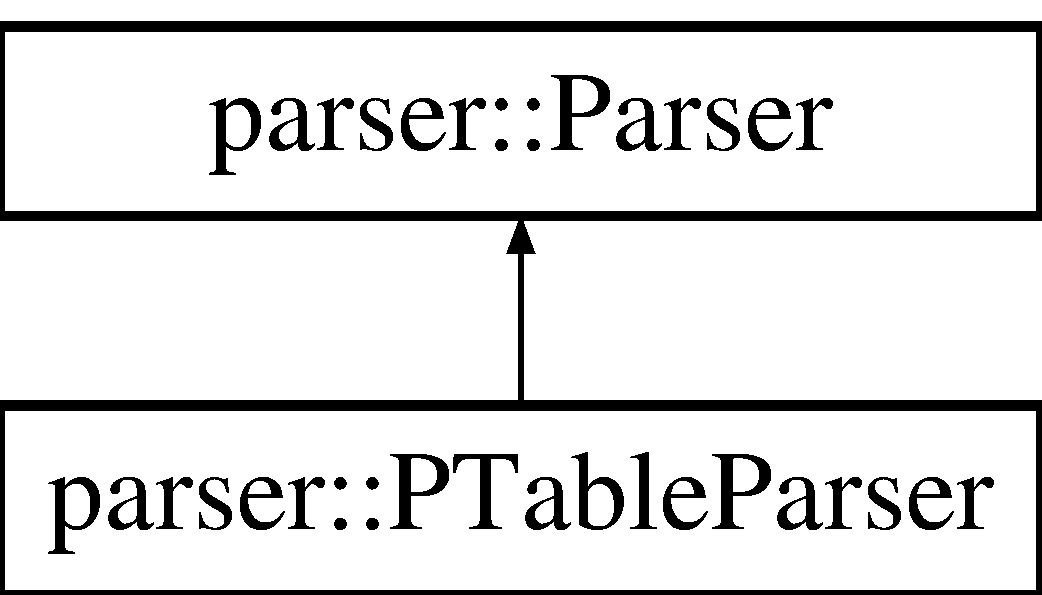
\includegraphics[height=2.000000cm]{da/d8c/classparser_1_1PTableParser}
\end{center}
\end{figure}
\subsection*{\-Public \-Member \-Functions}
\begin{DoxyCompactItemize}
\item 
\hyperlink{classparser_1_1PTableParser_a983ee5c9e9867bfcf82f38e701d3c546}{\-P\-Table\-Parser} ()
\begin{DoxyCompactList}\small\item\em \-Default constructor. \end{DoxyCompactList}\item 
virtual \hyperlink{classparser_1_1PTableParser_ae825bde72b66deb0ee4308ce3c7d100d}{$\sim$\-P\-Table\-Parser} ()
\item 
std\-::vector$<$ std\-::vector\*
$<$ std\-::string $>$ $>$ \hyperlink{classparser_1_1PTableParser_a6efa9956575713877360af5cb41b2e86}{parse} (std\-::string, std\-::vector$<$ std\-::vector$<$ std\-::string $>$ $>$)
\begin{DoxyCompactList}\small\item\em \-This parses the \-Parse \-Table \-X\-M\-L file and fills in the parse table. \end{DoxyCompactList}\end{DoxyCompactItemize}
\subsection*{\-Private \-Member \-Functions}
\begin{DoxyCompactItemize}
\item 
void \hyperlink{classparser_1_1PTableParser_ae20dc625548fbf58a387fa8dfee100ef}{parse\-Row} (\-Ti\-Xml\-Element $\ast$)
\begin{DoxyCompactList}\small\item\em \-Parses one row of the \-X\-M\-L file and fills it in the table. \end{DoxyCompactList}\end{DoxyCompactItemize}
\subsection*{\-Private \-Attributes}
\begin{DoxyCompactItemize}
\item 
std\-::vector$<$ std\-::vector\*
$<$ std\-::string $>$ $>$ \hyperlink{classparser_1_1PTableParser_a7190cd2dc71301c0164bbaacabf07942}{p\-Table\-\_\-}
\end{DoxyCompactItemize}


\subsection{\-Constructor \& \-Destructor \-Documentation}
\hypertarget{classparser_1_1PTableParser_a983ee5c9e9867bfcf82f38e701d3c546}{\index{parser\-::\-P\-Table\-Parser@{parser\-::\-P\-Table\-Parser}!\-P\-Table\-Parser@{\-P\-Table\-Parser}}
\index{\-P\-Table\-Parser@{\-P\-Table\-Parser}!parser::PTableParser@{parser\-::\-P\-Table\-Parser}}
\subsubsection[{\-P\-Table\-Parser}]{\setlength{\rightskip}{0pt plus 5cm}{\bf parser\-::\-P\-Table\-Parser\-::\-P\-Table\-Parser} (
\begin{DoxyParamCaption}
{}
\end{DoxyParamCaption}
)}}\label{da/d8c/classparser_1_1PTableParser_a983ee5c9e9867bfcf82f38e701d3c546}


\-Default constructor. 

\hypertarget{classparser_1_1PTableParser_ae825bde72b66deb0ee4308ce3c7d100d}{\index{parser\-::\-P\-Table\-Parser@{parser\-::\-P\-Table\-Parser}!$\sim$\-P\-Table\-Parser@{$\sim$\-P\-Table\-Parser}}
\index{$\sim$\-P\-Table\-Parser@{$\sim$\-P\-Table\-Parser}!parser::PTableParser@{parser\-::\-P\-Table\-Parser}}
\subsubsection[{$\sim$\-P\-Table\-Parser}]{\setlength{\rightskip}{0pt plus 5cm}virtual {\bf parser\-::\-P\-Table\-Parser\-::$\sim$\-P\-Table\-Parser} (
\begin{DoxyParamCaption}
{}
\end{DoxyParamCaption}
)\hspace{0.3cm}{\ttfamily  \mbox{[}virtual\mbox{]}}}}\label{da/d8c/classparser_1_1PTableParser_ae825bde72b66deb0ee4308ce3c7d100d}


\subsection{\-Member \-Function \-Documentation}
\hypertarget{classparser_1_1PTableParser_a6efa9956575713877360af5cb41b2e86}{\index{parser\-::\-P\-Table\-Parser@{parser\-::\-P\-Table\-Parser}!parse@{parse}}
\index{parse@{parse}!parser::PTableParser@{parser\-::\-P\-Table\-Parser}}
\subsubsection[{parse}]{\setlength{\rightskip}{0pt plus 5cm}std\-::vector$<$std\-::vector$<$std\-::string$>$ $>$ {\bf parser\-::\-P\-Table\-Parser\-::parse} (
\begin{DoxyParamCaption}
\item[{std\-::string}]{, }
\item[{std\-::vector$<$ std\-::vector$<$ std\-::string $>$ $>$}]{}
\end{DoxyParamCaption}
)}}\label{da/d8c/classparser_1_1PTableParser_a6efa9956575713877360af5cb41b2e86}


\-This parses the \-Parse \-Table \-X\-M\-L file and fills in the parse table. 

\hypertarget{classparser_1_1PTableParser_ae20dc625548fbf58a387fa8dfee100ef}{\index{parser\-::\-P\-Table\-Parser@{parser\-::\-P\-Table\-Parser}!parse\-Row@{parse\-Row}}
\index{parse\-Row@{parse\-Row}!parser::PTableParser@{parser\-::\-P\-Table\-Parser}}
\subsubsection[{parse\-Row}]{\setlength{\rightskip}{0pt plus 5cm}void {\bf parser\-::\-P\-Table\-Parser\-::parse\-Row} (
\begin{DoxyParamCaption}
\item[{\-Ti\-Xml\-Element $\ast$}]{}
\end{DoxyParamCaption}
)\hspace{0.3cm}{\ttfamily  \mbox{[}private\mbox{]}}}}\label{da/d8c/classparser_1_1PTableParser_ae20dc625548fbf58a387fa8dfee100ef}


\-Parses one row of the \-X\-M\-L file and fills it in the table. 



\subsection{\-Member \-Data \-Documentation}
\hypertarget{classparser_1_1PTableParser_a7190cd2dc71301c0164bbaacabf07942}{\index{parser\-::\-P\-Table\-Parser@{parser\-::\-P\-Table\-Parser}!p\-Table\-\_\-@{p\-Table\-\_\-}}
\index{p\-Table\-\_\-@{p\-Table\-\_\-}!parser::PTableParser@{parser\-::\-P\-Table\-Parser}}
\subsubsection[{p\-Table\-\_\-}]{\setlength{\rightskip}{0pt plus 5cm}std\-::vector$<$std\-::vector$<$std\-::string$>$ $>$ {\bf parser\-::\-P\-Table\-Parser\-::p\-Table\-\_\-}\hspace{0.3cm}{\ttfamily  \mbox{[}private\mbox{]}}}}\label{da/d8c/classparser_1_1PTableParser_a7190cd2dc71301c0164bbaacabf07942}


\-The documentation for this class was generated from the following file\-:\begin{DoxyCompactItemize}
\item 
src/\hyperlink{PTableParser_8h}{\-P\-Table\-Parser.\-h}\end{DoxyCompactItemize}

\hypertarget{classPDA_1_1State}{\section{P\-D\-A\-:\-:State Class Reference}
\label{classPDA_1_1State}\index{P\-D\-A\-::\-State@{P\-D\-A\-::\-State}}
}


{\ttfamily \#include $<$State.\-h$>$}

\subsection*{Public Member Functions}
\begin{DoxyCompactItemize}
\item 
\hyperlink{classPDA_1_1State_a2d91cf0f7a8de4153abf523f70f72c89}{State} ()
\begin{DoxyCompactList}\small\item\em A default constructor. \end{DoxyCompactList}\item 
\hyperlink{classPDA_1_1State_a70be0ec0f495a76b2dd7858885d784a3}{State} (std\-::string n)
\begin{DoxyCompactList}\small\item\em A specified constructor. \end{DoxyCompactList}\item 
virtual \hyperlink{classPDA_1_1State_a2c301a0f1ba94a1780f016fd6fab17d0}{$\sim$\-State} ()
\begin{DoxyCompactList}\small\item\em Default destructor. \end{DoxyCompactList}\item 
std\-::string \hyperlink{classPDA_1_1State_a703a7b3cb61ffc9bd19c4f161c5bb852}{get\-\_\-name} ()
\begin{DoxyCompactList}\small\item\em A function giving the name of the state. \end{DoxyCompactList}\item 
void \hyperlink{classPDA_1_1State_a3d89cda9ad229bebb25ef256e3470ec8}{add\-\_\-transition} (char input, std\-::string top\-\_\-of\-\_\-stack, std\-::string state, std\-::vector$<$ std\-::string $>$ stack\-\_\-operations)
\begin{DoxyCompactList}\small\item\em A function used to add a transition to a state. \end{DoxyCompactList}\item 
std\-::vector$<$ std\-::pair\\*
$<$ std\-::string, std\-::vector\\*
$<$ std\-::string $>$ $>$ $>$ \hyperlink{classPDA_1_1State_af5d878651060daa40b2259531d1df111}{simulate} (char input, std\-::string top\-\_\-of\-\_\-stack)
\begin{DoxyCompactList}\small\item\em A function returning all the states you can transition to and their stacks given a certain input. \end{DoxyCompactList}\item 
void \hyperlink{classPDA_1_1State_afd437b030a253440225b75695f8ccf90}{print\-\_\-transitions} ()
\begin{DoxyCompactList}\small\item\em A function neatly printing out the transitions. \end{DoxyCompactList}\item 
std\-::multimap$<$ std\-::pair$<$ char, \\*
std\-::string $>$, std\-::pair\\*
$<$ std\-::string, std\-::vector\\*
$<$ std\-::string $>$ $>$ $>$ \hyperlink{classPDA_1_1State_af55439fad25308b084feb62eeaf3b7a2}{get\-\_\-transitions} ()
\begin{DoxyCompactList}\small\item\em A function returning the whole transition map. \end{DoxyCompactList}\end{DoxyCompactItemize}
\subsection*{Private Attributes}
\begin{DoxyCompactItemize}
\item 
std\-::string \hyperlink{classPDA_1_1State_afbfeb988281f28afbb9a0718e8e4eb67}{statename}
\item 
std\-::multimap$<$ std\-::pair$<$ char, \\*
std\-::string $>$, std\-::pair\\*
$<$ std\-::string, std\-::vector\\*
$<$ std\-::string $>$ $>$ $>$ \hyperlink{classPDA_1_1State_abbe5635de165a5a202ba1eb31ee61af1}{transitions}
\begin{DoxyCompactList}\small\item\em A string with the name of the state. \end{DoxyCompactList}\end{DoxyCompactItemize}


\subsection{Constructor \& Destructor Documentation}
\hypertarget{classPDA_1_1State_a2d91cf0f7a8de4153abf523f70f72c89}{\index{P\-D\-A\-::\-State@{P\-D\-A\-::\-State}!State@{State}}
\index{State@{State}!PDA::State@{P\-D\-A\-::\-State}}
\subsubsection[{State}]{\setlength{\rightskip}{0pt plus 5cm}P\-D\-A\-::\-State\-::\-State (
\begin{DoxyParamCaption}
{}
\end{DoxyParamCaption}
)}}\label{classPDA_1_1State_a2d91cf0f7a8de4153abf523f70f72c89}


A default constructor. 

\hypertarget{classPDA_1_1State_a70be0ec0f495a76b2dd7858885d784a3}{\index{P\-D\-A\-::\-State@{P\-D\-A\-::\-State}!State@{State}}
\index{State@{State}!PDA::State@{P\-D\-A\-::\-State}}
\subsubsection[{State}]{\setlength{\rightskip}{0pt plus 5cm}P\-D\-A\-::\-State\-::\-State (
\begin{DoxyParamCaption}
\item[{std\-::string}]{n}
\end{DoxyParamCaption}
)}}\label{classPDA_1_1State_a70be0ec0f495a76b2dd7858885d784a3}


A specified constructor. 


\begin{DoxyParams}{Parameters}
{\em n} & The name of the state. \\
\hline
\end{DoxyParams}
\hypertarget{classPDA_1_1State_a2c301a0f1ba94a1780f016fd6fab17d0}{\index{P\-D\-A\-::\-State@{P\-D\-A\-::\-State}!$\sim$\-State@{$\sim$\-State}}
\index{$\sim$\-State@{$\sim$\-State}!PDA::State@{P\-D\-A\-::\-State}}
\subsubsection[{$\sim$\-State}]{\setlength{\rightskip}{0pt plus 5cm}virtual P\-D\-A\-::\-State\-::$\sim$\-State (
\begin{DoxyParamCaption}
{}
\end{DoxyParamCaption}
)\hspace{0.3cm}{\ttfamily [virtual]}}}\label{classPDA_1_1State_a2c301a0f1ba94a1780f016fd6fab17d0}


Default destructor. 



\subsection{Member Function Documentation}
\hypertarget{classPDA_1_1State_a3d89cda9ad229bebb25ef256e3470ec8}{\index{P\-D\-A\-::\-State@{P\-D\-A\-::\-State}!add\-\_\-transition@{add\-\_\-transition}}
\index{add\-\_\-transition@{add\-\_\-transition}!PDA::State@{P\-D\-A\-::\-State}}
\subsubsection[{add\-\_\-transition}]{\setlength{\rightskip}{0pt plus 5cm}void P\-D\-A\-::\-State\-::add\-\_\-transition (
\begin{DoxyParamCaption}
\item[{char}]{input, }
\item[{std\-::string}]{top\-\_\-of\-\_\-stack, }
\item[{std\-::string}]{state, }
\item[{std\-::vector$<$ std\-::string $>$}]{stack\-\_\-operations}
\end{DoxyParamCaption}
)}}\label{classPDA_1_1State_a3d89cda9ad229bebb25ef256e3470ec8}


A function used to add a transition to a state. 


\begin{DoxyParams}{Parameters}
{\em input} & The input symbol on which the state should transition. \\
\hline
{\em top\-\_\-of\-\_\-stack} & The symbol that should be on top of the stack when transitioning. \\
\hline
{\em state} & The name of the state you want to transition to. \\
\hline
{\em stack\-\_\-operations} & A vector containing operations that should be run on the stack. \\
\hline
\end{DoxyParams}
\hypertarget{classPDA_1_1State_a703a7b3cb61ffc9bd19c4f161c5bb852}{\index{P\-D\-A\-::\-State@{P\-D\-A\-::\-State}!get\-\_\-name@{get\-\_\-name}}
\index{get\-\_\-name@{get\-\_\-name}!PDA::State@{P\-D\-A\-::\-State}}
\subsubsection[{get\-\_\-name}]{\setlength{\rightskip}{0pt plus 5cm}std\-::string P\-D\-A\-::\-State\-::get\-\_\-name (
\begin{DoxyParamCaption}
{}
\end{DoxyParamCaption}
)}}\label{classPDA_1_1State_a703a7b3cb61ffc9bd19c4f161c5bb852}


A function giving the name of the state. 

\begin{DoxyReturn}{Returns}
It returns a string with the name of the state. 
\end{DoxyReturn}
\hypertarget{classPDA_1_1State_af55439fad25308b084feb62eeaf3b7a2}{\index{P\-D\-A\-::\-State@{P\-D\-A\-::\-State}!get\-\_\-transitions@{get\-\_\-transitions}}
\index{get\-\_\-transitions@{get\-\_\-transitions}!PDA::State@{P\-D\-A\-::\-State}}
\subsubsection[{get\-\_\-transitions}]{\setlength{\rightskip}{0pt plus 5cm}std\-::multimap$<$std\-::pair$<$char, std\-::string$>$, std\-::pair$<$std\-::string, std\-::vector$<$std\-::string$>$ $>$ $>$ P\-D\-A\-::\-State\-::get\-\_\-transitions (
\begin{DoxyParamCaption}
{}
\end{DoxyParamCaption}
)}}\label{classPDA_1_1State_af55439fad25308b084feb62eeaf3b7a2}


A function returning the whole transition map. 

\begin{DoxyReturn}{Returns}
A multimap containing the input symbols and corresponding transition info. 
\end{DoxyReturn}
\hypertarget{classPDA_1_1State_afd437b030a253440225b75695f8ccf90}{\index{P\-D\-A\-::\-State@{P\-D\-A\-::\-State}!print\-\_\-transitions@{print\-\_\-transitions}}
\index{print\-\_\-transitions@{print\-\_\-transitions}!PDA::State@{P\-D\-A\-::\-State}}
\subsubsection[{print\-\_\-transitions}]{\setlength{\rightskip}{0pt plus 5cm}void P\-D\-A\-::\-State\-::print\-\_\-transitions (
\begin{DoxyParamCaption}
{}
\end{DoxyParamCaption}
)}}\label{classPDA_1_1State_afd437b030a253440225b75695f8ccf90}


A function neatly printing out the transitions. 

\hypertarget{classPDA_1_1State_af5d878651060daa40b2259531d1df111}{\index{P\-D\-A\-::\-State@{P\-D\-A\-::\-State}!simulate@{simulate}}
\index{simulate@{simulate}!PDA::State@{P\-D\-A\-::\-State}}
\subsubsection[{simulate}]{\setlength{\rightskip}{0pt plus 5cm}std\-::vector$<$std\-::pair$<$std\-::string, std\-::vector$<$std\-::string$>$ $>$ $>$ P\-D\-A\-::\-State\-::simulate (
\begin{DoxyParamCaption}
\item[{char}]{input, }
\item[{std\-::string}]{top\-\_\-of\-\_\-stack}
\end{DoxyParamCaption}
)}}\label{classPDA_1_1State_af5d878651060daa40b2259531d1df111}


A function returning all the states you can transition to and their stacks given a certain input. 


\begin{DoxyParams}{Parameters}
{\em input} & The char that is read to transition. \\
\hline
{\em top\-\_\-of\-\_\-stack} & The current top of the stack. \\
\hline
\end{DoxyParams}
\begin{DoxyReturn}{Returns}
A vector containing pairs with the name of the state you can go to and the operations of the stack you should run then. 
\end{DoxyReturn}


\subsection{Member Data Documentation}
\hypertarget{classPDA_1_1State_afbfeb988281f28afbb9a0718e8e4eb67}{\index{P\-D\-A\-::\-State@{P\-D\-A\-::\-State}!statename@{statename}}
\index{statename@{statename}!PDA::State@{P\-D\-A\-::\-State}}
\subsubsection[{statename}]{\setlength{\rightskip}{0pt plus 5cm}std\-::string P\-D\-A\-::\-State\-::statename\hspace{0.3cm}{\ttfamily [private]}}}\label{classPDA_1_1State_afbfeb988281f28afbb9a0718e8e4eb67}
\hypertarget{classPDA_1_1State_abbe5635de165a5a202ba1eb31ee61af1}{\index{P\-D\-A\-::\-State@{P\-D\-A\-::\-State}!transitions@{transitions}}
\index{transitions@{transitions}!PDA::State@{P\-D\-A\-::\-State}}
\subsubsection[{transitions}]{\setlength{\rightskip}{0pt plus 5cm}std\-::multimap$<$std\-::pair$<$char, std\-::string$>$, std\-::pair$<$std\-::string, std\-::vector$<$std\-::string$>$ $>$ $>$ P\-D\-A\-::\-State\-::transitions\hspace{0.3cm}{\ttfamily [private]}}}\label{classPDA_1_1State_abbe5635de165a5a202ba1eb31ee61af1}


A string with the name of the state. 



The documentation for this class was generated from the following file\-:\begin{DoxyCompactItemize}
\item 
src/\hyperlink{State_8h}{State.\-h}\end{DoxyCompactItemize}

\hypertarget{classTM_1_1TapeSymbol}{\section{\-T\-M\-:\-:\-Tape\-Symbol \-Class \-Reference}
\label{d8/d62/classTM_1_1TapeSymbol}\index{\-T\-M\-::\-Tape\-Symbol@{\-T\-M\-::\-Tape\-Symbol}}
}


{\ttfamily \#include $<$\-Tape\-Symbol.\-h$>$}

\subsection*{\-Public \-Member \-Functions}
\begin{DoxyCompactItemize}
\item 
\hyperlink{classTM_1_1TapeSymbol_a2766ff5c8be461a1936e422dbc21e266}{\-Tape\-Symbol} ()
\begin{DoxyCompactList}\small\item\em \-Default constructor\-: makes a blank \hyperlink{classTM_1_1TapeSymbol}{\-Tape\-Symbol}. \end{DoxyCompactList}\item 
\hyperlink{classTM_1_1TapeSymbol_a5f3591fae790d4eb2e8e209eb727ac0b}{\-Tape\-Symbol} (unsigned int i)
\begin{DoxyCompactList}\small\item\em \-Constructor making an int \hyperlink{classTM_1_1TapeSymbol}{\-Tape\-Symbol}. \end{DoxyCompactList}\item 
\hyperlink{classTM_1_1TapeSymbol_abc65d6f09ccdfa19cfbfc14772dd9068}{\-Tape\-Symbol} (std\-::string c)
\begin{DoxyCompactList}\small\item\em \-Constructor making a character \hyperlink{classTM_1_1TapeSymbol}{\-Tape\-Symbol}. \end{DoxyCompactList}\item 
\hyperlink{classTM_1_1TapeSymbol}{\-Tape\-Symbol} \& \hyperlink{classTM_1_1TapeSymbol_ae71634efcc0f0ca8c8d02d3f2b59a76c}{operator=} (const \hyperlink{classTM_1_1TapeSymbol}{\-Tape\-Symbol} \&ts)
\begin{DoxyCompactList}\small\item\em \-Assignment operator. \end{DoxyCompactList}\item 
bool \hyperlink{classTM_1_1TapeSymbol_a303e737aa42371bd09e85407e36fed56}{is\-Blank} () const 
\begin{DoxyCompactList}\small\item\em \-A function checking if this is a blank. \end{DoxyCompactList}\end{DoxyCompactItemize}
\subsection*{\-Private \-Attributes}
\begin{DoxyCompactItemize}
\item 
unsigned int \hyperlink{classTM_1_1TapeSymbol_a09b69817f96736cc1f958d6c2d2aa2b0}{integer\-\_\-}
\item 
std\-::string \hyperlink{classTM_1_1TapeSymbol_a86066d23f5c51d788d039ccc50aa44a6}{character\-\_\-}
\begin{DoxyCompactList}\small\item\em integer value; \end{DoxyCompactList}\item 
\hyperlink{namespaceTM_ac5907d46a678a9a9fe237dce1768dbad}{\-Type} \hyperlink{classTM_1_1TapeSymbol_af84d020bd2a06906fc7bb461cf16fb14}{select\-\_\-}
\begin{DoxyCompactList}\small\item\em character value \end{DoxyCompactList}\end{DoxyCompactItemize}
\subsection*{\-Friends}
\begin{DoxyCompactItemize}
\item 
bool \hyperlink{classTM_1_1TapeSymbol_a0eb718edb9457b586f4e200b7eddfdf3}{operator==} (\hyperlink{classTM_1_1TapeSymbol}{\-Tape\-Symbol} t, \hyperlink{classTM_1_1TapeSymbol}{\-Tape\-Symbol} ts)
\begin{DoxyCompactList}\small\item\em \-Comparison operator. \end{DoxyCompactList}\item 
std\-::ostream \& \hyperlink{classTM_1_1TapeSymbol_ae2fd50d93deb1efc1b7e831b8ec43d8c}{operator$<$$<$} (std\-::ostream \&out, \hyperlink{classTM_1_1TapeSymbol}{\-Tape\-Symbol} \&ts)
\begin{DoxyCompactList}\small\item\em output operator \end{DoxyCompactList}\end{DoxyCompactItemize}


\subsection{\-Constructor \& \-Destructor \-Documentation}
\hypertarget{classTM_1_1TapeSymbol_a2766ff5c8be461a1936e422dbc21e266}{\index{\-T\-M\-::\-Tape\-Symbol@{\-T\-M\-::\-Tape\-Symbol}!\-Tape\-Symbol@{\-Tape\-Symbol}}
\index{\-Tape\-Symbol@{\-Tape\-Symbol}!TM::TapeSymbol@{\-T\-M\-::\-Tape\-Symbol}}
\subsubsection[{\-Tape\-Symbol}]{\setlength{\rightskip}{0pt plus 5cm}{\bf \-T\-M\-::\-Tape\-Symbol\-::\-Tape\-Symbol} (
\begin{DoxyParamCaption}
{}
\end{DoxyParamCaption}
)}}\label{d8/d62/classTM_1_1TapeSymbol_a2766ff5c8be461a1936e422dbc21e266}


\-Default constructor\-: makes a blank \hyperlink{classTM_1_1TapeSymbol}{\-Tape\-Symbol}. 

\hypertarget{classTM_1_1TapeSymbol_a5f3591fae790d4eb2e8e209eb727ac0b}{\index{\-T\-M\-::\-Tape\-Symbol@{\-T\-M\-::\-Tape\-Symbol}!\-Tape\-Symbol@{\-Tape\-Symbol}}
\index{\-Tape\-Symbol@{\-Tape\-Symbol}!TM::TapeSymbol@{\-T\-M\-::\-Tape\-Symbol}}
\subsubsection[{\-Tape\-Symbol}]{\setlength{\rightskip}{0pt plus 5cm}{\bf \-T\-M\-::\-Tape\-Symbol\-::\-Tape\-Symbol} (
\begin{DoxyParamCaption}
\item[{unsigned int}]{i}
\end{DoxyParamCaption}
)}}\label{d8/d62/classTM_1_1TapeSymbol_a5f3591fae790d4eb2e8e209eb727ac0b}


\-Constructor making an int \hyperlink{classTM_1_1TapeSymbol}{\-Tape\-Symbol}. 

\hypertarget{classTM_1_1TapeSymbol_abc65d6f09ccdfa19cfbfc14772dd9068}{\index{\-T\-M\-::\-Tape\-Symbol@{\-T\-M\-::\-Tape\-Symbol}!\-Tape\-Symbol@{\-Tape\-Symbol}}
\index{\-Tape\-Symbol@{\-Tape\-Symbol}!TM::TapeSymbol@{\-T\-M\-::\-Tape\-Symbol}}
\subsubsection[{\-Tape\-Symbol}]{\setlength{\rightskip}{0pt plus 5cm}{\bf \-T\-M\-::\-Tape\-Symbol\-::\-Tape\-Symbol} (
\begin{DoxyParamCaption}
\item[{std\-::string}]{c}
\end{DoxyParamCaption}
)}}\label{d8/d62/classTM_1_1TapeSymbol_abc65d6f09ccdfa19cfbfc14772dd9068}


\-Constructor making a character \hyperlink{classTM_1_1TapeSymbol}{\-Tape\-Symbol}. 



\subsection{\-Member \-Function \-Documentation}
\hypertarget{classTM_1_1TapeSymbol_a303e737aa42371bd09e85407e36fed56}{\index{\-T\-M\-::\-Tape\-Symbol@{\-T\-M\-::\-Tape\-Symbol}!is\-Blank@{is\-Blank}}
\index{is\-Blank@{is\-Blank}!TM::TapeSymbol@{\-T\-M\-::\-Tape\-Symbol}}
\subsubsection[{is\-Blank}]{\setlength{\rightskip}{0pt plus 5cm}bool {\bf \-T\-M\-::\-Tape\-Symbol\-::is\-Blank} (
\begin{DoxyParamCaption}
{}
\end{DoxyParamCaption}
) const}}\label{d8/d62/classTM_1_1TapeSymbol_a303e737aa42371bd09e85407e36fed56}


\-A function checking if this is a blank. 

\hypertarget{classTM_1_1TapeSymbol_ae71634efcc0f0ca8c8d02d3f2b59a76c}{\index{\-T\-M\-::\-Tape\-Symbol@{\-T\-M\-::\-Tape\-Symbol}!operator=@{operator=}}
\index{operator=@{operator=}!TM::TapeSymbol@{\-T\-M\-::\-Tape\-Symbol}}
\subsubsection[{operator=}]{\setlength{\rightskip}{0pt plus 5cm}{\bf \-Tape\-Symbol}\& \-T\-M\-::\-Tape\-Symbol\-::operator= (
\begin{DoxyParamCaption}
\item[{const {\bf \-Tape\-Symbol} \&}]{ts}
\end{DoxyParamCaption}
)}}\label{d8/d62/classTM_1_1TapeSymbol_ae71634efcc0f0ca8c8d02d3f2b59a76c}


\-Assignment operator. 



\subsection{\-Friends \-And \-Related \-Function \-Documentation}
\hypertarget{classTM_1_1TapeSymbol_ae2fd50d93deb1efc1b7e831b8ec43d8c}{\index{\-T\-M\-::\-Tape\-Symbol@{\-T\-M\-::\-Tape\-Symbol}!operator$<$$<$@{operator$<$$<$}}
\index{operator$<$$<$@{operator$<$$<$}!TM::TapeSymbol@{\-T\-M\-::\-Tape\-Symbol}}
\subsubsection[{operator$<$$<$}]{\setlength{\rightskip}{0pt plus 5cm}std\-::ostream\& operator$<$$<$ (
\begin{DoxyParamCaption}
\item[{std\-::ostream \&}]{out, }
\item[{{\bf \-Tape\-Symbol} \&}]{ts}
\end{DoxyParamCaption}
)\hspace{0.3cm}{\ttfamily  \mbox{[}friend\mbox{]}}}}\label{d8/d62/classTM_1_1TapeSymbol_ae2fd50d93deb1efc1b7e831b8ec43d8c}


output operator 

\hypertarget{classTM_1_1TapeSymbol_a0eb718edb9457b586f4e200b7eddfdf3}{\index{\-T\-M\-::\-Tape\-Symbol@{\-T\-M\-::\-Tape\-Symbol}!operator==@{operator==}}
\index{operator==@{operator==}!TM::TapeSymbol@{\-T\-M\-::\-Tape\-Symbol}}
\subsubsection[{operator==}]{\setlength{\rightskip}{0pt plus 5cm}bool operator== (
\begin{DoxyParamCaption}
\item[{{\bf \-Tape\-Symbol}}]{t, }
\item[{{\bf \-Tape\-Symbol}}]{ts}
\end{DoxyParamCaption}
)\hspace{0.3cm}{\ttfamily  \mbox{[}friend\mbox{]}}}}\label{d8/d62/classTM_1_1TapeSymbol_a0eb718edb9457b586f4e200b7eddfdf3}


\-Comparison operator. 



\subsection{\-Member \-Data \-Documentation}
\hypertarget{classTM_1_1TapeSymbol_a86066d23f5c51d788d039ccc50aa44a6}{\index{\-T\-M\-::\-Tape\-Symbol@{\-T\-M\-::\-Tape\-Symbol}!character\-\_\-@{character\-\_\-}}
\index{character\-\_\-@{character\-\_\-}!TM::TapeSymbol@{\-T\-M\-::\-Tape\-Symbol}}
\subsubsection[{character\-\_\-}]{\setlength{\rightskip}{0pt plus 5cm}std\-::string {\bf \-T\-M\-::\-Tape\-Symbol\-::character\-\_\-}\hspace{0.3cm}{\ttfamily  \mbox{[}private\mbox{]}}}}\label{d8/d62/classTM_1_1TapeSymbol_a86066d23f5c51d788d039ccc50aa44a6}


integer value; 

\hypertarget{classTM_1_1TapeSymbol_a09b69817f96736cc1f958d6c2d2aa2b0}{\index{\-T\-M\-::\-Tape\-Symbol@{\-T\-M\-::\-Tape\-Symbol}!integer\-\_\-@{integer\-\_\-}}
\index{integer\-\_\-@{integer\-\_\-}!TM::TapeSymbol@{\-T\-M\-::\-Tape\-Symbol}}
\subsubsection[{integer\-\_\-}]{\setlength{\rightskip}{0pt plus 5cm}unsigned int {\bf \-T\-M\-::\-Tape\-Symbol\-::integer\-\_\-}\hspace{0.3cm}{\ttfamily  \mbox{[}private\mbox{]}}}}\label{d8/d62/classTM_1_1TapeSymbol_a09b69817f96736cc1f958d6c2d2aa2b0}
\hypertarget{classTM_1_1TapeSymbol_af84d020bd2a06906fc7bb461cf16fb14}{\index{\-T\-M\-::\-Tape\-Symbol@{\-T\-M\-::\-Tape\-Symbol}!select\-\_\-@{select\-\_\-}}
\index{select\-\_\-@{select\-\_\-}!TM::TapeSymbol@{\-T\-M\-::\-Tape\-Symbol}}
\subsubsection[{select\-\_\-}]{\setlength{\rightskip}{0pt plus 5cm}{\bf \-Type} {\bf \-T\-M\-::\-Tape\-Symbol\-::select\-\_\-}\hspace{0.3cm}{\ttfamily  \mbox{[}private\mbox{]}}}}\label{d8/d62/classTM_1_1TapeSymbol_af84d020bd2a06906fc7bb461cf16fb14}


character value 



\-The documentation for this class was generated from the following file\-:\begin{DoxyCompactItemize}
\item 
src/\hyperlink{TapeSymbol_8h}{\-Tape\-Symbol.\-h}\end{DoxyCompactItemize}

\hypertarget{classparser_1_1TMParser}{\section{parser\-:\-:\-T\-M\-Parser \-Class \-Reference}
\label{d0/d6a/classparser_1_1TMParser}\index{parser\-::\-T\-M\-Parser@{parser\-::\-T\-M\-Parser}}
}


{\ttfamily \#include $<$\-T\-M\-Parser.\-h$>$}

\subsection*{\-Public \-Member \-Functions}
\begin{DoxyCompactItemize}
\item 
\hyperlink{classparser_1_1TMParser_a7449386b475a892715af85ad31fa0015}{\-T\-M\-Parser} (std\-::string)
\begin{DoxyCompactList}\small\item\em \-Main constructor for \hyperlink{classparser_1_1TMParser}{\-T\-M\-Parser}. \-This will parse the parameter file and save the info in its members. \end{DoxyCompactList}\item 
virtual \hyperlink{classparser_1_1TMParser_a7dc139954aaa9f7bacd0c433fbbd3519}{$\sim$\-T\-M\-Parser} ()
\item 
std\-::string \hyperlink{classparser_1_1TMParser_a041286999146f207f2f127fdedd19403}{get\-Init\-Input} () const 
\item 
std\-::vector$<$ \hyperlink{namespaceTM_a852554502c474841ede5736b807839ff}{\-T\-M\-::\-State\-Name} $>$ \hyperlink{classparser_1_1TMParser_a218e4bf57cad53fa565cbe7bc9103181}{get\-States} () const 
\item 
std\-::vector$<$ \hyperlink{namespaceTM_a87460339f40338ea4e37433443965554}{\-T\-M\-::\-Production} $>$ \hyperlink{classparser_1_1TMParser_a582cb825725c2d6fb69dead1ce168065}{get\-Productions} () const 
\end{DoxyCompactItemize}
\subsection*{\-Private \-Member \-Functions}
\begin{DoxyCompactItemize}
\item 
void \hyperlink{classparser_1_1TMParser_aadb9e65b789495fc3dde6132d61ff53f}{parse\-States} (std\-::string, std\-::size\-\_\-t)
\item 
void \hyperlink{classparser_1_1TMParser_af238e382d917a1e09438d3d971dc375c}{parse\-Init\-Input} (std\-::string, std\-::size\-\_\-t)
\item 
void \hyperlink{classparser_1_1TMParser_a58ffe167af0cfb98089dafca94a8f891}{parse\-Production} (std\-::string)
\item 
void \hyperlink{classparser_1_1TMParser_a0f0fa124f3929c854f764914f644b6f2}{iterator\-Check} (std\-::string\-::iterator \&, char) const 
\end{DoxyCompactItemize}
\subsection*{\-Private \-Attributes}
\begin{DoxyCompactItemize}
\item 
std\-::string \hyperlink{classparser_1_1TMParser_acecddd2b0a5413a91c7744090e582e33}{init\-Input\-\_\-}
\begin{DoxyCompactList}\small\item\em \-Initial input for the \-Turing \-Machine. \end{DoxyCompactList}\item 
std\-::vector$<$ \hyperlink{namespaceTM_a852554502c474841ede5736b807839ff}{\-T\-M\-::\-State\-Name} $>$ \hyperlink{classparser_1_1TMParser_a8214139fde7f1051bec5c9b786319d1d}{states\-\_\-}
\begin{DoxyCompactList}\small\item\em \-All states for the \-Turing \-Machine. \end{DoxyCompactList}\item 
std\-::vector$<$ \hyperlink{namespaceTM_a87460339f40338ea4e37433443965554}{\-T\-M\-::\-Production} $>$ \hyperlink{classparser_1_1TMParser_a7948f791b173d8444cfdf47398f2202e}{productions\-\_\-}
\begin{DoxyCompactList}\small\item\em \-All productions for the \-Turing \-Machine. \end{DoxyCompactList}\end{DoxyCompactItemize}
\subsection*{\-Friends}
\begin{DoxyCompactItemize}
\item 
std\-::ostream \& \hyperlink{classparser_1_1TMParser_a4ff9f93f95023ec45081a5336b6b5738}{operator$<$$<$} (std\-::ostream \&out, \hyperlink{classparser_1_1TMParser}{\-T\-M\-Parser} \&tmp)
\end{DoxyCompactItemize}


\subsection{\-Constructor \& \-Destructor \-Documentation}
\hypertarget{classparser_1_1TMParser_a7449386b475a892715af85ad31fa0015}{\index{parser\-::\-T\-M\-Parser@{parser\-::\-T\-M\-Parser}!\-T\-M\-Parser@{\-T\-M\-Parser}}
\index{\-T\-M\-Parser@{\-T\-M\-Parser}!parser::TMParser@{parser\-::\-T\-M\-Parser}}
\subsubsection[{\-T\-M\-Parser}]{\setlength{\rightskip}{0pt plus 5cm}{\bf parser\-::\-T\-M\-Parser\-::\-T\-M\-Parser} (
\begin{DoxyParamCaption}
\item[{std\-::string}]{}
\end{DoxyParamCaption}
)}}\label{d0/d6a/classparser_1_1TMParser_a7449386b475a892715af85ad31fa0015}


\-Main constructor for \hyperlink{classparser_1_1TMParser}{\-T\-M\-Parser}. \-This will parse the parameter file and save the info in its members. 


\begin{DoxyParams}{\-Parameters}
{\em file} & \-The file that needs to be parsed. \\
\hline
\end{DoxyParams}
\hypertarget{classparser_1_1TMParser_a7dc139954aaa9f7bacd0c433fbbd3519}{\index{parser\-::\-T\-M\-Parser@{parser\-::\-T\-M\-Parser}!$\sim$\-T\-M\-Parser@{$\sim$\-T\-M\-Parser}}
\index{$\sim$\-T\-M\-Parser@{$\sim$\-T\-M\-Parser}!parser::TMParser@{parser\-::\-T\-M\-Parser}}
\subsubsection[{$\sim$\-T\-M\-Parser}]{\setlength{\rightskip}{0pt plus 5cm}virtual {\bf parser\-::\-T\-M\-Parser\-::$\sim$\-T\-M\-Parser} (
\begin{DoxyParamCaption}
{}
\end{DoxyParamCaption}
)\hspace{0.3cm}{\ttfamily  \mbox{[}virtual\mbox{]}}}}\label{d0/d6a/classparser_1_1TMParser_a7dc139954aaa9f7bacd0c433fbbd3519}


\subsection{\-Member \-Function \-Documentation}
\hypertarget{classparser_1_1TMParser_a041286999146f207f2f127fdedd19403}{\index{parser\-::\-T\-M\-Parser@{parser\-::\-T\-M\-Parser}!get\-Init\-Input@{get\-Init\-Input}}
\index{get\-Init\-Input@{get\-Init\-Input}!parser::TMParser@{parser\-::\-T\-M\-Parser}}
\subsubsection[{get\-Init\-Input}]{\setlength{\rightskip}{0pt plus 5cm}std\-::string {\bf parser\-::\-T\-M\-Parser\-::get\-Init\-Input} (
\begin{DoxyParamCaption}
{}
\end{DoxyParamCaption}
) const}}\label{d0/d6a/classparser_1_1TMParser_a041286999146f207f2f127fdedd19403}
\begin{DoxyReturn}{\-Returns}
initial input for the \-Turing\-Machine. 
\end{DoxyReturn}
\hypertarget{classparser_1_1TMParser_a582cb825725c2d6fb69dead1ce168065}{\index{parser\-::\-T\-M\-Parser@{parser\-::\-T\-M\-Parser}!get\-Productions@{get\-Productions}}
\index{get\-Productions@{get\-Productions}!parser::TMParser@{parser\-::\-T\-M\-Parser}}
\subsubsection[{get\-Productions}]{\setlength{\rightskip}{0pt plus 5cm}std\-::vector$<${\bf \-T\-M\-::\-Production}$>$ {\bf parser\-::\-T\-M\-Parser\-::get\-Productions} (
\begin{DoxyParamCaption}
{}
\end{DoxyParamCaption}
) const}}\label{d0/d6a/classparser_1_1TMParser_a582cb825725c2d6fb69dead1ce168065}
\begin{DoxyReturn}{\-Returns}
all productions for the \-Turing\-Machine. 
\end{DoxyReturn}
\hypertarget{classparser_1_1TMParser_a218e4bf57cad53fa565cbe7bc9103181}{\index{parser\-::\-T\-M\-Parser@{parser\-::\-T\-M\-Parser}!get\-States@{get\-States}}
\index{get\-States@{get\-States}!parser::TMParser@{parser\-::\-T\-M\-Parser}}
\subsubsection[{get\-States}]{\setlength{\rightskip}{0pt plus 5cm}std\-::vector$<${\bf \-T\-M\-::\-State\-Name}$>$ {\bf parser\-::\-T\-M\-Parser\-::get\-States} (
\begin{DoxyParamCaption}
{}
\end{DoxyParamCaption}
) const}}\label{d0/d6a/classparser_1_1TMParser_a218e4bf57cad53fa565cbe7bc9103181}
\begin{DoxyReturn}{\-Returns}
all states for the \-Turing\-Machine. 
\end{DoxyReturn}
\hypertarget{classparser_1_1TMParser_a0f0fa124f3929c854f764914f644b6f2}{\index{parser\-::\-T\-M\-Parser@{parser\-::\-T\-M\-Parser}!iterator\-Check@{iterator\-Check}}
\index{iterator\-Check@{iterator\-Check}!parser::TMParser@{parser\-::\-T\-M\-Parser}}
\subsubsection[{iterator\-Check}]{\setlength{\rightskip}{0pt plus 5cm}void {\bf parser\-::\-T\-M\-Parser\-::iterator\-Check} (
\begin{DoxyParamCaption}
\item[{std\-::string\-::iterator \&}]{, }
\item[{char}]{}
\end{DoxyParamCaption}
) const\hspace{0.3cm}{\ttfamily  \mbox{[}private\mbox{]}}}}\label{d0/d6a/classparser_1_1TMParser_a0f0fa124f3929c854f764914f644b6f2}

\begin{DoxyParams}{\-Parameters}
{\em it2\&} & \-The iterator we need to use in our check. \\
\hline
{\em c} & \-The char the iterator needs to pass. \\
\hline
\end{DoxyParams}
\hypertarget{classparser_1_1TMParser_af238e382d917a1e09438d3d971dc375c}{\index{parser\-::\-T\-M\-Parser@{parser\-::\-T\-M\-Parser}!parse\-Init\-Input@{parse\-Init\-Input}}
\index{parse\-Init\-Input@{parse\-Init\-Input}!parser::TMParser@{parser\-::\-T\-M\-Parser}}
\subsubsection[{parse\-Init\-Input}]{\setlength{\rightskip}{0pt plus 5cm}void {\bf parser\-::\-T\-M\-Parser\-::parse\-Init\-Input} (
\begin{DoxyParamCaption}
\item[{std\-::string}]{, }
\item[{std\-::size\-\_\-t}]{}
\end{DoxyParamCaption}
)\hspace{0.3cm}{\ttfamily  \mbox{[}private\mbox{]}}}}\label{d0/d6a/classparser_1_1TMParser_af238e382d917a1e09438d3d971dc375c}

\begin{DoxyParams}{\-Parameters}
{\em line} & \-The string that contains the initial input. \\
\hline
{\em found} & \-The index where the string \char`\"{}\-I\-N\-I\-T\-I\-A\-L\-\_\-\-I\-N\-P\-U\-T = \char`\"{} begins. \\
\hline
\end{DoxyParams}
\hypertarget{classparser_1_1TMParser_a58ffe167af0cfb98089dafca94a8f891}{\index{parser\-::\-T\-M\-Parser@{parser\-::\-T\-M\-Parser}!parse\-Production@{parse\-Production}}
\index{parse\-Production@{parse\-Production}!parser::TMParser@{parser\-::\-T\-M\-Parser}}
\subsubsection[{parse\-Production}]{\setlength{\rightskip}{0pt plus 5cm}void {\bf parser\-::\-T\-M\-Parser\-::parse\-Production} (
\begin{DoxyParamCaption}
\item[{std\-::string}]{}
\end{DoxyParamCaption}
)\hspace{0.3cm}{\ttfamily  \mbox{[}private\mbox{]}}}}\label{d0/d6a/classparser_1_1TMParser_a58ffe167af0cfb98089dafca94a8f891}

\begin{DoxyParams}{\-Parameters}
{\em line} & \-The string that contains a production. \\
\hline
\end{DoxyParams}
\hypertarget{classparser_1_1TMParser_aadb9e65b789495fc3dde6132d61ff53f}{\index{parser\-::\-T\-M\-Parser@{parser\-::\-T\-M\-Parser}!parse\-States@{parse\-States}}
\index{parse\-States@{parse\-States}!parser::TMParser@{parser\-::\-T\-M\-Parser}}
\subsubsection[{parse\-States}]{\setlength{\rightskip}{0pt plus 5cm}void {\bf parser\-::\-T\-M\-Parser\-::parse\-States} (
\begin{DoxyParamCaption}
\item[{std\-::string}]{, }
\item[{std\-::size\-\_\-t}]{}
\end{DoxyParamCaption}
)\hspace{0.3cm}{\ttfamily  \mbox{[}private\mbox{]}}}}\label{d0/d6a/classparser_1_1TMParser_aadb9e65b789495fc3dde6132d61ff53f}

\begin{DoxyParams}{\-Parameters}
{\em line} & \-The string that contains the states. \\
\hline
{\em found} & \-The index where the string \char`\"{}\-S\-T\-A\-T\-E\-S = \{\char`\"{} begins. \\
\hline
\end{DoxyParams}


\subsection{\-Friends \-And \-Related \-Function \-Documentation}
\hypertarget{classparser_1_1TMParser_a4ff9f93f95023ec45081a5336b6b5738}{\index{parser\-::\-T\-M\-Parser@{parser\-::\-T\-M\-Parser}!operator$<$$<$@{operator$<$$<$}}
\index{operator$<$$<$@{operator$<$$<$}!parser::TMParser@{parser\-::\-T\-M\-Parser}}
\subsubsection[{operator$<$$<$}]{\setlength{\rightskip}{0pt plus 5cm}std\-::ostream\& operator$<$$<$ (
\begin{DoxyParamCaption}
\item[{std\-::ostream \&}]{out, }
\item[{{\bf \-T\-M\-Parser} \&}]{tmp}
\end{DoxyParamCaption}
)\hspace{0.3cm}{\ttfamily  \mbox{[}friend\mbox{]}}}}\label{d0/d6a/classparser_1_1TMParser_a4ff9f93f95023ec45081a5336b6b5738}


\subsection{\-Member \-Data \-Documentation}
\hypertarget{classparser_1_1TMParser_acecddd2b0a5413a91c7744090e582e33}{\index{parser\-::\-T\-M\-Parser@{parser\-::\-T\-M\-Parser}!init\-Input\-\_\-@{init\-Input\-\_\-}}
\index{init\-Input\-\_\-@{init\-Input\-\_\-}!parser::TMParser@{parser\-::\-T\-M\-Parser}}
\subsubsection[{init\-Input\-\_\-}]{\setlength{\rightskip}{0pt plus 5cm}std\-::string {\bf parser\-::\-T\-M\-Parser\-::init\-Input\-\_\-}\hspace{0.3cm}{\ttfamily  \mbox{[}private\mbox{]}}}}\label{d0/d6a/classparser_1_1TMParser_acecddd2b0a5413a91c7744090e582e33}


\-Initial input for the \-Turing \-Machine. 

\hypertarget{classparser_1_1TMParser_a7948f791b173d8444cfdf47398f2202e}{\index{parser\-::\-T\-M\-Parser@{parser\-::\-T\-M\-Parser}!productions\-\_\-@{productions\-\_\-}}
\index{productions\-\_\-@{productions\-\_\-}!parser::TMParser@{parser\-::\-T\-M\-Parser}}
\subsubsection[{productions\-\_\-}]{\setlength{\rightskip}{0pt plus 5cm}std\-::vector$<${\bf \-T\-M\-::\-Production}$>$ {\bf parser\-::\-T\-M\-Parser\-::productions\-\_\-}\hspace{0.3cm}{\ttfamily  \mbox{[}private\mbox{]}}}}\label{d0/d6a/classparser_1_1TMParser_a7948f791b173d8444cfdf47398f2202e}


\-All productions for the \-Turing \-Machine. 

\hypertarget{classparser_1_1TMParser_a8214139fde7f1051bec5c9b786319d1d}{\index{parser\-::\-T\-M\-Parser@{parser\-::\-T\-M\-Parser}!states\-\_\-@{states\-\_\-}}
\index{states\-\_\-@{states\-\_\-}!parser::TMParser@{parser\-::\-T\-M\-Parser}}
\subsubsection[{states\-\_\-}]{\setlength{\rightskip}{0pt plus 5cm}std\-::vector$<${\bf \-T\-M\-::\-State\-Name}$>$ {\bf parser\-::\-T\-M\-Parser\-::states\-\_\-}\hspace{0.3cm}{\ttfamily  \mbox{[}private\mbox{]}}}}\label{d0/d6a/classparser_1_1TMParser_a8214139fde7f1051bec5c9b786319d1d}


\-All states for the \-Turing \-Machine. 



\-The documentation for this class was generated from the following file\-:\begin{DoxyCompactItemize}
\item 
src/\hyperlink{TMParser_8h}{\-T\-M\-Parser.\-h}\end{DoxyCompactItemize}

\hypertarget{classTM_1_1TuringMachine}{\section{\-T\-M\-:\-:\-Turing\-Machine \-Class \-Reference}
\label{dd/d15/classTM_1_1TuringMachine}\index{\-T\-M\-::\-Turing\-Machine@{\-T\-M\-::\-Turing\-Machine}}
}


{\ttfamily \#include $<$\-Turing\-Machine.\-h$>$}

\subsection*{\-Public \-Member \-Functions}
\begin{DoxyCompactItemize}
\item 
\hyperlink{classTM_1_1TuringMachine_afe0ee742405dc0279765af22666df9d3}{\-Turing\-Machine} ()
\begin{DoxyCompactList}\small\item\em \-Default constructor. \end{DoxyCompactList}\item 
\hyperlink{classTM_1_1TuringMachine_a92026a3ba4e06bfed9abf0ac2b56709a}{\-Turing\-Machine} (std\-::string filename)
\begin{DoxyCompactList}\small\item\em \-Construct from .tm file. \end{DoxyCompactList}\item 
void \hyperlink{classTM_1_1TuringMachine_a72857c5669511dcfca719ddd6422e8f8}{simulate} (std\-::vector$<$ \hyperlink{namespaceTM_af53c0529f78dfcdeb19c450abbd44cf6}{\-Tape\-Symbol} $>$ input)
\begin{DoxyCompactList}\small\item\em \-Function simulating the \-Turing \-Machine with given string on the stack. \end{DoxyCompactList}\item 
virtual \hyperlink{classTM_1_1TuringMachine_aa0d38ebf67a34efdc5e404086f936285}{$\sim$\-Turing\-Machine} ()
\begin{DoxyCompactList}\small\item\em \-Default destructor. \end{DoxyCompactList}\end{DoxyCompactItemize}
\subsection*{\-Private \-Member \-Functions}
\begin{DoxyCompactItemize}
\item 
void \hyperlink{classTM_1_1TuringMachine_a0aa707581497a4a7a0da06eb2ed867be}{move} (\hyperlink{namespaceTM_a7c40dddb5b66504639e0d378ec13792d}{\-Direction} dir)
\begin{DoxyCompactList}\small\item\em \-A function moving the head in the direction given, adding a new place on the tape if neccessary. \end{DoxyCompactList}\item 
\hyperlink{namespaceTM_af53c0529f78dfcdeb19c450abbd44cf6}{\-Tape\-Symbol} \hyperlink{classTM_1_1TuringMachine_aa3a5267e700842786eeb59fa96a3007f}{get\-Head} () const 
\begin{DoxyCompactList}\small\item\em \-A function returning the symbol under the head. \end{DoxyCompactList}\item 
void \hyperlink{classTM_1_1TuringMachine_a63ec43241d2c34c3c19de91cdac7a2b6}{write\-Head} (\hyperlink{namespaceTM_af53c0529f78dfcdeb19c450abbd44cf6}{\-Tape\-Symbol} input)
\begin{DoxyCompactList}\small\item\em \-A function writing given symbol under the head. \end{DoxyCompactList}\item 
void \hyperlink{classTM_1_1TuringMachine_a37e46074a566b631bd71c24795872c50}{simulate} ()
\begin{DoxyCompactList}\small\item\em \-A function handling 1 simulation. \end{DoxyCompactList}\end{DoxyCompactItemize}
\subsection*{\-Private \-Attributes}
\begin{DoxyCompactItemize}
\item 
\-Tape\-::iterator \hyperlink{classTM_1_1TuringMachine_a16c476c503a878de6f354339a283ca3b}{head\-\_\-}
\item 
\hyperlink{namespaceTM_a20b31cfe7d86b00db299e72ad48f70af}{\-Tape} \hyperlink{classTM_1_1TuringMachine_a4c95b19fbea6a3d73b68dea36cd389a0}{tape\-\_\-}
\begin{DoxyCompactList}\small\item\em the head of the turing machine moving over the tape \end{DoxyCompactList}\item 
std\-::vector$<$ \hyperlink{namespaceTM_a852554502c474841ede5736b807839ff}{\-State\-Name} $>$ \hyperlink{classTM_1_1TuringMachine_aa83fb53ce10f185f3f1859533cc20e0b}{states\-\_\-}
\begin{DoxyCompactList}\small\item\em tape of the turing machine \end{DoxyCompactList}\item 
\hyperlink{namespaceTM_a852554502c474841ede5736b807839ff}{\-State\-Name} \hyperlink{classTM_1_1TuringMachine_aaa6438ae548569a1f41e024d1f68eb84}{cur\-State\-\_\-}
\begin{DoxyCompactList}\small\item\em vector containing all states \end{DoxyCompactList}\item 
std\-::vector$<$ \hyperlink{namespaceTM_a87460339f40338ea4e37433443965554}{\-Production} $>$ \hyperlink{classTM_1_1TuringMachine_a1aacd1eca81b8f4ab37030b3cda19d13}{productions\-\_\-}
\begin{DoxyCompactList}\small\item\em the state where the \hyperlink{namespaceTM}{\-T\-M} currently in is \end{DoxyCompactList}\end{DoxyCompactItemize}
\subsection*{\-Friends}
\begin{DoxyCompactItemize}
\item 
std\-::ostream \& \hyperlink{classTM_1_1TuringMachine_a4edf359a625a3b3114cef725f5ca5337}{operator$<$$<$} (std\-::ostream \&out, \hyperlink{classTM_1_1TuringMachine}{\-Turing\-Machine} \&tm)
\begin{DoxyCompactList}\small\item\em function printing the tape and the productions \end{DoxyCompactList}\end{DoxyCompactItemize}


\subsection{\-Constructor \& \-Destructor \-Documentation}
\hypertarget{classTM_1_1TuringMachine_afe0ee742405dc0279765af22666df9d3}{\index{\-T\-M\-::\-Turing\-Machine@{\-T\-M\-::\-Turing\-Machine}!\-Turing\-Machine@{\-Turing\-Machine}}
\index{\-Turing\-Machine@{\-Turing\-Machine}!TM::TuringMachine@{\-T\-M\-::\-Turing\-Machine}}
\subsubsection[{\-Turing\-Machine}]{\setlength{\rightskip}{0pt plus 5cm}{\bf \-T\-M\-::\-Turing\-Machine\-::\-Turing\-Machine} (
\begin{DoxyParamCaption}
{}
\end{DoxyParamCaption}
)}}\label{dd/d15/classTM_1_1TuringMachine_afe0ee742405dc0279765af22666df9d3}


\-Default constructor. 

\hypertarget{classTM_1_1TuringMachine_a92026a3ba4e06bfed9abf0ac2b56709a}{\index{\-T\-M\-::\-Turing\-Machine@{\-T\-M\-::\-Turing\-Machine}!\-Turing\-Machine@{\-Turing\-Machine}}
\index{\-Turing\-Machine@{\-Turing\-Machine}!TM::TuringMachine@{\-T\-M\-::\-Turing\-Machine}}
\subsubsection[{\-Turing\-Machine}]{\setlength{\rightskip}{0pt plus 5cm}{\bf \-T\-M\-::\-Turing\-Machine\-::\-Turing\-Machine} (
\begin{DoxyParamCaption}
\item[{std\-::string}]{filename}
\end{DoxyParamCaption}
)}}\label{dd/d15/classTM_1_1TuringMachine_a92026a3ba4e06bfed9abf0ac2b56709a}


\-Construct from .tm file. 


\begin{DoxyParams}{\-Parameters}
{\em filename} & the filename in which the \-Turing \-Machine is described \\
\hline
\end{DoxyParams}
\hypertarget{classTM_1_1TuringMachine_aa0d38ebf67a34efdc5e404086f936285}{\index{\-T\-M\-::\-Turing\-Machine@{\-T\-M\-::\-Turing\-Machine}!$\sim$\-Turing\-Machine@{$\sim$\-Turing\-Machine}}
\index{$\sim$\-Turing\-Machine@{$\sim$\-Turing\-Machine}!TM::TuringMachine@{\-T\-M\-::\-Turing\-Machine}}
\subsubsection[{$\sim$\-Turing\-Machine}]{\setlength{\rightskip}{0pt plus 5cm}virtual {\bf \-T\-M\-::\-Turing\-Machine\-::$\sim$\-Turing\-Machine} (
\begin{DoxyParamCaption}
{}
\end{DoxyParamCaption}
)\hspace{0.3cm}{\ttfamily  \mbox{[}virtual\mbox{]}}}}\label{dd/d15/classTM_1_1TuringMachine_aa0d38ebf67a34efdc5e404086f936285}


\-Default destructor. 



\subsection{\-Member \-Function \-Documentation}
\hypertarget{classTM_1_1TuringMachine_aa3a5267e700842786eeb59fa96a3007f}{\index{\-T\-M\-::\-Turing\-Machine@{\-T\-M\-::\-Turing\-Machine}!get\-Head@{get\-Head}}
\index{get\-Head@{get\-Head}!TM::TuringMachine@{\-T\-M\-::\-Turing\-Machine}}
\subsubsection[{get\-Head}]{\setlength{\rightskip}{0pt plus 5cm}{\bf \-Tape\-Symbol} {\bf \-T\-M\-::\-Turing\-Machine\-::get\-Head} (
\begin{DoxyParamCaption}
{}
\end{DoxyParamCaption}
) const\hspace{0.3cm}{\ttfamily  \mbox{[}private\mbox{]}}}}\label{dd/d15/classTM_1_1TuringMachine_aa3a5267e700842786eeb59fa96a3007f}


\-A function returning the symbol under the head. 

\hypertarget{classTM_1_1TuringMachine_a0aa707581497a4a7a0da06eb2ed867be}{\index{\-T\-M\-::\-Turing\-Machine@{\-T\-M\-::\-Turing\-Machine}!move@{move}}
\index{move@{move}!TM::TuringMachine@{\-T\-M\-::\-Turing\-Machine}}
\subsubsection[{move}]{\setlength{\rightskip}{0pt plus 5cm}void {\bf \-T\-M\-::\-Turing\-Machine\-::move} (
\begin{DoxyParamCaption}
\item[{{\bf \-Direction}}]{dir}
\end{DoxyParamCaption}
)\hspace{0.3cm}{\ttfamily  \mbox{[}private\mbox{]}}}}\label{dd/d15/classTM_1_1TuringMachine_a0aa707581497a4a7a0da06eb2ed867be}


\-A function moving the head in the direction given, adding a new place on the tape if neccessary. 


\begin{DoxyParams}{\-Parameters}
{\em dir} & the direction in which the head should move \\
\hline
\end{DoxyParams}
\hypertarget{classTM_1_1TuringMachine_a72857c5669511dcfca719ddd6422e8f8}{\index{\-T\-M\-::\-Turing\-Machine@{\-T\-M\-::\-Turing\-Machine}!simulate@{simulate}}
\index{simulate@{simulate}!TM::TuringMachine@{\-T\-M\-::\-Turing\-Machine}}
\subsubsection[{simulate}]{\setlength{\rightskip}{0pt plus 5cm}void {\bf \-T\-M\-::\-Turing\-Machine\-::simulate} (
\begin{DoxyParamCaption}
\item[{std\-::vector$<$ {\bf \-Tape\-Symbol} $>$}]{input}
\end{DoxyParamCaption}
)}}\label{dd/d15/classTM_1_1TuringMachine_a72857c5669511dcfca719ddd6422e8f8}


\-Function simulating the \-Turing \-Machine with given string on the stack. 

@ param input vector with the input to be put on the tape \hypertarget{classTM_1_1TuringMachine_a37e46074a566b631bd71c24795872c50}{\index{\-T\-M\-::\-Turing\-Machine@{\-T\-M\-::\-Turing\-Machine}!simulate@{simulate}}
\index{simulate@{simulate}!TM::TuringMachine@{\-T\-M\-::\-Turing\-Machine}}
\subsubsection[{simulate}]{\setlength{\rightskip}{0pt plus 5cm}void {\bf \-T\-M\-::\-Turing\-Machine\-::simulate} (
\begin{DoxyParamCaption}
{}
\end{DoxyParamCaption}
)\hspace{0.3cm}{\ttfamily  \mbox{[}private\mbox{]}}}}\label{dd/d15/classTM_1_1TuringMachine_a37e46074a566b631bd71c24795872c50}


\-A function handling 1 simulation. 

\hypertarget{classTM_1_1TuringMachine_a63ec43241d2c34c3c19de91cdac7a2b6}{\index{\-T\-M\-::\-Turing\-Machine@{\-T\-M\-::\-Turing\-Machine}!write\-Head@{write\-Head}}
\index{write\-Head@{write\-Head}!TM::TuringMachine@{\-T\-M\-::\-Turing\-Machine}}
\subsubsection[{write\-Head}]{\setlength{\rightskip}{0pt plus 5cm}void {\bf \-T\-M\-::\-Turing\-Machine\-::write\-Head} (
\begin{DoxyParamCaption}
\item[{{\bf \-Tape\-Symbol}}]{input}
\end{DoxyParamCaption}
)\hspace{0.3cm}{\ttfamily  \mbox{[}private\mbox{]}}}}\label{dd/d15/classTM_1_1TuringMachine_a63ec43241d2c34c3c19de91cdac7a2b6}


\-A function writing given symbol under the head. 


\begin{DoxyParams}{\-Parameters}
{\em input} & \-Tape\-Symbol to be written on the tape \\
\hline
\end{DoxyParams}


\subsection{\-Friends \-And \-Related \-Function \-Documentation}
\hypertarget{classTM_1_1TuringMachine_a4edf359a625a3b3114cef725f5ca5337}{\index{\-T\-M\-::\-Turing\-Machine@{\-T\-M\-::\-Turing\-Machine}!operator$<$$<$@{operator$<$$<$}}
\index{operator$<$$<$@{operator$<$$<$}!TM::TuringMachine@{\-T\-M\-::\-Turing\-Machine}}
\subsubsection[{operator$<$$<$}]{\setlength{\rightskip}{0pt plus 5cm}std\-::ostream\& operator$<$$<$ (
\begin{DoxyParamCaption}
\item[{std\-::ostream \&}]{out, }
\item[{{\bf \-Turing\-Machine} \&}]{tm}
\end{DoxyParamCaption}
)\hspace{0.3cm}{\ttfamily  \mbox{[}friend\mbox{]}}}}\label{dd/d15/classTM_1_1TuringMachine_a4edf359a625a3b3114cef725f5ca5337}


function printing the tape and the productions 



\subsection{\-Member \-Data \-Documentation}
\hypertarget{classTM_1_1TuringMachine_aaa6438ae548569a1f41e024d1f68eb84}{\index{\-T\-M\-::\-Turing\-Machine@{\-T\-M\-::\-Turing\-Machine}!cur\-State\-\_\-@{cur\-State\-\_\-}}
\index{cur\-State\-\_\-@{cur\-State\-\_\-}!TM::TuringMachine@{\-T\-M\-::\-Turing\-Machine}}
\subsubsection[{cur\-State\-\_\-}]{\setlength{\rightskip}{0pt plus 5cm}{\bf \-State\-Name} {\bf \-T\-M\-::\-Turing\-Machine\-::cur\-State\-\_\-}\hspace{0.3cm}{\ttfamily  \mbox{[}private\mbox{]}}}}\label{dd/d15/classTM_1_1TuringMachine_aaa6438ae548569a1f41e024d1f68eb84}


vector containing all states 

\hypertarget{classTM_1_1TuringMachine_a16c476c503a878de6f354339a283ca3b}{\index{\-T\-M\-::\-Turing\-Machine@{\-T\-M\-::\-Turing\-Machine}!head\-\_\-@{head\-\_\-}}
\index{head\-\_\-@{head\-\_\-}!TM::TuringMachine@{\-T\-M\-::\-Turing\-Machine}}
\subsubsection[{head\-\_\-}]{\setlength{\rightskip}{0pt plus 5cm}\-Tape\-::iterator {\bf \-T\-M\-::\-Turing\-Machine\-::head\-\_\-}\hspace{0.3cm}{\ttfamily  \mbox{[}private\mbox{]}}}}\label{dd/d15/classTM_1_1TuringMachine_a16c476c503a878de6f354339a283ca3b}
\hypertarget{classTM_1_1TuringMachine_a1aacd1eca81b8f4ab37030b3cda19d13}{\index{\-T\-M\-::\-Turing\-Machine@{\-T\-M\-::\-Turing\-Machine}!productions\-\_\-@{productions\-\_\-}}
\index{productions\-\_\-@{productions\-\_\-}!TM::TuringMachine@{\-T\-M\-::\-Turing\-Machine}}
\subsubsection[{productions\-\_\-}]{\setlength{\rightskip}{0pt plus 5cm}std\-::vector$<${\bf \-Production}$>$ {\bf \-T\-M\-::\-Turing\-Machine\-::productions\-\_\-}\hspace{0.3cm}{\ttfamily  \mbox{[}private\mbox{]}}}}\label{dd/d15/classTM_1_1TuringMachine_a1aacd1eca81b8f4ab37030b3cda19d13}


the state where the \hyperlink{namespaceTM}{\-T\-M} currently in is 

\hypertarget{classTM_1_1TuringMachine_aa83fb53ce10f185f3f1859533cc20e0b}{\index{\-T\-M\-::\-Turing\-Machine@{\-T\-M\-::\-Turing\-Machine}!states\-\_\-@{states\-\_\-}}
\index{states\-\_\-@{states\-\_\-}!TM::TuringMachine@{\-T\-M\-::\-Turing\-Machine}}
\subsubsection[{states\-\_\-}]{\setlength{\rightskip}{0pt plus 5cm}std\-::vector$<${\bf \-State\-Name}$>$ {\bf \-T\-M\-::\-Turing\-Machine\-::states\-\_\-}\hspace{0.3cm}{\ttfamily  \mbox{[}private\mbox{]}}}}\label{dd/d15/classTM_1_1TuringMachine_aa83fb53ce10f185f3f1859533cc20e0b}


tape of the turing machine 

\hypertarget{classTM_1_1TuringMachine_a4c95b19fbea6a3d73b68dea36cd389a0}{\index{\-T\-M\-::\-Turing\-Machine@{\-T\-M\-::\-Turing\-Machine}!tape\-\_\-@{tape\-\_\-}}
\index{tape\-\_\-@{tape\-\_\-}!TM::TuringMachine@{\-T\-M\-::\-Turing\-Machine}}
\subsubsection[{tape\-\_\-}]{\setlength{\rightskip}{0pt plus 5cm}{\bf \-Tape} {\bf \-T\-M\-::\-Turing\-Machine\-::tape\-\_\-}\hspace{0.3cm}{\ttfamily  \mbox{[}private\mbox{]}}}}\label{dd/d15/classTM_1_1TuringMachine_a4c95b19fbea6a3d73b68dea36cd389a0}


the head of the turing machine moving over the tape 



\-The documentation for this class was generated from the following file\-:\begin{DoxyCompactItemize}
\item 
src/\hyperlink{TuringMachine_8h}{\-Turing\-Machine.\-h}\end{DoxyCompactItemize}

\chapter{\-File \-Documentation}
\hypertarget{CFG_8h}{\section{src/\-C\-F\-G.h \-File \-Reference}
\label{d9/d25/CFG_8h}\index{src/\-C\-F\-G.\-h@{src/\-C\-F\-G.\-h}}
}
{\ttfamily \#include $<$map$>$}\*
{\ttfamily \#include $<$vector$>$}\*
{\ttfamily \#include $<$iostream$>$}\*
{\ttfamily \#include $<$string$>$}\*
{\ttfamily \#include \char`\"{}\-C\-Y\-K\-Table.\-h\char`\"{}}\*
{\ttfamily \#include \char`\"{}\-Parser.\-h\char`\"{}}\*
{\ttfamily \#include \char`\"{}\-Exception.\-h\char`\"{}}\*
{\ttfamily \#include $<$sstream$>$}\*
\subsection*{\-Classes}
\begin{DoxyCompactItemize}
\item 
class \hyperlink{classGrammar_1_1CFG}{\-Grammar\-::\-C\-F\-G}
\item 
class \hyperlink{classGrammar_1_1CNF__CFG}{\-Grammar\-::\-C\-N\-F\-\_\-\-C\-F\-G}
\end{DoxyCompactItemize}
\subsection*{\-Namespaces}
\begin{DoxyCompactItemize}
\item 
namespace \hyperlink{namespaceGrammar}{\-Grammar}
\end{DoxyCompactItemize}
\subsection*{\-Defines}
\begin{DoxyCompactItemize}
\item 
\#define \hyperlink{CFG_8h_a7104bb8c9d6388226462114534419b9d}{\-C\-F\-G\-\_\-\-H\-\_\-}
\end{DoxyCompactItemize}


\subsection{\-Define \-Documentation}
\hypertarget{CFG_8h_a7104bb8c9d6388226462114534419b9d}{\index{\-C\-F\-G.\-h@{\-C\-F\-G.\-h}!\-C\-F\-G\-\_\-\-H\-\_\-@{\-C\-F\-G\-\_\-\-H\-\_\-}}
\index{\-C\-F\-G\-\_\-\-H\-\_\-@{\-C\-F\-G\-\_\-\-H\-\_\-}!CFG.h@{\-C\-F\-G.\-h}}
\subsubsection[{\-C\-F\-G\-\_\-\-H\-\_\-}]{\setlength{\rightskip}{0pt plus 5cm}\#define {\bf \-C\-F\-G\-\_\-\-H\-\_\-}}}\label{d9/d25/CFG_8h_a7104bb8c9d6388226462114534419b9d}

\hypertarget{CYKTable_8h}{\section{src/\-C\-Y\-K\-Table.h \-File \-Reference}
\label{db/d5c/CYKTable_8h}\index{src/\-C\-Y\-K\-Table.\-h@{src/\-C\-Y\-K\-Table.\-h}}
}
{\ttfamily \#include $<$sstream$>$}\*
{\ttfamily \#include $<$vector$>$}\*
{\ttfamily \#include $<$map$>$}\*
{\ttfamily \#include $<$iostream$>$}\*
{\ttfamily \#include $<$utility$>$}\*
{\ttfamily \#include \char`\"{}\-Exception.\-h\char`\"{}}\*
\subsection*{\-Classes}
\begin{DoxyCompactItemize}
\item 
class \hyperlink{classGrammar_1_1CYKTable}{\-Grammar\-::\-C\-Y\-K\-Table}
\end{DoxyCompactItemize}
\subsection*{\-Namespaces}
\begin{DoxyCompactItemize}
\item 
namespace \hyperlink{namespaceGrammar}{\-Grammar}
\end{DoxyCompactItemize}
\subsection*{\-Typedefs}
\begin{DoxyCompactItemize}
\item 
typedef std\-::vector$<$ std\-::string $>$ \hyperlink{CYKTable_8h_a206494b507940d686bd6c56b2cf0322e}{\-Table\-Entry}
\item 
typedef std\-::vector$<$ \hyperlink{CYKTable_8h_a206494b507940d686bd6c56b2cf0322e}{\-Table\-Entry} $>$ \hyperlink{CYKTable_8h_aff3ec19000cb01e2a58e1d57c1cf8128}{\-Collumn}
\item 
typedef std\-::vector$<$ \hyperlink{CYKTable_8h_aff3ec19000cb01e2a58e1d57c1cf8128}{\-Collumn} $>$ \hyperlink{CYKTable_8h_a98fc1757708d007972f5f4640a85323e}{\-Table}
\end{DoxyCompactItemize}


\subsection{\-Typedef \-Documentation}
\hypertarget{CYKTable_8h_aff3ec19000cb01e2a58e1d57c1cf8128}{\index{\-C\-Y\-K\-Table.\-h@{\-C\-Y\-K\-Table.\-h}!\-Collumn@{\-Collumn}}
\index{\-Collumn@{\-Collumn}!CYKTable.h@{\-C\-Y\-K\-Table.\-h}}
\subsubsection[{\-Collumn}]{\setlength{\rightskip}{0pt plus 5cm}typedef std\-::vector$<${\bf \-Table\-Entry} $>$ {\bf \-Collumn}}}\label{db/d5c/CYKTable_8h_aff3ec19000cb01e2a58e1d57c1cf8128}
\hypertarget{CYKTable_8h_a98fc1757708d007972f5f4640a85323e}{\index{\-C\-Y\-K\-Table.\-h@{\-C\-Y\-K\-Table.\-h}!\-Table@{\-Table}}
\index{\-Table@{\-Table}!CYKTable.h@{\-C\-Y\-K\-Table.\-h}}
\subsubsection[{\-Table}]{\setlength{\rightskip}{0pt plus 5cm}typedef std\-::vector$<${\bf \-Collumn} $>$ {\bf \-Table}}}\label{db/d5c/CYKTable_8h_a98fc1757708d007972f5f4640a85323e}
\hypertarget{CYKTable_8h_a206494b507940d686bd6c56b2cf0322e}{\index{\-C\-Y\-K\-Table.\-h@{\-C\-Y\-K\-Table.\-h}!\-Table\-Entry@{\-Table\-Entry}}
\index{\-Table\-Entry@{\-Table\-Entry}!CYKTable.h@{\-C\-Y\-K\-Table.\-h}}
\subsubsection[{\-Table\-Entry}]{\setlength{\rightskip}{0pt plus 5cm}typedef std\-::vector$<$std\-::string$>$ {\bf \-Table\-Entry}}}\label{db/d5c/CYKTable_8h_a206494b507940d686bd6c56b2cf0322e}

\hypertarget{DesignByContract_8h}{\section{src/\-Design\-By\-Contract.h File Reference}
\label{DesignByContract_8h}\index{src/\-Design\-By\-Contract.\-h@{src/\-Design\-By\-Contract.\-h}}
}
{\ttfamily \#include $<$assert.\-h$>$}\\*
\subsection*{Macros}
\begin{DoxyCompactItemize}
\item 
\#define \hyperlink{DesignByContract_8h_aeb774672b46dbe80afc14e0d1970f017}{R\-E\-Q\-U\-I\-R\-E}(assertion, what)~if (!(assertion)) \-\_\-\-\_\-assert (what, \-\_\-\-\_\-\-F\-I\-L\-E\-\_\-\-\_\-, \-\_\-\-\_\-\-L\-I\-N\-E\-\_\-\-\_\-)
\item 
\#define \hyperlink{DesignByContract_8h_ab8da60ea2bcdd55183cc29d8526e6857}{E\-N\-S\-U\-R\-E}(assertion, what)~if (!(assertion)) \-\_\-\-\_\-assert (what, \-\_\-\-\_\-\-F\-I\-L\-E\-\_\-\-\_\-, \-\_\-\-\_\-\-L\-I\-N\-E\-\_\-\-\_\-)
\end{DoxyCompactItemize}


\subsection{Macro Definition Documentation}
\hypertarget{DesignByContract_8h_ab8da60ea2bcdd55183cc29d8526e6857}{\index{Design\-By\-Contract.\-h@{Design\-By\-Contract.\-h}!E\-N\-S\-U\-R\-E@{E\-N\-S\-U\-R\-E}}
\index{E\-N\-S\-U\-R\-E@{E\-N\-S\-U\-R\-E}!DesignByContract.h@{Design\-By\-Contract.\-h}}
\subsubsection[{E\-N\-S\-U\-R\-E}]{\setlength{\rightskip}{0pt plus 5cm}\#define E\-N\-S\-U\-R\-E(
\begin{DoxyParamCaption}
\item[{}]{assertion, }
\item[{}]{what}
\end{DoxyParamCaption}
)~if (!(assertion)) \-\_\-\-\_\-assert (what, \-\_\-\-\_\-\-F\-I\-L\-E\-\_\-\-\_\-, \-\_\-\-\_\-\-L\-I\-N\-E\-\_\-\-\_\-)}}\label{DesignByContract_8h_ab8da60ea2bcdd55183cc29d8526e6857}
\hypertarget{DesignByContract_8h_aeb774672b46dbe80afc14e0d1970f017}{\index{Design\-By\-Contract.\-h@{Design\-By\-Contract.\-h}!R\-E\-Q\-U\-I\-R\-E@{R\-E\-Q\-U\-I\-R\-E}}
\index{R\-E\-Q\-U\-I\-R\-E@{R\-E\-Q\-U\-I\-R\-E}!DesignByContract.h@{Design\-By\-Contract.\-h}}
\subsubsection[{R\-E\-Q\-U\-I\-R\-E}]{\setlength{\rightskip}{0pt plus 5cm}\#define R\-E\-Q\-U\-I\-R\-E(
\begin{DoxyParamCaption}
\item[{}]{assertion, }
\item[{}]{what}
\end{DoxyParamCaption}
)~if (!(assertion)) \-\_\-\-\_\-assert (what, \-\_\-\-\_\-\-F\-I\-L\-E\-\_\-\-\_\-, \-\_\-\-\_\-\-L\-I\-N\-E\-\_\-\-\_\-)}}\label{DesignByContract_8h_aeb774672b46dbe80afc14e0d1970f017}

\hypertarget{Exception_8h}{\section{src/\-Exception.h \-File \-Reference}
\label{d8/d8a/Exception_8h}\index{src/\-Exception.\-h@{src/\-Exception.\-h}}
}
{\ttfamily \#include $<$exception$>$}\*
{\ttfamily \#include $<$string$>$}\*
\subsection*{\-Classes}
\begin{DoxyCompactItemize}
\item 
class \hyperlink{classException}{\-Exception}
\end{DoxyCompactItemize}

\hypertarget{Information_8h}{\section{src/\-Information.h \-File \-Reference}
\label{d6/d92/Information_8h}\index{src/\-Information.\-h@{src/\-Information.\-h}}
}
{\ttfamily \#include \char`\"{}\-Exception.\-h\char`\"{}}\*
{\ttfamily \#include \char`\"{}\-Tape\-Symbol.\-h\char`\"{}}\*
{\ttfamily \#include $<$tuple$>$}\*
\subsection*{\-Namespaces}
\begin{DoxyCompactItemize}
\item 
namespace \hyperlink{namespaceTM}{\-T\-M}
\item 
namespace \hyperlink{namespacePDA}{\-P\-D\-A}
\item 
namespace \hyperlink{namespaceparser}{parser}
\item 
namespace \hyperlink{namespaceGrammar}{\-Grammar}
\end{DoxyCompactItemize}
\subsection*{\-Typedefs}
\begin{DoxyCompactItemize}
\item 
typedef std\-::string \hyperlink{namespaceTM_a852554502c474841ede5736b807839ff}{\-T\-M\-::\-State\-Name}
\item 
typedef std\-::vector$<$ \-Tape\-Symbol $>$ \hyperlink{namespaceTM_a20b31cfe7d86b00db299e72ad48f70af}{\-T\-M\-::\-Tape}
\item 
typedef std\-::tuple$<$ \-State\-Name, \*
\-Tape\-Symbol, \-Tape\-Symbol, \*
\-Direction, \-State\-Name $>$ \hyperlink{namespaceTM_a87460339f40338ea4e37433443965554}{\-T\-M\-::\-Production}
\item 
typedef std\-::vector$<$ std\-::string $>$ \hyperlink{namespaceGrammar_a1d9fbc78aa4b224969964f71642a1e62}{\-Grammar\-::\-Table\-Entry}
\item 
typedef std\-::vector$<$ \-Table\-Entry $>$ \hyperlink{namespaceGrammar_ab0ca0e61019c21f20260968164e53945}{\-Grammar\-::\-Collumn}
\item 
typedef std\-::vector$<$ \-Collumn $>$ \hyperlink{namespaceGrammar_ac36a2ef8f0596f29dde458d3d9917e88}{\-Grammar\-::\-Table}
\end{DoxyCompactItemize}
\subsection*{\-Enumerations}
\begin{DoxyCompactItemize}
\item 
enum \hyperlink{namespaceTM_a7c40dddb5b66504639e0d378ec13792d}{\-T\-M\-::\-Direction} \{ \hyperlink{namespaceTM_a7c40dddb5b66504639e0d378ec13792dac3682a7842c29b64f35ecbeb70fafb7f}{\-T\-M\-::left} =  0, 
\hyperlink{namespaceTM_a7c40dddb5b66504639e0d378ec13792da7524c80fbbe2893a839a75c97def5911}{\-T\-M\-::right}, 
\hyperlink{namespaceTM_a7c40dddb5b66504639e0d378ec13792dabf7f6892ad2d17d8e27921834d7c3ee2}{\-T\-M\-::none}
 \}
\item 
enum \hyperlink{namespacePDA_a2f2b17cdf30facf6f0fe593ab209acf8}{\-P\-D\-A\-::\-P\-D\-A\-Type} \{ \hyperlink{namespacePDA_a2f2b17cdf30facf6f0fe593ab209acf8abec96ee068d9af07a9bf41137e3b3635}{\-P\-D\-A\-::accept\-By\-Empty\-Stack}, 
\hyperlink{namespacePDA_a2f2b17cdf30facf6f0fe593ab209acf8a68e7e330c1fb2405ce07c4f2600139e1}{\-P\-D\-A\-::accept\-By\-Final\-State}
 \}
\item 
enum \hyperlink{namespaceparser_a7a838229f5b5b20f185dfad9d362dbed}{parser\-::\-E\-Action} \{ \*
\hyperlink{namespaceparser_a7a838229f5b5b20f185dfad9d362dbedaa0b431997906e4d0c453d7ba0fe1c744}{parser\-::shift}, 
\hyperlink{namespaceparser_a7a838229f5b5b20f185dfad9d362dbeda175b62b0686c65910f72c0c4b7ff2c86}{parser\-::reduction}, 
\hyperlink{namespaceparser_a7a838229f5b5b20f185dfad9d362dbedab009f2af27ebdb5b6829ee1614826576}{parser\-::accept}, 
\hyperlink{namespaceparser_a7a838229f5b5b20f185dfad9d362dbedacce7c4f977d7145f234fd8f2691dab61}{parser\-::jump}, 
\*
\hyperlink{namespaceparser_a7a838229f5b5b20f185dfad9d362dbeda0c4197e3086acf7d33bcf1a943d4754c}{parser\-::blank}, 
\hyperlink{namespaceparser_a7a838229f5b5b20f185dfad9d362dbedaa02231033cc9e46e39eff451b2aeafb9}{parser\-::error}
 \}
\end{DoxyCompactItemize}

\hypertarget{LRParser_8h}{\section{src/\-L\-R\-Parser.h \-File \-Reference}
\label{de/db3/LRParser_8h}\index{src/\-L\-R\-Parser.\-h@{src/\-L\-R\-Parser.\-h}}
}
{\ttfamily \#include $<$stack$>$}\*
{\ttfamily \#include $<$string$>$}\*
{\ttfamily \#include $<$utility$>$}\*
{\ttfamily \#include $<$sstream$>$}\*
{\ttfamily \#include $<$iostream$>$}\*
{\ttfamily \#include \char`\"{}utilities.\-h\char`\"{}}\*
{\ttfamily \#include \char`\"{}\-C\-F\-G.\-h\char`\"{}}\*
{\ttfamily \#include \char`\"{}\-Parse\-Table.\-h\char`\"{}}\*
{\ttfamily \#include \char`\"{}\-Parser.\-h\char`\"{}}\*
\subsection*{\-Classes}
\begin{DoxyCompactItemize}
\item 
class \hyperlink{classLRParser}{\-L\-R\-Parser}
\end{DoxyCompactItemize}

\hypertarget{Parser_8h}{\section{src/\-Parser.h File Reference}
\label{Parser_8h}\index{src/\-Parser.\-h@{src/\-Parser.\-h}}
}
{\ttfamily \#include $<$string$>$}\\*
{\ttfamily \#include $<$iostream$>$}\\*
{\ttfamily \#include $<$vector$>$}\\*
{\ttfamily \#include $<$map$>$}\\*
{\ttfamily \#include \char`\"{}Exception.\-h\char`\"{}}\\*
{\ttfamily \#include \char`\"{}tiny\-X\-M\-L/tinyxml.\-h\char`\"{}}\\*
\subsection*{Classes}
\begin{DoxyCompactItemize}
\item 
class \hyperlink{classParser}{Parser}
\item 
class \hyperlink{classCFGParser}{C\-F\-G\-Parser}
\end{DoxyCompactItemize}

\hypertarget{ParseTable_8h}{\section{src/\-Parse\-Table.h \-File \-Reference}
\label{d4/d97/ParseTable_8h}\index{src/\-Parse\-Table.\-h@{src/\-Parse\-Table.\-h}}
}
{\ttfamily \#include $<$vector$>$}\*
{\ttfamily \#include $<$string$>$}\*
{\ttfamily \#include $<$utility$>$}\*
{\ttfamily \#include $<$map$>$}\*
{\ttfamily \#include $<$cctype$>$}\*
{\ttfamily \#include $<$sstream$>$}\*
{\ttfamily \#include \char`\"{}\-C\-F\-G.\-h\char`\"{}}\*
\subsection*{\-Classes}
\begin{DoxyCompactItemize}
\item 
class \hyperlink{classParseTable}{\-Parse\-Table}
\end{DoxyCompactItemize}
\subsection*{\-Enumerations}
\begin{DoxyCompactItemize}
\item 
enum \hyperlink{ParseTable_8h_a81d4868b129e5f45325894085a36a8a5}{\-E\-Action} \{ \*
\hyperlink{ParseTable_8h_a81d4868b129e5f45325894085a36a8a5aa844ac0d299bd083b2938e6cbf34743a}{shift}, 
\hyperlink{ParseTable_8h_a81d4868b129e5f45325894085a36a8a5aaeb77792c9ff47c9ec9084e83f245c50}{reduction}, 
\hyperlink{ParseTable_8h_a81d4868b129e5f45325894085a36a8a5ae24c8b223f28d41cd77e62c50e57db6c}{accept}, 
\hyperlink{ParseTable_8h_a81d4868b129e5f45325894085a36a8a5a5a08a3c1fa135350961630d2f9c2b849}{jump}, 
\*
\hyperlink{ParseTable_8h_a81d4868b129e5f45325894085a36a8a5a77d6578fc94ca0d1dda80da62f41af0e}{blank}, 
\hyperlink{ParseTable_8h_a81d4868b129e5f45325894085a36a8a5ad606e435413ea0944dd00d49e901e4ed}{error}
 \}
\end{DoxyCompactItemize}


\subsection{\-Enumeration \-Type \-Documentation}
\hypertarget{ParseTable_8h_a81d4868b129e5f45325894085a36a8a5}{\index{\-Parse\-Table.\-h@{\-Parse\-Table.\-h}!\-E\-Action@{\-E\-Action}}
\index{\-E\-Action@{\-E\-Action}!ParseTable.h@{\-Parse\-Table.\-h}}
\subsubsection[{\-E\-Action}]{\setlength{\rightskip}{0pt plus 5cm}enum {\bf \-E\-Action}}}\label{d4/d97/ParseTable_8h_a81d4868b129e5f45325894085a36a8a5}
\begin{Desc}
\item[\-Enumerator\-: ]\par
\begin{description}
\index{shift@{shift}!\-Parse\-Table.\-h@{\-Parse\-Table.\-h}}\index{\-Parse\-Table.\-h@{\-Parse\-Table.\-h}!shift@{shift}}\item[{\em 
\hypertarget{ParseTable_8h_a81d4868b129e5f45325894085a36a8a5aa844ac0d299bd083b2938e6cbf34743a}{shift}\label{d4/d97/ParseTable_8h_a81d4868b129e5f45325894085a36a8a5aa844ac0d299bd083b2938e6cbf34743a}
}]\index{reduction@{reduction}!\-Parse\-Table.\-h@{\-Parse\-Table.\-h}}\index{\-Parse\-Table.\-h@{\-Parse\-Table.\-h}!reduction@{reduction}}\item[{\em 
\hypertarget{ParseTable_8h_a81d4868b129e5f45325894085a36a8a5aaeb77792c9ff47c9ec9084e83f245c50}{reduction}\label{d4/d97/ParseTable_8h_a81d4868b129e5f45325894085a36a8a5aaeb77792c9ff47c9ec9084e83f245c50}
}]\index{accept@{accept}!\-Parse\-Table.\-h@{\-Parse\-Table.\-h}}\index{\-Parse\-Table.\-h@{\-Parse\-Table.\-h}!accept@{accept}}\item[{\em 
\hypertarget{ParseTable_8h_a81d4868b129e5f45325894085a36a8a5ae24c8b223f28d41cd77e62c50e57db6c}{accept}\label{d4/d97/ParseTable_8h_a81d4868b129e5f45325894085a36a8a5ae24c8b223f28d41cd77e62c50e57db6c}
}]\index{jump@{jump}!\-Parse\-Table.\-h@{\-Parse\-Table.\-h}}\index{\-Parse\-Table.\-h@{\-Parse\-Table.\-h}!jump@{jump}}\item[{\em 
\hypertarget{ParseTable_8h_a81d4868b129e5f45325894085a36a8a5a5a08a3c1fa135350961630d2f9c2b849}{jump}\label{d4/d97/ParseTable_8h_a81d4868b129e5f45325894085a36a8a5a5a08a3c1fa135350961630d2f9c2b849}
}]\index{blank@{blank}!\-Parse\-Table.\-h@{\-Parse\-Table.\-h}}\index{\-Parse\-Table.\-h@{\-Parse\-Table.\-h}!blank@{blank}}\item[{\em 
\hypertarget{ParseTable_8h_a81d4868b129e5f45325894085a36a8a5a77d6578fc94ca0d1dda80da62f41af0e}{blank}\label{d4/d97/ParseTable_8h_a81d4868b129e5f45325894085a36a8a5a77d6578fc94ca0d1dda80da62f41af0e}
}]\index{error@{error}!\-Parse\-Table.\-h@{\-Parse\-Table.\-h}}\index{\-Parse\-Table.\-h@{\-Parse\-Table.\-h}!error@{error}}\item[{\em 
\hypertarget{ParseTable_8h_a81d4868b129e5f45325894085a36a8a5ad606e435413ea0944dd00d49e901e4ed}{error}\label{d4/d97/ParseTable_8h_a81d4868b129e5f45325894085a36a8a5ad606e435413ea0944dd00d49e901e4ed}
}]\end{description}
\end{Desc}


\hypertarget{PDA_8h}{\section{src/\-P\-D\-A.h \-File \-Reference}
\label{d5/d4a/PDA_8h}\index{src/\-P\-D\-A.\-h@{src/\-P\-D\-A.\-h}}
}
{\ttfamily \#include \char`\"{}\-C\-F\-G.\-h\char`\"{}}\*
{\ttfamily \#include $<$vector$>$}\*
{\ttfamily \#include $<$stack$>$}\*
{\ttfamily \#include $<$ostream$>$}\*
{\ttfamily \#include $<$sstream$>$}\*
{\ttfamily \#include \char`\"{}\-State.\-h\char`\"{}}\*
{\ttfamily \#include \char`\"{}utilities.\-h\char`\"{}}\*
{\ttfamily \#include $<$cstdlib$>$}\*
{\ttfamily \#include $<$fstream$>$}\*
\subsection*{\-Classes}
\begin{DoxyCompactItemize}
\item 
class \hyperlink{classPDA_1_1PDA}{\-P\-D\-A\-::\-P\-D\-A}
\end{DoxyCompactItemize}
\subsection*{\-Namespaces}
\begin{DoxyCompactItemize}
\item 
namespace \hyperlink{namespacePDA}{\-P\-D\-A}
\end{DoxyCompactItemize}
\subsection*{\-Enumerations}
\begin{DoxyCompactItemize}
\item 
enum \hyperlink{namespacePDA_a2f2b17cdf30facf6f0fe593ab209acf8}{\-P\-D\-A\-::\-P\-D\-A\-Type} \{ \hyperlink{namespacePDA_a2f2b17cdf30facf6f0fe593ab209acf8abec96ee068d9af07a9bf41137e3b3635}{\-P\-D\-A\-::accept\-By\-Empty\-Stack}, 
\hyperlink{namespacePDA_a2f2b17cdf30facf6f0fe593ab209acf8a68e7e330c1fb2405ce07c4f2600139e1}{\-P\-D\-A\-::accept\-By\-Final\-State}
 \}
\end{DoxyCompactItemize}

\hypertarget{PTableParser_8h}{\section{src/\-P\-Table\-Parser.h \-File \-Reference}
\label{d4/da9/PTableParser_8h}\index{src/\-P\-Table\-Parser.\-h@{src/\-P\-Table\-Parser.\-h}}
}
{\ttfamily \#include $<$string$>$}\*
{\ttfamily \#include $<$iostream$>$}\*
{\ttfamily \#include $<$vector$>$}\*
{\ttfamily \#include \char`\"{}\-Exception.\-h\char`\"{}}\*
{\ttfamily \#include \char`\"{}\-Parser.\-h\char`\"{}}\*
{\ttfamily \#include \char`\"{}utilities.\-h\char`\"{}}\*
{\ttfamily \#include \char`\"{}tiny\-X\-M\-L/tinyxml.\-h\char`\"{}}\*
\subsection*{\-Classes}
\begin{DoxyCompactItemize}
\item 
class \hyperlink{classparser_1_1PTableParser}{parser\-::\-P\-Table\-Parser}
\end{DoxyCompactItemize}
\subsection*{\-Namespaces}
\begin{DoxyCompactItemize}
\item 
namespace \hyperlink{namespaceparser}{parser}
\end{DoxyCompactItemize}

\hypertarget{State_8h}{\section{src/\-State.h \-File \-Reference}
\label{dd/d99/State_8h}\index{src/\-State.\-h@{src/\-State.\-h}}
}
{\ttfamily \#include $<$map$>$}\*
{\ttfamily \#include $<$string$>$}\*
{\ttfamily \#include $<$utility$>$}\*
{\ttfamily \#include $<$vector$>$}\*
\subsection*{\-Classes}
\begin{DoxyCompactItemize}
\item 
class \hyperlink{classPDA_1_1State}{\-P\-D\-A\-::\-State}
\end{DoxyCompactItemize}
\subsection*{\-Namespaces}
\begin{DoxyCompactItemize}
\item 
namespace \hyperlink{namespacePDA}{\-P\-D\-A}
\end{DoxyCompactItemize}

\hypertarget{TapeSymbol_8h}{\section{src/\-Tape\-Symbol.h \-File \-Reference}
\label{d7/d8e/TapeSymbol_8h}\index{src/\-Tape\-Symbol.\-h@{src/\-Tape\-Symbol.\-h}}
}
{\ttfamily \#include $<$iostream$>$}\*
{\ttfamily \#include $<$string$>$}\*
{\ttfamily \#include \char`\"{}\-Exception.\-h\char`\"{}}\*
\subsection*{\-Classes}
\begin{DoxyCompactItemize}
\item 
class \hyperlink{classTM_1_1TapeSymbol}{\-T\-M\-::\-Tape\-Symbol}
\end{DoxyCompactItemize}
\subsection*{\-Namespaces}
\begin{DoxyCompactItemize}
\item 
namespace \hyperlink{namespaceTM}{\-T\-M}
\end{DoxyCompactItemize}
\subsection*{\-Enumerations}
\begin{DoxyCompactItemize}
\item 
enum \hyperlink{namespaceTM_ac5907d46a678a9a9fe237dce1768dbad}{\-T\-M\-::\-Type} \{ \hyperlink{namespaceTM_ac5907d46a678a9a9fe237dce1768dbadab9bb640471008bcc22eb57218c7bff41}{\-T\-M\-::integer} =  0, 
\hyperlink{namespaceTM_ac5907d46a678a9a9fe237dce1768dbadac48426601eef44a3d1338b4570940a4e}{\-T\-M\-::character}, 
\hyperlink{namespaceTM_ac5907d46a678a9a9fe237dce1768dbadac0597b9032816eafa95b0ca98dcafa77}{\-T\-M\-::blank}
 \}
\end{DoxyCompactItemize}

\hypertarget{TMParser_8h}{\section{src/\-T\-M\-Parser.h \-File \-Reference}
\label{d9/d25/TMParser_8h}\index{src/\-T\-M\-Parser.\-h@{src/\-T\-M\-Parser.\-h}}
}
{\ttfamily \#include $<$string$>$}\*
{\ttfamily \#include $<$fstream$>$}\*
{\ttfamily \#include $<$vector$>$}\*
{\ttfamily \#include $<$iostream$>$}\*
{\ttfamily \#include $<$tuple$>$}\*
{\ttfamily \#include $<$algorithm$>$}\*
{\ttfamily \#include \char`\"{}\-Exception.\-h\char`\"{}}\*
{\ttfamily \#include \char`\"{}\-Tape\-Symbol.\-h\char`\"{}}\*
{\ttfamily \#include \char`\"{}\-Information.\-h\char`\"{}}\*
{\ttfamily \#include \char`\"{}utilities.\-h\char`\"{}}\*
\subsection*{\-Classes}
\begin{DoxyCompactItemize}
\item 
class \hyperlink{classparser_1_1TMParser}{parser\-::\-T\-M\-Parser}
\end{DoxyCompactItemize}
\subsection*{\-Namespaces}
\begin{DoxyCompactItemize}
\item 
namespace \hyperlink{namespaceparser}{parser}
\end{DoxyCompactItemize}

\hypertarget{TuringMachine_8h}{\section{src/\-Turing\-Machine.h \-File \-Reference}
\label{d1/d44/TuringMachine_8h}\index{src/\-Turing\-Machine.\-h@{src/\-Turing\-Machine.\-h}}
}
{\ttfamily \#include $<$vector$>$}\*
{\ttfamily \#include $<$tuple$>$}\*
{\ttfamily \#include $<$iostream$>$}\*
{\ttfamily \#include \char`\"{}\-Exception.\-h\char`\"{}}\*
{\ttfamily \#include \char`\"{}\-T\-M\-Parser.\-h\char`\"{}}\*
{\ttfamily \#include \char`\"{}\-Tape\-Symbol.\-h\char`\"{}}\*
{\ttfamily \#include \char`\"{}\-Information.\-h\char`\"{}}\*
\subsection*{\-Classes}
\begin{DoxyCompactItemize}
\item 
class \hyperlink{classTM_1_1TuringMachine}{\-T\-M\-::\-Turing\-Machine}
\end{DoxyCompactItemize}
\subsection*{\-Namespaces}
\begin{DoxyCompactItemize}
\item 
namespace \hyperlink{namespaceTM}{\-T\-M}
\end{DoxyCompactItemize}

\hypertarget{utilities_8h}{\section{src/utilities.h File Reference}
\label{utilities_8h}\index{src/utilities.\-h@{src/utilities.\-h}}
}
{\ttfamily \#include $<$cctype$>$}\\*
{\ttfamily \#include $<$string$>$}\\*
{\ttfamily \#include $<$sstream$>$}\\*
\subsection*{Namespaces}
\begin{DoxyCompactItemize}
\item 
\hyperlink{namespaceutilities}{utilities}
\end{DoxyCompactItemize}
\subsection*{Functions}
\begin{DoxyCompactItemize}
\item 
bool \hyperlink{namespaceutilities_a620604f61984de35f2aadb90f37c7648}{utilities\-::is\-Number} (std\-::string)
\item 
std\-::string \hyperlink{namespaceutilities_a937f243bd57e4a94510304c6a9920064}{utilities\-::char\-To\-String} (char)
\end{DoxyCompactItemize}

\printindex
\end{document}
